\documentclass[a4paper, twoside, 12pt]{book}

\usepackage[french]{babel}
%--------------------------
% INPUTENC (encodage du texte)
% FONTENC (positionnement des accents)
%--------------------------
\usepackage[utf8]{inputenc}
%\usepackage{ae,lmodern}
\usepackage[T1]{fontenc}

% Interligne
\usepackage{setspace}

%Pour gérer caractères spéciaux °
\DeclareUnicodeCharacter{00B0}{ }
%Pour les épigraphes
\usepackage{epigraph}
\setlength{\epigraphrule}{0pt}
\setlength{\epigraphwidth}{0.6\textwidth}
 \renewcommand\textflush{flushepinormal}
 \renewenvironment{flushepinormal}{}{\vspace*{-\baselineskip}}

%--------------------------
% HYPERREF (liens hypertextes et métadonnées)
%--------------------------
\usepackage{hyperref}
\hypersetup{%
colorlinks=true,
linkcolor=black,
urlcolor=blue,
citecolor=black
}

\title{Mémoire de Master 2}
\author{Lucie Slavik}

%--------------------------
% TOCBIBIND (ajouter la bibliographie dans la Table des matières)
%--------------------------
\usepackage{tocbibind}

%--------------------------
% Éléments de mise en page (marge de 2,5 cm, alinéa en début de paragraphe 1cm, interligne 1,5)
%--------------------------
\usepackage[a4paper, margin=2.5cm]{geometry}
\usepackage{setspace}
\onehalfspacing
\setlength{\parindent}{1cm}

\usepackage{fancyhdr}
\renewcommand{\chaptermark}[1]{\markboth{#1}{}}
\renewcommand{\sectionmark}[1]{\markright{#1}}
\pagestyle{fancy}
\fancyhf{}
\fancyhead[LE,RO]{\thepage}
\fancyhead[LO]{\nouppercase{\rightmark}}
\fancyhead[RE]{\nouppercase{\leftmark}}
\renewcommand{\headrulewidth}{0pt}

%--------------------------
% Modules pour gérer les listes
%--------------------------
\usepackage{enumerate}
\usepackage{enumitem}

%-------------------------
% LISTING (citer du code)
%-------------------------
\usepackage{listings}
\usepackage{xcolor}

% source : https://stackoverflow.com/questions/3175105/writing-code-in-latex-document

\definecolor{dkgreen}{RGB}{112,211,98}
\definecolor{gray}{rgb}{0.5,0.5,0.5}
%\definecolor{mauve}{rgb}{0.58,0,0.82}
\definecolor{orange}{RGB}{229,148,0}
%\definecolor{lightblue}{RGB}{50,162,223}
%\definecolor{brickred}{RGB}{206,28,9}
\definecolor{dkblue}{RGB}{71,118,105}
\definecolor{lightgray}{RGB}{251,252,251}

\lstset{%
backgroundcolor=\color{lightgray},
frameround=fttt,
aboveskip=3mm,
belowskip=3mm,
showstringspaces=false,
columns=flexible,
basicstyle={\small\ttfamily},
numbers=left,
numberstyle=\tt\tiny\color{gray},
keywordstyle=\color{dkblue},
commentstyle=\color{dkgreen},
stringstyle=\color{orange},
breaklines=true,
breakatwhitespace=true,
tabsize=3
}

%--------------------------
% BIBLIOGRAPHIE
%--------------------------
\usepackage[backend=biber, sorting=nyt, style=enc]{biblatex}
\usepackage[autostyle]{csquotes}

%\bibliography{mybibliography.bib}
\addbibresource{mybibliography.bib}

%--------------------------
% COMMANDES ET ENVIRONNEMENTS PERSONNALISÉS
%--------------------------
\newcommand{\hugeskip}{\bigskip \bigskip \bigskip}
\newcommand{\citecode}[1]{\texttt{\textmd{#1}}}
\newcommand{\inquote}[1]{\og{}#1\fg{}}

\setcounter{secnumdepth}{5}
\setcounter{tocdepth}{2}

\usepackage[official]{eurosym}
\usepackage{afterpage}

%--------------------------
% FIGURES
%--------------------------
\usepackage{graphicx}
\graphicspath{ {./images/} }

\usepackage{float}

% ============================================

\begin{document}

\frontmatter
\begin{titlepage}
    \begin{center}

        \bigskip
    
        \begin{large}
            \'ECOLE NATIONALE DES CHARTES 
        \end{large}
    
        \begin{center}
            \rule{4cm}{0.02cm}
        \end{center}
    
        \hugeskip
        \bigskip
        
        \begin{Large}
             \textbf{Lucie Slavik}\\
        \end{Large}
        \begin{normalsize}
            \textit{Licenciée ès histoire}\\
        \end{normalsize}
        
        \hugeskip
        \hugeskip
        \hugeskip
        
        % titre
        \begin{Huge}
        \begin{spacing}{1.5}
            \textbf{L’édition numérique de correspondance, à travers deux applications sur des corpus du XIX\textsuperscript{e} siècle : la correspondance de Frédéric Le Play (CRHXIX) et ELICOM (Labex OBVIL) }
            \end{spacing}
        \end{Huge}
        \bigskip
        \bigskip
        
        \hugeskip
        \vfill
        
        \begin{large}
            Mémoire pour le diplôme\\
            \og Technologies numériques appliquées à l'histoire \fg\\
            \bigskip
            2020
        \end{large}
        
    \end{center}
\end{titlepage}

\thispagestyle{empty}
\cleardoublepage

\chapter*{Résumé}
\addcontentsline{toc}{chapter}{Résumé}
\markboth{Résumé}{}

Ce mémoire a été réalisé en vue de l'obtention du diplôme de Master 2 \inquote{Technologies numériques appliquées à l'histoire} de l'École nationale des chartes. Il a été rédigé suite à la réalisation d'un stage d'environ trois mois au sein de deux institutions dépendant de la Sorbonne, le Centre de Recherche d'Histoire du XIX\up{e} siècle, sur le projet d'édition numérique de la correspondance du sociologue Frédéric Le Play (1806-1882) d'une part, et le Labex OBVIL sur le projet ELICOM d'autre part. Ce travail n'est ni un mémoire de recherche, ni un rapport de stage. Il vise à apporter une analyse critique des enjeux, stratégies et résultats de ces projets qui ont en commun le siècle sur lequel ils se penchent, le type de sources, la volonté de valorisation et d'accessibilité, l'utilisation de certains outils numériques, mais qui diffèrent aussi sous certains rapports, et qui s'inscrivent dans le cadre des humanités numériques.\\

\medskip

%informations à compléter
\textbf{Mots-clefs:} apprentissage machine ; architecture et arborescence de site ; Centre de Recherche d'Histoire du XIX\up{e} siècle ; édition numérique de correspondance ; ELICOM ; Frédéric Le Play ; Gallica ; HTML ; HTR ; index ; Labex Obvil ; numérisation ; OCR ; ODD ; Python ; Relax NG ; SEO ; sociologie ; XML-TEI ; XSLT\\

% informations bibliographiques
\textbf{Informations bibliographiques:} Lucie Slavik, \textit{L’édition numérique de correspondance, à travers deux applications sur des corpus du XIX\up{e} siècle : la correspondance de Frédéric Le Play (CRHXIX) et ELICOM (Labex OBVIL)},  mémoire de master \og Technologies numériques appliquées à l'histoire \fg{}, dir. Thibault Clérice et Arthur Provenier, École nationale des chartes, 2020.

\clearpage
\thispagestyle{empty}
\cleardoublepage

\chapter*{Remerciements}
\addcontentsline{toc}{chapter}{Remerciements}
\markboth{Remerciements}{} 
\hugeskip

Mes remerciements s'adressent en premier lieu à Monsieur Thibault Clérice, responsable du Master \inquote{Technologies Numériques appliquées à l'Histoire} et mon tuteur, qui a pris de son temps pour me conseiller et répondre inlassablement à toutes mes questions, et m'a particulièrement aiguillée pour mener à bien le projet Le Play. Je remercie également le corps enseignant du Master, et tout particulièrement Madame Ariane Pinche pour s'être rendue disponible pour répondre à certaines questions spécifiques, ainsi que tous ceux qui ont bien voulu répondre à mes questions, notamment Madame Alix Chagué.

Je me dois de remercier tout particulièrement Monsieur Matthieu Brejon de Lavergnée pour m'avoir proposé de réaliser mon stage de fin d'études au  Centre de Recherche d'Histoire du XIX\textsuperscript{e} siècle (CRHXIX) et pour avoir assuré le partenariat avec le Labex OBVIL.

Un grand merci à l'équipe du Labex OBVIL, pour avoir accepté d'assurer l'encadrement technique de mon stage, et spécialement à mon tuteur technique, Monsieur Arthur Provenier,  qui a permis la réussite de mon stage en télétravail et m'a soutenue de ses conseils et avis.

Merci à l'équipe du CRHXIX, tout particulièrement à Monsieur Rémy Hême de Lacotte et Madame Sophie Lhermitte, pour leur accueil chaleureux et leur soutien tout au long de ce stage à distance, ainsi qu'à Monsieur Antoine Savoye pour ses éclairages sur Frédéric Le Play.

Enfin, je me dois de remercier ma famille, tout particulièrement mes parents ainsi que Jacinthe, Marie et Damien pour leur soutien durant cette année.

Merci à mes camarades de promotion, toujours à l'écoute et soucieux d'aider. Merci à mes amis, tout particulièrement Jacinthe L.C. et Ménehould.\\




\chapter*{Liste des sigles et abréviations}
\addcontentsline{toc}{chapter}{Liste des sigles et abréviations}
\markboth{Liste des sigles abréviations}{} 

\begin{itemize}
\item A.D. : Archives Départementales
\item AFNOR : Association française de normalisation
\item AIRE : Association Interdisciplinaire de Recherches sur l'Epistolaire
\item ANR : Agence nationale de la recherche
\item BIF : Bibliothèque de l'Institut de France 
\item BNF : Bibliothèque Nationale de France
\item CAHIER : Corpus d’Auteurs pour les Humanités, Informatisation, Édition, Recherche
\item CÉRÉdI : Centre d’Études et de Recherche « Éditer-Interpréter »
\item CNRS : Centre national de la recherche scientifique
\item CR : Chargé de recherche
\item CRHXIX : Centre de Recherche d'Histoire du XIX\textsuperscript{e} siècle
\item DR : Directeur de recherche
\item EADH : \emph{European association for digital humanities}
\item EHNE : Ecrire une histoire nouvelle de l’Europe
\item ELICOM : Éditer, Lire des Correspondances Multidisciplinaires
\item EHESS : École des hautes études en sciences sociales
\item ENC : École Nationale des Chartes
\item ENS : École Normale Supérieure
\item HDR : Habilitation à diriger des recherches
\item IA : Intelligence artificielle
\item INHA : Institut National d'Histoire de l'Art
\item MCF : Maître de conférences
\item OBVIL : Observatoire de la vie littéraire
\item READ : \emph{Recognition and Enrichment of Archival Documents}
\item TAL : Traitement Automatique des Langues
\item SESS : Société d'économie et de science sociales
\item TGIR : Très grandes infrastructures de recherche
\item UPS : Union de Paix Sociale
\end{itemize}

\begin{center}
$\star$
\end{center} 


\begin{itemize}
\item API : \emph{Application Programming Interface}
\item BL : \emph{Base line}
\item CER : \emph{Character Error Rate}
\item CSS : \emph{Cascading Style Sheets}
\item DMP : \emph{Data Management Plan}
\item HTR : \emph{Handwritten Text Recognition }
\item ID : \emph{IDentifier}
\item ISO : \emph{International Organization for Standardization}
\item JPEG : \emph{Joint Photographic Experts Group}
\item ML : \emph{Machine Learning}
\item ODD : \emph{One Document Does it all}
\item OCR : \emph{Optical character recognition}
\item PDF : \emph{Portable Document Format}
\item PNG : \emph{Portable Network Graphics}
\item SEO : \emph{Search Engine Optimization}
\item SERP : \emph{Search engine result page}
\item SIG : \emph{Special Interest Group}
\item SOAP : \emph{Simple Object Access Protocol}
\item TEI : \emph{Text Encoding Initiative} 
\item TIFF : \emph{Tagged Image File Format}
\item TR : \emph{Text region}
\item URL : \emph{Uniform Resource Locator}
\item US : \emph{User Story}
\item VIAF : \emph{Virtual International Authority File}
\item XML : \emph{eXtensible Markup Language}
\item XSLT : \emph{eXtensible Stylesheet Language Transformations}
\end{itemize}


\mainmatter
\part*{Introduction}
\addcontentsline{toc}{part}{Introduction}
\markboth{Introduction}{Introduction}
\hugeskip

\vspace*{\fill} 
\epigraph{\itshape \inquote{Pratiquer l’édition numérique signifie prendre en compte ce lien étroit entre la technique et la culture.}}{Michaël E. Sinatra \\ \emph{Pratiques de l'édition numérique}}
\vfill\clearpage
\cleardoublepage

A la fin du XX\up{e} siècle apparaît le terme de \inquote{révolution numérique}, désignant les mutations profondes des sociétés dues à l'essor des nouvelles technologies numériques.
Cette révolution atteint tous les niveaux de la société \footnote{Nous ne traitons pas ici de la fracture numérique qui pose des limites à cette affirmation. La révolution numérique n'en est pas moins une réalité.} et le monde universitaire et culturel connaît également des changements. Ainsi constate-t-on que depuis plusieurs années,

\begin{quotation}
\inquote {les chercheurs en humanités et sciences sociales vivent une transformation radicale de leur travail. Ces érudits que l’on imagine volontiers enfouis sous des piles de livres, fouillant des masses de vieux papiers dans les archives, [...] passent aujourd’hui le plus clair de leur temps sur leur… ordinateur. Comme le médecin, l’avocat ou le journaliste, le chercheur contemporain a vécu en moins de vingt ans, c’est-à-dire même pas l’espace d’une génération, une dématérialisation pratiquement complète des conditions d’exercice de son métier\footnote{Pierre Mounier, \inquote{Les Humanités numériques, gadget ou progrès ? Enquête sur une guerre souterraine au sein de la recherche}, \emph{Revue du Crieur}, 2017/2, p. 144-159, URL : \url{https://www.cairn-int.info/revue-du-crieur-2017-2-page-144.htm} (visité le 02/09/2020)}.}
\end{quotation}

L'on assiste à la naissance des humanités numériques ou \emph{digital humanities}. En effet, comme le souligne le \inquote{Manifeste des \emph{digital humanities\footnote{Manifeste rédigé par les participants du THATCamp Paris de mai 2010. Voir Michaël E. Sinatra et Marcello Vitali-Rosati, \emph{Pratiques de l'édition numérique}, Montréal, Les Presses de l'Université de Montréal, 2014}}}, on remarque que \inquote{le tournant numérique pris par la société modifie et interroge les conditions de production et de diffusion des savoirs.} 

Cette dématérialisation ne peut se faire sans l'aide de personnes qui améliorent sans cesse les outils de recherche et l'offre proposée en ligne, sur les bibliothèques numériques ou les sites abritant des savoirs, permettant ainsi leur diffusion, leur partage et leur valorisation. Une de ces applications significatives est l'édition numérique de correspondance. Notre sujet se trouve donc au c\oe ur des humanités numériques.

Avant tout, il faut savoir que l'éditeur d'une édition papier est chargé du choix des contenus, de leur légitimation et de leur diffusion. 
L'édition numérique garde ces caractéristique et se double d'un
\begin{quotation}
\inquote{ensemble complexe de pratiques qui vont bien au-delà du rôle que l’éditeur a eu dans le modèle de l’édition imprimée à partir du XVIII\up{e} siècle. [Elle] regroupe toutes les actions destinées à structurer, rendre accessible et visible un contenu sur le web\footnote{Michaël E. Sinatra et Marcello Vitali-Rosati, \emph{Pratiques de l’édition numérique}, Presses de l’Université de Montréal, 2014, URL : \url{https://books.openedition.org/pum/308} (visité le 03/09/2020)}.}
\end{quotation}

Elle a donc recours à nombre de pratiques, de traitements et d'outils technologiques avancés pour assurer à la fois une édition de qualité quant au fond et à la forme, et la pérennité des données.

Au sein de l'édition numérique en général se trouve une édition plus spécifique qui représente à elle seule un monde à part : c'est l'édition numérique de correspondance. 

La correspondance a elle-même ses caractéristiques : c'est un genre à la fois protéiforme - c'est à dire qu'elle est adressée à un public restreint ou étendu - réticulaire - elle se trouve dans un réseau de lettres et de correspondants - et elliptique - d'où l'importance d'une documentation conséquente\footnote{ Richard Walter (dir.), \emph{L’édition numérique de correspondances – guide méthodologique}, 2018, p.4 URL :  \url{https://cahier.hypotheses.org/guide-correspondance} (visité le 17/06/2020)}.
L'édition numérique de correspondance doit donc prendre en compte toutes ces caractéristiques et tirer profit de l'aspect numérique pour enrichir les possibilités d'une édition classique.

Lors de notre stage, nous avons donc été confronté à toutes ces problématiques autour de l'édition numérique de correspondance.
Notre réflexion a eu pour cadre deux institutions dépendant de la Sorbonne (Sorbonne Université et Paris I), à savoir le Labex OBVIL (Observatoire de la vie littéraire) et le Centre de Recherche d'Histoire du XIX\up{e} siècle (CRHXIX). Chacune des institutions menant son propre projet, nous avons donc travaillé sur deux projets distincts. 

Au Labex OBVIL, nous avons pris part au projet de plateforme multifonctionnelle ELICOM, le nom ELICOM étant l'abréviation de Éditer, Lire des Correspondances Multidisciplinaires : l'appellation du projet fait entrevoir à lui seul ses buts et son ampleur. Il répond à trois objectifs : la collecte et l’enrichissement de correspondances épistolaires de différentes disciplines, la fouille transversale des données et métadonnées, et l’exploitation visuelle et statistique des résultats de cette fouille. 
Par ailleurs, les corpus de correspondances épistolaires sont multidisciplinaires, c'est à dire à la fois littéraires, philosophiques et scientifiques, et tous appartiennent au XIX\up{e} siècle.
C'est donc un projet innovant et au carrefour de nombre de standards, technologies et outils.

Le CRHXIX quant à lui porte un projet d'édition numérique à caractère plus classique, autour de la correspondance du sociologue Frédéric Le Play (1806-1882). Nous sommes encore sur un corpus du XIX\up{e} siècle, mais qui nécessite d'être traité différemment. Au Labex OBVIL, nous partons de différentes éditions papier pour aller vers une édition numérique de grande ampleur. Au CRHXIX au contraire, nous partons des sources manuscrites pour réaliser une édition numérique faite de documents inédits. Cette différence conséquente entraîne un traitement autre et l'utilisation d'outils spécifiques pour les transcriptions.

Certes, à des besoins différents répondent l'emploi d'outils distincts et d'un traitement approprié à chacune des éditions.
Néanmoins, nombre de problématiques sont communes à ces éditions numériques de correspondance, car nous restons dans un même sujet. Deux grands axes rejaillissent à travers l'acquisition et le traitement des données.

Tout d'abord, nous sommes arrivés aujourd'hui à l'ère de l'intelligence artificielle (IA)\footnote{L’IA est un ensemble de techniques permettant à des machines d’accomplir des tâches et de résoudre des problèmes normalement réservés aux êtres humains.}, et autour de cette réalité gravitent nombre de technologies. Dans l'édition numérique de correspondance, l'on a ainsi recours à l'apprentissage machine ou \emph{machine learning} dans la phase d'acquisition des données, que ce soit via la Reconnaissance optique de caractères dite OCR (\emph{Optical Character Recognition}), ou même via la technologie plus avancée qu'est la Reconnaissance de l'écriture manuscrite dite HTR (\emph{Handwritten Text Recognition}).

D'autre part, quant au traitement des données, l'édition numérique de correspondance utilise ultimement le standard XML-TEI, comme l'a souligné assez récemment l'étude du Consortium CAHIER dans son \emph{Guide méthodologique} consacré à ce sujet\footnote{ Richard Walter (dir.), \emph{L’édition numérique de correspondances – guide méthodologique}, 2018 URL :  \url{https://cahier.hypotheses.org/guide-correspondance} (visité le 17/06/2020)}.

L'objectif de ce mémoire sera donc de voir, à travers ces deux projets qui portent sur des corpus d'un même siècle mais diffèrent parfois dans leur méthodologie et outils, les grandes tangentes et les possibilités qui caractérisent l'édition numérique de correspondance aujourd'hui.

Pour cela, il nous faudra tout d'abord nous pencher, dans une première partie, sur les projets en eux-mêmes, pour mieux comprendre leurs enjeux, leurs besoins, leurs objectifs, afin de pouvoir y répondre.

Or, l'on ne pourra y répondre sans avoir, au préalable, mené une réflexion conséquente sur ce qu'implique l'édition numérique de correspondance aujourd'hui. Il faudra s'interroger sur ses moyens et ses outils et prendre du recul face à ces problématiques pour mieux les appliquer à nos projets. Penser l'édition numérique de correspondance sera donc l'objet de notre deuxième partie.

 Ces réflexions nous amèneront à leur mise en pratique qui se fera en deux temps. Tout d'abord, notre troisième partie sera consacrée aux moyens employés pour l'acquisition des données, au c\oe ur de laquelle se trouve l'apprentissage machine, sans oublier d'autres technologies que nous développerons à cette occasion.
 
 Une fois les données acquises, il s'agira d'assurer leur traitement, ce qui fera l'objet de notre quatrième partie, qui abordera la question des standards et formats employés pour une meilleure pérennité des données, notamment XML-TEI.


\part{Des projets portés par des institutions culturelles}

 
\chapter{Un contexte universitaire}


Avant tout, il est à noter que les deux stages ont été réalisés de mai à juillet 2020\footnote{Plus précisément du 4 mai au 31 juillet, trois jours par semaine pour le Centre d'Histoire du XIX\up{e} siècle, soit un total de trente-et-un jours et demi de travail, et du 19 mai au 29 juillet, soit un total de vingt jours de travail au Labex OBVIL.}. Suite à la situation sanitaire, nous avons été amenée à réaliser l'intégralité de ces stages en télétravail.

Pour mieux comprendre les objectifs de ces projets, il est important de souligner tout d'abord dans quel cadre ils se sont accomplis. Or, un de leurs points communs est leur contexte universitaire. 


\section{Le Centre de Recherche et d'Histoire du XIX\up{e} siècle}

\subsection{Une institution dédiée à la recherche autour du XIX\up{e} siècle}

Situé dans les locaux de l'université parisienne de la Sorbonne, Paris I, au c\oe ur  du quartier latin, le Centre de Recherche et d'Histoire du XIX\up{e} siècle accueille en son sein les chercheurs qui ont décidé de consacrer leurs travaux au XIX\up{e} siècle. 
Il dispose pour cela d'une bibliothèque de près de huit-mille volumes\footnote{\emph{La bibliothèque}, Site web de l’Université Paris-1 Panthéon Sorbonne, URL :\url{https://www.pantheonsorbonne.fr/unites-de-recherche/crhxix/about-us/thelibrary/}, (visité le 18/06/2020). }.


Fondé par le Professeur Louis Girard (1911-2003), il relève des deux universités de Paris-1 et Sorbonne-Université (anciennement Paris IV)\footnote{\emph{Présentation du Centre}, Site web de l’Université Paris-1 Panthéon Sorbonne, URL : \url{https://www.pantheonsorbonne.fr/unites-de-recherche/crhxix/aboutthecenter/}, (visité le 18/06/2020).}. Il se compose de plus de cent-cinquante personnes, à la fois des professeurs des universités, des maîtres de conférences, divers professeurs agrégés,  allocataires, moniteurs, ATER (Attaché temporaire d’enseignement et de recherche), IATOS (ingénieurs, administratifs, techniciens, ouvriers de service), chercheurs associés et doctorants\footnote{\emph{Présentation du Centre, l’équipe}, Site web de l’Université Paris-1 Panthéon Sorbonne, URL : \url{https://www.pantheonsorbonne.fr/unites-de-recherche/crhxix/about-us/faculty/}, (visité le 18/06/2020).}.
Centre dynamique, il mène de front de nombreux projets.

\subsection{Un Centre dynamique}

Le CRHXIX développe actuellement ses recherches autour de quatre axes principaux\footnote{\emph{Présentation du Centre, les activités de recherche du Centre}, Site web de l’Université Paris-1 Panthéon Sorbonne, URL : \url{https://www.pantheonsorbonne.fr/unites-de-recherche/crhxix/about-us/research-activities/}, (visité le 17/06/2020).}, à savoir en premier lieu, \inquote{Le ``resserrement des sociétés'' : circulations globales et pratiques locales au XIX\up{e} siècle}, en second lieu \inquote{Du moral au social : pratiques et théories de l’enquête. Autour des archives du mouvement leplaysien}, puis sur la problématique \inquote{Citoyennetés, sûretés, sécurités, souverainetés}, et enfin le thème \inquote{Images, imaginaires et écriture de l’histoire}.	

C’est donc dans ce cadre que s’inscrit notre projet scientifique sur \inquote{La correspondance de Frédéric Le Play (1806-1882) : une source pour l’histoire des sciences sociales en Europe}, porté par Sorbonne Université et le CRHXIX.

\subsection{Les acteurs du projet}

L’équipe de recherche de ce projet autour de\inquote{La correspondance de Frédéric Le Play (1806-1882) : une source pour l’histoire des sciences sociales en Europe} est dirigée par Matthieu Brejon de Lavergnée, maître de conférences HDR, et constituée de Philippe Boutry, PR ; Eric Anceau, MCF HDR ; Rémy Hême de Lacotte, MCF ; Marie-Laure Massei-Chamayou, MCF ; Sophie Lhermitte, ingénieur d’études.

De nombreux étudiants, doctorants et stagiaires ont participé de près ou de loin à l’avancement du projet. L’on notera particulièrement la coopération de Madame Margaux Faure, qui a effectué de nombreuses relectures de transcriptions et qui a réalisé elle-même des transcriptions, ainsi que Monsieur Edouard Coquet. Tous deux ont participé aux journées de formation à l’École Nationale des Chartes (ENC) autour de Transkribus, afin de prendre en main les outils qui nous sont nécessaires pour l'avancement de notre projet sur l'édition numérique de la correspondance de Le Play, outils qui seront présentés plus particulièrement dans la troisième partie.

Lors de notre stage, nous avons été surtout amenée à collaborer avec le chef actuel du projet, Monsieur Rémy Hême de Lacotte, avec les avis de Monsieur Matthieu Brejon de Lavergnée à l'origine du projet, et l'ingénieur d'études Madame Sophie Lhermitte\footnote{C'est avec eux que nous avons fait des points réguliers sur l'avancement de notre travail.}. 

\subsection{Partenaires susceptibles d’être mobilisés}

Parmi les partenaires du projet, mobilisés ou susceptibles de l'être, figurent notamment l'Institut universitaire de France (IUF), le Labex EHNE (Écrire une histoire nouvelle de l’Europe), l'École des Chartes (ENC), le Sénat, l'Académie des Sciences morales et politiques, le Centre de sociologie des organisations-Sciences Po et la revue \emph{Les Études Sociales}.

\subsection{Soutiens financiers}
	
Qui dit projet dit financement.
Le projet a reçu un financement du GIS Collex-Persée dans le cadre des appels à projets lancé en 2018 pour soutenir la numérisation de corpus pour la recherche. Il est aussi soutenu par le Labex EHNE. 
Les formations à l’ENC ont été financées par un prêt Collex.

C'est donc dans ce contexte universitaire que s'inscrit notre projet d'édition numérique de la correspondance de Frédéric Le Play. 

Qu'en est-il du contexte du projet ELICOM ?

\section{Le Labex OBVIL}

\subsection{Un laboratoire d'excellence pour les humanités numériques}

Le projet ELICOM (Éditer, Lire des Correspondances Multidisciplinaires) relève, lui aussi, de la Sorbonne. Il est porté par le Labex (laboratoire d'excellence) OBVIL (Observatoire de la vie littéraire), qui est affilié à Sorbonne Université.

Si le CRHXIX est un centre de recherche, le Labex OBVIL est quant à lui un laboratoire de recherche. Même si le terme centre ou laboratoire peut être considéré comme à peu près équivalent, ce dernier a une connotation plus scientifique, et il est par ailleurs classé laboratoire d'excellence. En effet, le Labex OBVIL est très investi dans les humanités numériques. Il regroupe les laboratoires de littérature de l'Université Paris Sorbonne et s'articule avec le Laboratoire Informatique de l'Université Pierre et Marie Curie\footnote{\emph{Laboratoire d'excellence OBVIL}, Site web de l'enseignement supérieur et de la recherche, URL : \url{https://cache.media.enseignementsup-recherche.gouv.fr/file/Fiches_Labex_2/63/8/OBVIL_207638.pdf} (visité le 04/09/2020).}.

Le Labex OBVIL réunit près de quatre cents chercheurs (PR, DR, MCF, CR, Doctorants, post doctorants) répartis dans 24 projets de recherche. Fort d'une équipe de six ingénieurs et d'un soutien administratif à la recherche, délibérément transdisciplinaire, puisqu'il conçoit des outils de numérisation et d'édition, de fouille de texte, d'alignements de texte, de visualisation, le Labex OBVIL mène une recherche novatrice, concevant des humanités numériques littéraires, où littérature et informatique se façonnent mutuellement\footnote{\emph{Observatoire de la vie littéraire}, Site web de l'ANR, URL : \url{https://anr.fr/ProjetIA-11-LABX-0059} (visité le 04/09/2020).}. 

Depuis 2016, il se consacre à des données massives (création de la Très Grande bibliothèque\footnote{\emph{API et jeux de données}, Site web de la BNF, URL : \url{http://api.bnf.fr/mise-disposition-de-la-tres-grande-bibliotheque-du-labex-obvil} (visité le 04/09/2020).}, 130 000 documents), avec le partenariat de la Bibliothèque nationale de France (BNF), et à la conception d'ontologies des corpus critiques et au \emph{text mining}\footnote{\inquote{Le \emph{text mining} est l'ensemble des techniques et méthodes destinées au \emph{traitement automatique} de \emph{données textuelles en langage naturel}, disponibles sous forme informatique, en assez grande quantité, en vue d'en \emph{dégager et structurer le contenu, les thèmes} dans une perspective d'analyse rapide (non littéraire), de découverte d'informations cachées ou de prise automatique de décision. Voir Stéphane Tufféry, \emph{Data mining et statistique décisionnelle}, 4\up{e} édition, Paris, 2012,
p. 2.}}.

\subsection{De nombreux partenaires}

Le Labex Obvil s'entoure pour mener à bien tous ses multiples projets. Il a de nombreux partenaires parmi lesquels on compte le Centre d'étude de la langue et des littératures françaises (CELLF), le Centre de recherche en littérature comparée (CRLC), le Centre de Recherches Interdisciplinaires sur les Mondes Ibériques Contemporains (CRIMIC),  Civilisation et littérature d’Espagne et d’Amérique (CLEA), le Programme de Recherches Interdisciplinaires sur le Théâtre et les Pratiques scéniques (PRITEPS), Voix Anglophones : littérature et esthétique (VALE), l' Equipe Littérature et Culture italiennes\footnote{\emph{Accueil}, Site web de l'Observatoire de la vie littéraire, URL : \url{http://obvil.sorbonne-universite.site/obvil/presentation} (visité le 04/09/2020).}.

C'est donc dans ce contexte particulièrement favorable de recherche scientifique en humanités numériques que s'inscrit un de ses nombreux projets : ELICOM.

\subsection{Les acteurs du projet}

L'équipe travaillant plus spécifiquement sur le projet ELICOM est sous la direction scientifique de Monsieur Glenn Roe - directeur du Labex OBVIL - avec la participation de Monsieur Arthur Provenier, ingénieur d'études, et de Madame Camille Koskas agrégée de lettres modernes en contrat post-doctoral. 

Lors de ce stage, nous avons donc bénéficié de l'encadrement scientifique et technique du Labex OBVIL, et plus spécifiquement de Monsieur Arthur Provenier, qui a également proposé l'aide de ses conseils et avis pour le projet du CRHXIX.\\

C'est donc dans ce contexte universitaire de centre et laboratoire de recherche que se sont développés nos deux projets en humanités numériques. Tous deux sont des projets d'édition numérique de correspondance, sur des corpus du XIX\up{e} siècle. Malgré ces points communs, ils présentent néanmoins des caractéristiques et mises en pratique différentes. Il convient donc de mieux considérer, dans un deuxième chapitre, la nature de ces projets avant de voir leurs sources.




\chapter{Deux projets ambitieux}

\section{L'édition numérique de la correspondance de Frédéric Le Play}

Penchons-nous tout d'abord sur le projet porté par le CRHXIX, à savoir l'édition numérique de la correspondance du sociologue Frédéric Le Play (1806-1882).
Il sera nécessaire avant tout de comprendre quel est cet homme pour mieux saisir pourquoi il est pertinent de publier sa correspondance aujourd'hui.


\subsection{Au service de l'histoire des sciences sociales}
Ce projet d'édition numérique de la correspondance est au service de l'Histoire, et en particulier de l'histoire de la sociologie. L'on voit en ce sens combien, dans les humanités numériques, toutes ces technologies élaborées sont au service de la culture et des humanités. Comme nous l'avons vu plus haut, notre projet s'inscrit dans l'axe de recherche du CRHXIX intitulé \inquote{Du moral au social : pratiques et théories de l’enquête. Autour des archives du mouvement leplaysien} .

\subsubsection{Autour des archives du mouvement leplaysien} 

L’objet d’un axe \inquote{Du moral au social : pratiques et théories de l’enquête. Autour des archives du mouvement leplaysien} est triple : \textbf{rendre accessible} un corpus d’enquête original et encore sous-exploité par une saisie numérique et une édition en ligne ; \textbf{appréhender}, dans les procédures d’enquête, le lien entre société et morales du XIXe siècle : Le Play lui-même relève, on le sait, pour partie du positivisme comtien et pour partie du traditionalisme bonaldien, mais ses disciples et imitateurs obéissent à des logiques diverses au point de former pour certains un courant dissident de la science sociale ; \textbf{analyser} enfin le legs de l’enquête leplaysienne aux sciences sociales en gestation au tournant des XIXe et XXe siècle, sociologie en premier lieu, mais aussi psychologie sociale et histoire des mentalités collectives.

Cet axe, centré sur l’Europe et les États-Unis des années 1850-1920, aurait une dimension éditoriale, historique et historiographique ; il pourrait réunir, autour de l’archive leplaysienne, les contributions de plusieurs disciplines, histoire, sociologie, droit, philosophie, économie, statistique.
Il s’agit donc de donner accès à ces fonds dispersés et parfois peu accessibles en les numérisant et en les mettant en ligne, et de transcrire les lettres pour produire une édition électronique du corpus\footnote{\emph{Axe 2 : Du moral au social : pratiques et théories de l'enquête. Autour des archives du mouvement leplaysien.}, Site web du CRHXIX, URL : \url{https://www.pantheonsorbonne.fr/unites-de-recherche/crhxix/about-us/research-activities/area2/} (visité le 15/06/2020).}.

Pour mieux en saisir toute la portée, il convient d'apprécier qui est Frédéric Le Play.

\subsubsection{Le Play, un sociologue méconnu}

Parmi les personnages qui ont eu leur rôle à jouer dans l'histoire, mais qui sont souvent trop oubliés, figure Frédéric Le Play. À nous de le redécouvrir à travers sa vie, son \oe uvre et son réseau, puisque tout l'objet de notre projet est de les mettre en lumière.\\

Né le 11 avril 1806 dans le Calvados, Frédéric Le Play passe son enfance et ses études entre la Normandie et Paris. À 19 ans, il intègre l'École Polytechnique, où il rencontre les saints-simoniens Michel Chevalier et Jean Reynaud\footnote {Antoine Savoye, « LE PLAY FRÉDÉRIC -
(1806-1882) », \emph{Encyclopædia Universalis}, URL : \url{http://www.universalis-edu.com/encyclopedie/frederic-le-play/ (visité le 12/06/2020).}}. C'est à 1830 que remonte sa \inquote{vocation sociale}. 

Lors de sa carrière dans le corps des Mines, entre 1831 et 1856, il fait de nombreux voyages en Europe : Espagne, Belgique, Sud de la France, Italie, Grande-Bretagne, Scandinavie, Suisse, Autriche-Hongrie, Allemagne, ainsi que Russie, ce sont autant de pays qu'il sillonne et où il va pouvoir enquêter.
En effet, il
\begin{quote}
\inquote{
veut fonder la science sociale. Aussi choisit-il de passer par une longue phase d'accumulation d'observations au cours de laquelle il précise son objet – les familles ouvrières –, définit sa méthode – la monographie – et élabore ses techniques : l'établissement du budget familial d'une part, la collecte d'informations auprès des autorités sociales de l'autre. Multipliant, en outre, les voyages, il élargit et systématise son étude comparative\footnote{\emph{Idem.}}}.
\end{quote}
Par ailleurs, ces
\inquote{voyages sont justifiés par son cours à l’École qu’il actualise et la préparation de son ouvrage de science sociale \emph{Les ouvriers européens}, notamment pour la réalisation de monographies\footnote{\inquote{La monographie selon Le Play est donc la matrice de diverses techniques qui sont aujourd'hui employées en sociologie, en ethnographie, en psychologie sociale, en histoire, en géographie humaine, etc.} \emph{Ibid.}} de familles ouvrières}\footnote{\cite{savoye_lp_qqdates}} qu'il considère comme révélatrices de l'\inquote{état social}. À la suite de ces voyages, il publie souvent des mémoires scientifiques où l'on peut suivre l'élaboration de sa pensée.

Cette pensée, il la développe dans nombre de ses ouvrages : avec la \emph{Réforme sociale en France} en 1864, \inquote{Le Play propose une analyse globale de la société française [...] depuis l’organisation de la vie privée jusqu’aux mécanismes administratifs et de gouvernement} proposant des réformes \inquote{étayées sur ses enquêtes et celles effectuées par ses collaborateurs\footnote{\cite{savoye_lp_qqdates}}}. Dans \emph{Les Ouvriers européens}, réédité à la fin des années 1870, Le Play, d'après ses observations, souligne les éléments qui garantissent la stabilité d'une société, qui passe par deux fondements invariables, \inquote{le respect du Décalogue et le règne de l'autorité paternelle}\footnote {Antoine Savoye, « LE PLAY FRÉDÉRIC - (1806-1882) », \emph{Encyclopædia Universalis}, URL : \url{http://www.universalis-edu.com/encyclopedie/frederic-le-play/}}.

De 1857 à 1870, il tient un rôle politique de conseiller d'État, sénateur et réformateur social. Il \oe uvre notamment à la réforme du droit successoral et trouve un appui auprès des catholiques libéraux. Les expositions universelles sont aussi pour lui l'occasion de faire valoir ses idées\footnote{En 1855, il est nommé commissaire général à l'occasion de l'exposition universelle de Paris. \emph{Idem.}}. Par ailleurs, la création des unions de la paix sociale (UPS), sorte de groupements savants et militants, lui permet de faire connaître sa pensée et élargir son influence.

Sa correspondance est aussi un moyen pour lui de faire part à  ses amis polytechniciens du fruit de ses recherches pour en arriver à la Réforme sociale. Il passe de nombreuses heures par jour à s'épuiser dans une correspondance abondante afin de faire germer sa pensée dans les esprits des savants de sa connaissance. 

Par la création de \emph{La Réforme sociale}, en 1881, il se donne une revue pour développer sa pensée et la perpétuer après sa mort qui survient l'année suivante.

Les moyens de diffusion de sa pensée sont donc nombreux, et l'un d'eux, sa correspondance, est donc l'objet de notre projet.


\subsection{Redécouvrir l’un des fondateurs de la sociologie}
\subsubsection{Explorer la méthode scientifique de Le Play, éclairer les conditions d’élaboration des enquêtes}
Comme nous l'avons dit plus haut, Le Play est un précurseur des méthodes d'enquêtes sociologiques de terrain. 
\begin{quote}
    \inquote{Ses principes d'observation
directe de la réalité et de recherche comparative, sa méthode monographique, ses techniques de
quantification par le budget qu'il a appliqués à l'étude systématique des familles ouvrières font
pourtant de lui le premier théoricien de la sociologie de terrain. De plus, sa double activité de haut
fonctionnaire et de sociologue éclaire l'histoire de la sociologie\footnote{\emph{Ibidem.}}}.
\end{quote}

Notre projet scientifique consiste donc à éclairer les conditions d’élaboration des enquêtes qui se multiplient en Europe à partir des années 1840 (Buret, Villermé, Blanqui, Engels…) et qui s’interrogent sur les mutations du monde du travail et la naissance d’un paupérisme de masse, ce que l’on appelait alors la « question sociale ». Or ces enquêtes publiées gomment toute la phase préparatoire, pourtant riche d’enjeux aussi bien épistémologiques qu’idéologiques. Les correspondances représentent une source inexploitée pour étudier cet aspect. En travaillant sur les pratiques savantes d’un groupe d’enquêteurs réunis au sein d’une école « sociologique » relativement homogène, nous pensons pouvoir contribuer de manière pluridisciplinaire à l’histoire des sciences sociales. L’« école » leplaysienne jouit d’un regain d’intérêt historiographique mais sa mémoire demeure relativement effacée par l’école durkheimienne concurrente. Notre projet de recherche promet donc des résultats scientifiques neufs.

\subsubsection{Frédéric Le Play, au croisement de nombreux champs intellectuels}

\begin{figure}[ht]
    \centering
    \caption{Carte mentale de Le Play, \emph{Encyclopædia Universalis}}
    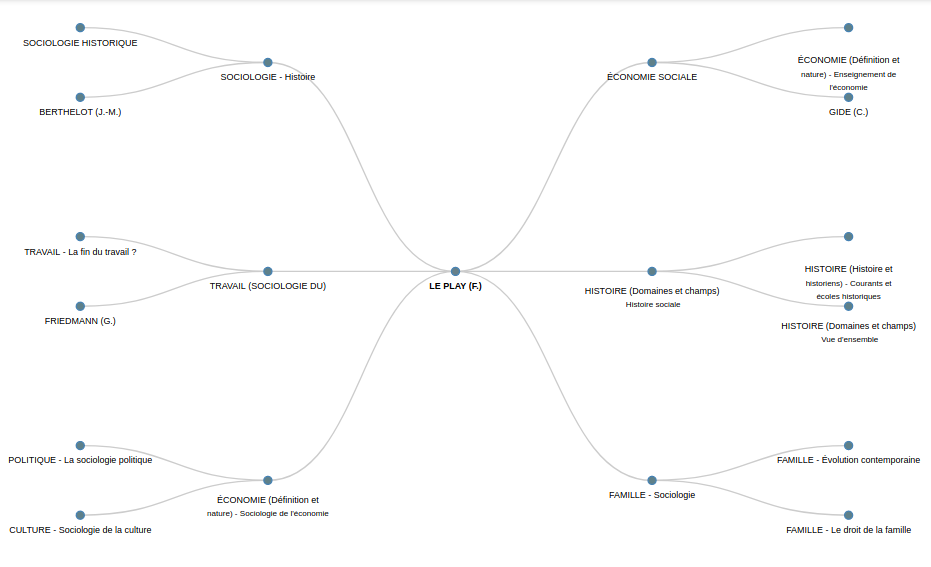
\includegraphics[width=16cm]{carte_mentaleLP}
    \label{carte_mentaleLP}
\end{figure}
Par ailleurs, Frédéric Le Play se trouve au croisement de nombreux champs intellectuels, à nous de voir comment nous pourrons le faire valoir dans notre projet. Il s'agit pour nous de relever un défi pour faire connaître un sociologue méconnu.



Lors de la présentation des sources dans le troisième chapitre, nous détaillerons l'importance des sources qui sont en notre possession ou en cours d'acquisition. 
Avant cela, il importe de présenter le deuxième projet sur lequel nous avons travaillé, au sein du Labex OBVIL.




\section{ELICOM}

A travers ELICOM, le Labex OBVIL 
\begin{quote}
\inquote {propose une recherche inédite sur la question de la valeur littéraire, envisagée au travers de l'étude de grands corpus numérisés qui prennent en compte, non seulement les textes eux-mêmes mais les circonstances et les modalités de leur publication et de leur réception\footnote{Laboratoire d'excellence OBVIL, \emph{Site web de l'enseignement supérieur et de la recherche}, URL : \url{https://cache.media.enseignementsup-recherche.gouv.fr/file/Fiches_Labex_2/63/8/OBVIL_207638.pdf} (visité le 04/09/2020).}}.
\end{quote}

Si les sources en elles-mêmes nous seront exposées plus en détail dans le chapitre suivant, présentons dès à présent les grands axes du projet\footnote{Cette présentation du projet est largement inspirée des documents qui ont été présentés afin d'obtenir les financements.}.

Retenu par l'appel à projet Émergence\footnote{Voir : Appel à projets Emergence , \emph{Site web de Sorbonne Universités}, \url{https://candidature.sorbonne-universites.fr/index.php?option=com_emundus&view=programme&id=111&Itemid=1521&lang=fr} (visité le 07/09/2020)} qui entend consolider l'excellence au c\oe ur des disciplines, accompagner les évolutions interdisciplinaires et ouvrir l'université sur la société, le projet ELICOM se révèle 
être ambitieux et innovant, car il est plus qu'une simple édition numérique de correspondance. 

\subsection{Pour une recherche collective et multidisciplinaire}

Tout d'abord, le présent projet semble s’inscrire dans un mouvement de recherche collective, national ou international. Mais cette inscription en fait bien apparaître la singularité : elle sort du cadre strictement littéraire pour s’ouvrir à des corpus de philosophie, de biologie, de mathématiques. Cette multidisciplinarité répond à la volonté de s’appuyer sur les collaborations institutionnelles, à l’intérieur de Sorbonne Université avec sa Bibliothèque riche en archives scientifiques, avec la Bibliothèque Nationale de France (BNF) dont Gallica offre d’immenses ressources de correspondances éditées en format image, voire en mode texte. Le labex OBVIL poursuit ainsi sa politique patrimoniale de recherche tout en accentuant sa réflexion sur les services qu’il peut offrir à la communauté dans laquelle il s’insère et à la communauté des chercheurs. 

\subsection{Un outil de réflexion et de recherche}

Cela signifie aussi que le caractère innovant du programme ne réside pas dans les correspondances elles-mêmes, même si le labex OBVIL apportera son savoir-faire et son expertise aux spécialistes d’un auteur qui éditent ou souhaitent éditer, au format numérique, une correspondance. Il réside avant tout dans la volonté forte de constituer autour d’un objet théorique – qu’est-ce que correspondre par lettres ?- une communauté de spécialistes venus de disciplines différentes pour penser les besoins éditoriaux en fonction des possibilités offertes par le numérique. La création d’une plateforme d’édition et de lecture répondra aux besoins multidisciplinaires tout en devenant un outil de réflexion et de recherche pour les communautés de chercheur.

L’ambition ultime sera de tester les résultats du présent programme sur des correspondances émanant non plus d’une élite savante, mais de communautés plus ordinaires, familiales, ou socio-professionnelles. Le projet ambitionne ce retour vers la vie ordinaire, sociale, professionnelle, citoyenne. 

\subsection{Trois modules}


Ces corpus, une fois édités - ce qui n’est qu’un préalable au projet pris en charge par le Labex OBVIL - forment un premier échantillon multidisciplinaire qui est exploité par les trois modules de la plateforme ELICOM : l’enrichissement, la fouille et l’exploitation.

\subsubsection{Enrichissement}

Ce premier module offre à chaque utilisateur la possibilité d’enrichir les textes édités à l’aide de balises TEI\footnote{Nous reviendrons sur tous ces termes dans la suite du mémoire.}, choisies à partir de ses propres questionnements, et en s’appuyant sur le manuel d’encodage pour correspondances mis au point par le consortium CAHIER\footnote{ Richard Walter (dir.), \emph{L’édition numérique de correspondances – guide méthodologique}, URL :  \url{https://cahier.hypotheses.org/guide-correspondance} (visité le 17/06/2020).}. Il lui permet également d’annoter chaque lettre en collaborant à la mise en place d’un apparat critique comme des notes savantes et des références bibliographiques, et de compléter les métadonnées.
Cet enrichissement participatif permet à terme d’adapter les corpus aux perspectives de recherche de chacun, et de mettre un ensemble de données et de métadonnées à disposition de la communauté scientifique.

\subsubsection{Fouille}

Ce second module ouvre ensuite à la fouille des textes et de leurs métadonnées, par un ensemble d’outils de \emph{text mining}. Il prévoit également un travail de modélisation sémantique, réalisé au cours du séminaire qui accompagne le développement de la plateforme, et qui s’appuie à la fois sur une construction systématique de ressources linguistiques à caractère polémique et sur des corpus de correspondances annotés manuellement par des experts. L’enjeu est de pouvoir exploiter ces données par des outils du Traitement automatique des langues (TAL) dans le but d’effectuer :
\begin{itemize}
    \item une analyse sémantique des controverses (identifier les postures et les positionnements de débats, de polémiques, etc.) 
    \item une analyse des enchaînements temporels (différenciant récit de vie et discours)
    \item une analyse thématique (autour des événements publics et privés)
    \item une analyse des rituels de la correspondance (formules de politesse, styles selon le destinataire) 
    \item un repérage des entités nommées\footnote{\inquote{On appelle entité nommée toute expression linguistique qui réfère à une entité unique du modèle de manière autonome dans le corpus.} Voir : Maud Ehrmann, \emph{Les Entitées Nommées, de la linguistique au TAL : Statut théorique et méthodes
de désambiguïsation}, Thèse de doctorat, Université Paris Diderot, 2008, URL : \url{https://hal.archives-ouvertes.fr/tel-01639190} (visité le 07/09/2020).}, etc.
\end{itemize}

L’ensemble de ces fonctionnalités doit permettre une exploration transversale des correspondances par le biais de requêtes croisées (par nature de la lettre, par thématique, par lieu, par âge ou sexe des correspondants, etc.), de manière à conduire l’utilisateur vers certains événements propres à la correspondance épistolaire.

\subsubsection{Exploitation}

Ce troisième module propose différents types de visualisation permettant une représentation et une analyse des données et des métadonnées des correspondances : des nuages de collocations, des réseaux (entités nommées et métadonnées), des cartographies par géolocalisation, des visualisations de relevés statistiques et des visualisations croisées par période et par fréquence de correspondances, par lieu et par auteur, etc.\\

Le projet étant très vaste, nous en sommes encore à la phase d'encodage en XML-TEI. C'est donc cette partie qui nous a été confiée lors de notre stage. Gérer un corpus aussi large est un véritable défi, notamment dans le choix des balises. C'est ce défi que nous avons dû relever. Mais avant cela, il faut penser l'édition. Ce sera l'objet de notre seconde partie. En attendant, il sera bon de considérer quelles sont les sources exploitées pour avoir meilleure vue d'ensemble du projet.




\chapter{Les sources des projets : des correspondances du XIX\up{e} siècle aux formes variées}

Les deux projets auxquels nous avons participé n'ont pas les mêmes caractéristiques tout en ayant de nombreux points communs, comme nous l'avons déjà souligné.

Pour le CRHXIX, l'objectif est de mettre à disposition une correspondance riche mais oubliée et peu connue et reconnue.
Pour OBVIL au contraire, l'objectif est de (re)mettre en valeur une correspondance qui a déjà été publiée, à laquelle on s’est déjà intéressée, qui est déjà en ligne, mais dont on voudrait faciliter l’exploitation, le croisement des sources, l'interopérabilité. 

Pour le projet d'édition numérique de la correspondance de Frédéric Le Play, nous travaillons sur un homme autour duquel se greffe tout un réseau. Pour ELICOM, c'est un réseau en soi que nous mettons en valeur.

Par ailleurs, pour le projet Le Play, c'est une approche plutôt classique d'édition. Pour ELICOM, c'est une démarche innovante.

Enfin, et c'est ce qui fait toute la différence des moyens employés, pour le projet Le Play, nous avons affaire à des manuscrits originaux numérisés ou à numériser, alors que pour ELICOM, nous travaillons sur des éditions imprimées qui ont été numérisées et sont disponibles sur Gallica.

Il est donc temps de présenter ces différents corpus du XIX\up{e} siècle.

\section{La mise en valeur de manuscrits}

Tout d'abord, le CRHXIX est en pleine phase d'acquisition de manuscrits de Frédéric Le Play sous une forme numérisée. .

La correspondance de Le Play est relativement dispersée. Elle se trouve principalement en Europe, plus particulièrement en France, mais certains manuscrits sont conservés en Suisse et en Italie par exemple. 

Il s'agit donc de contacter les différents lieux de conservation de ces manuscrits - bibliothèques,  archives privées et publiques etc. - demander leur numérisation en vue de leur transcription et encodage pour la future mise en ligne du manuscrit et de sa transcription.

Ce travail a été déjà bien entamé. 
Un premier inventaire provisoire, de plus de deux-mille lettres, a déjà été réalisé en 2005 par Stéphane Baciocchi et Antoine Savoye - spécialiste reconnu de Frédéric Le Play - paru dans la revue des \emph{Études sociales}\footnote{\cite{inventaire}}. Nous nous y sommes référée dans notre travail de prise en main du projet pour avoir une vue d'ensemble des sources. Nous nous y reportons donc également pour cette présentation des sources. 

\subsection{Trois fonds familiaux principaux}

Les archives de Frédéric Le Play ont été localisées dans trois fonds principaux : au château de Ligoure (Haute-Vienne), à la Bibliothèque de l'Institut de France (BIF) à Paris, ainsi qu'à la Société d'économie et de science sociales (SESS) à Paris.

\subsubsection{Château de Ligoure (Haute-Vienne)}
En 1856, Frédéric Le Play achète le domaine de Ligoure, y établissant une famille-souche\footnote{Principe selon lequel \inquote{l'un des fils demeure avec sa femme et ses enfants dans le foyer paternel en attendant la succession}, développé par Frédéric Le Play, expliqué ici par Emmanuel Todd, \inquote{Les familles dans l'Histoire}, \emph{Herodote.net}, URL : \url{https://www.herodote.net/Les_familles_dans_l_Histoire-article-1287.php} (visité le 08/09/2020).} à travers son fils, Albert Le Play. Frédéric Le Play y séjourne pendant l'été et retourne dans sa résidence parisienne durant l'hiver.

D'après l'inventaire réalisé par Antoine Savoye et Stéphane Baciocchi, on constate que
\begin{quote}
\inquote{de nombreuses lettres de Frédéric à son fils (1865-1881), notamment celles dans lesquelles il est question de la gestion du domaine agricole, y sont encore aujourd'hui conservées et propriété de l'arrière petite-fille d'Albert, Madame Thomas-Mouzon. Elles voisinent, dans les tiroirs et placards de la bibliothèque, avec celles que F. Le Play adressa à sa belle-fille, son « héritière-associée » (1867-1880), et quelques autres lettres des années 1866-1876. En attendant un inventaire plus précis de ce fonds, on peut d'ores et déjà penser que toutes les correspondances restées à Ligoure sont une partie de celles qui y ont été adressées après 1864\footnote{\cite{inventaire}}.}
\end{quote}

\subsubsection{Bibliothèque de l'Institut de France (Paris)}

Le fonds conservé à la BIF lui a été confié par Jean Albert Le Play, arrière petit-fils de Frédéric Le Play, en 1946. Il comporte un millier de lettres datées des années 1832-1882 et des liasses de notes manuscrites et de papiers divers.

Certaines sont adressées à Victor Legrand, directeur général des ponts et chaussées et des mines, au cours ou au retour de ses missions à travers l'Europe (1836-1846).
Il constitue le seul fonds public qu'il nous reste de Le Play et laisse à entendre que un bon nombre de papiers ont disparu. Le gros de la correspondance conservée est en lien, d'une part, avec les éditions successives et la diffusion de ses ouvrages la \emph{Réforme sociale en France}, l'\emph{Organisation du travail}, l'\emph{Organisation de la famille} et, d'autre part, avec la mise en place des UPS. Cet ensemble est daté des années 1860 et 1870. 

Comme le soulignent Antoine Savoye et Stéphane Baciocchi, 
\begin{quote}
    \inquote{le fonds public, ouvert depuis 1946 aux chercheurs, est celui où ont puisé tous les travaux de première main sur Le Play, sans toujours s'interroger explicitement sur les effets de sources, en l'espèce particulièrement discontinues et composites. On pourrait ici pointer l'inadéquation des récits biographiques linéaires fondés sur un tel matériau\footnote{\cite{inventaire}}.}
\end{quote}
D'où l'intérêt de notre travail qui permettra de mettre en ligne non seulement ce fonds déjà ouvert, mais aussi nombre de lettres encore inconnues du grand public et qui permettront de faire des recherches plus cohérentes sur Le Play et donneront l'occasion de voir apparaître de nouvelles études plus complètes.

\subsubsection{Société d'économie et de science sociales (Paris)}

Jean Albert Le Play conservait encore certaines lettres de son ascendant. Celles-ci ont été confiées en 1986 à la SESS. On y trouve plus de 200 lettres que Frédéric Le Play adressa à sa mère Rosalie Le Play-Auxilion (1833) et à sa femme Augustine Le Play-Fouache (1837-1877).\\

Ces trois fonds familiaux constituent 1167 lettres adressées à 49 correspondants.

\subsection{Des fonds dispersés à travers l'Europe}

A côté de ces trois massifs, la correspondance est particulièrement éclatée dans de nombreuses bibliothèques et centres d’archives, tant en France (Archives nationales, Bibliothèque nationale de France, bibliothèque Thiers, etc.) qu’à l’étranger (Angleterre, Belgique, Italie, Russie, etc.).

Les fonds complémentaires sont les ouvrages de Le Play, les enquêtes publiées, les revues du mouvement. Une large partie est disponible sur Gallica (\emph{La Réforme sociale en France}, 1864 ; \emph{Les Ouvriers européens}, 6 volumes entre 1877 et 1879 ; revue \emph{La Réforme sociale}, 1881-1934, etc.)\\
   
Enfin, on constate malheureusement que la correspondance autour de Le Play est lacunaire. Ainsi, aucune correspondance avec Albert de Saint-Léger et Adolphe Focillon, pourtant acteurs essentiels des premiers développement de la science sociale, n'a été retrouvée. Nous n'avons pas non plus trouvé trace d'Alexis Delaire, alors qu'il a eu un grand rôle à jouer dans l'organisation des UPS.

Par ailleurs, les correspondants étrangers sont rares, et aucune correspondance russe n'a été retrouvée, on pense surtout à Anatole de Demidoff, \inquote{commanditaire et employeur de Le Play durant une vingtaine d'années et qui lui a ouvert les portes de la Russie, découverte essentielle\footnote{\cite{inventaire}}.}


\subsection{Une correspondance au service de l'Histoire}

Le corpus, bien qu'incomplet, est largement prometteur. On y discerne déjà des thèmes principaux\footnote{Ces thèmes ont été relevés toujours par l'inventaire déjà nommé de 2006 que nous paraphrasons.}, qu'il est important d'avoir en mémoire pour les futurs choix éditoriaux :

\begin{itemize}
    \item La genèse des Ouvriers européens éclairée par la correspondance avec Jean-Baptiste Dumas et Augustin Cochin.
    \item L'organisation interne de la Société d'économie sociale (sur laquelle on ne possède pas d'archives pour le XIX\up{e} siècle) révélée par la correspondance avec Louis de Kergorlay.
    \item La volonté d'intervention publique de Le Play qui se manifeste à travers ses relations avec les catholiques libéraux (correspondance avec A. Cochin, Mgr Dupanloup et particulièrement Charles de Ribbe.
    \item La fondation expérimentale d'une « famille-souche » telle qu'elle apparaît dans la correspondance avec son fils, Albert.
    \item La conception du rôle de l'Église et la place de la religion dans la société (correspondance avec le père Hyacinthe). On y voit les importantes questions qu'y se posent autour du Concile Vatican I.
    \item La praxis réformatrice dont, lettres après lettres, Le Play précise sa conception à des interlocuteurs comme Emmanuel de Curzon et l'Écossais, David Urquhart.
\end{itemize}

Nous pouvons conclure, toujours avec Messieurs Antoine Savoye et Stéphane Baciocchi, que nous avons là \inquote{de quoi alimenter un vaste programme de travail, tant sur l'émergence des sciences sociales que sur les évolutions de la pensée sociale dans la France du Second Empire et de la III\up{e} République commençante\footnote{\cite{inventaire}}.}

\subsection{Nature des sources et première prise en main du projet}

L'ensemble de cette correspondance compte 2091 lettres échangées entre Frédéric Le Play et 94 correspondants entre 1837 et 1882.
Il s'agit donc de ne pas se perdre dans cette correspondance hétéroclite, à la fois active et passive.

Les premiers jours du stage ont donc été consacrés à un recensement des lettres qui nous ont été confiées\footnote{Le stage étant en télétravail, nous avons dû procéder à un versement par WeTransfer, service de transfert de fichiers en ligne.}.\begin{figure}[ht]
    \centering
    \caption{Fonds numérisés, extrait de l'inventaire}
    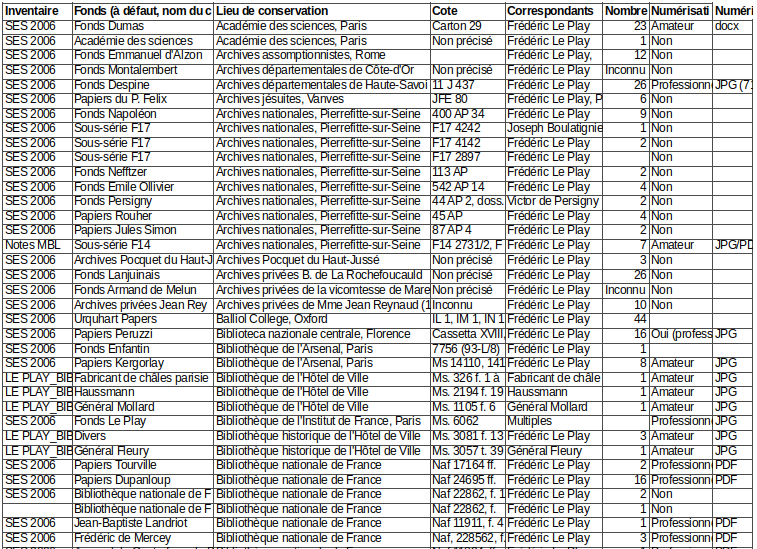
\includegraphics[width=16cm]{images/inventaire_numerisationsRHDL.png}
    \label{inventaire_numerisationsRHDL}
\end{figure} En effet, le seul document de référence pour comprendre les archives était l'inventaire de 2005. Nous ne disposons pas d’inventaire ou de description précise des fonds que nous avons pu récolter. Nous avons donc établi un tableau excel pour discerner quelles correspondances nous devions traiter en priorité, selon la qualité des numérisations que nous avions en notre possession. 
Nous nous sommes concentrée particulièrement sur les manuscrits écrits de la main de Frédéric Le Play afin de pouvoir commencer notre travail sur Transkribus, point que nous développerons davantage dans la deuxième partie.

Le CRHXIX est encore dans une phase d'acquisition des sources. Il en possède déjà des photocopies, matériau peu rentable pour notre future mise en ligne. Il détient également des numérisations, qui sont dans l'ensemble de qualité. Enfin, il possède des photos de médiocre qualité. Il sera nécessaire d'en demander par la suite les numérisations aux institutions en question.

Par la suite, nous avons eu accès à un fichier récapitulatif des transcriptions qui nous a été fort utile, et au cours de notre stage, un membre de l'équipe a également réalisé un fichier excel dont l'objectif était de faire un point sur la qualité des numérisations. Nous en trouvons ici\footnote{Fig. 3.1} un aperçu qui nous permet de voir l'ampleur des fonds.

La prise en main du projet est donc déterminée par la nature des sources en notre possession. Ceci vaut aussi bien pour le CRHXIX que pour le Labex OBVIL.





\section{De l'édition papier à l'édition numérique}

Pour ELICOM, les sources du projet sont bien différentes. En effet, bien que ce soient également des lettres du XIX{e} siècle, nous travaillons cette fois-ci non plus sur la source directement ou sur sa numérisation, mais sur des imprimés qui ont été numérisées. Pour cela, Gallica est une mine inépuisable ou presque.

\subsection{Gallica, une mine de savoirs}

Gallica est la bibliothèque numérique de la BNF. Elle regroupe plus de six millions de documents, livres au format Epub, journaux, revues, images, enregistrements sonores, cartes, manuscrits et vidéos. 

Parmi ces multiples documents, on trouve de nombreux ouvrages numérisés, dont d'anciennes éditions de correspondances du XIX\up{e} siècle. Ce sont elles qui ont été choisies dans le cadre du projet ELICOM pour être traitées afin d'être plus accessibles aux chercheurs et plus aisément fouillées. 

Pour notre projet, un cahier des charges avait déjà était dressé il y a deux ans, mettant en exergue les sources intéressantes repérées sur le catalogue de la BNF, et redirigeant vers les sources présentes sur Gallica. Plusieurs noms ressortent de cette analyse.

\subsubsection{Pierre-Joseph Proudhon}

Proudhon (1809-1865) reflète à lui seul la volonté de multi-disciplinarité d'ELICOM. Polémiste, journaliste, économiste, philosophe, politique et sociologue français, sa correspondance est riche de quatorze volumes\footnote{ \emph{Correspondance de P.-J. Proudhon}, \emph{BNF Catalogue général}, URL : \url{https://catalogue.bnf.fr/ark:/12148/cb35438908j} (visité le 08/09/2020).}. Précurseur de l'anarchisme, il est le seul théoricien révolutionnaire du XIX\up{e} siècle à être issu du milieu ouvrier.\\

Durant notre stage, nous avons pu réaliser l'extraction du premier volume, soit près de cent lettres. Les correspondants sont relativement nombreux. On y trouve notamment le journaliste et premier disciple de Fourier, Just Muiron (1787-1881),  le philologue Paul Ackermann (1812-1846) et l'orientaliste, sinologue et poète Guillaume Pauthier (1801-1873). Nous y reviendrons plus en détail dans la troisième partie de ce mémoire.

\subsubsection{Louis Pasteur}

Avec Louis Pasteur (1822-1895), dont nous avons retenu quatre volumes de correspondance\footnote{ \emph{Correspondance de Pasteur, 1840-1895}, \emph{BNF Catalogue général}, URL : \url{https://catalogue.bnf.fr/ark:/12148/cb32510650x} (visité le 08/09/2020).}, nous sommes face à un corpus plus scientifique, qui souligne encore une fois la volonté trans-disciplinaire d'ELICOM.

Néanmoins, nous devons préciser que nous n'avons pas eu à traiter ce correspondant durant notre stage.

\subsubsection{George Sand}

Nous n'avons pas non plus traité la correspondance de George Sand (1804-1876), riche de six volumes\footnote{\emph{Correspondance : 1812-1876 / George Sand, BNF Catalogue général}, URL :\url{https://catalogue.bnf.fr/ark:/12148/cb31293789z} (visité le 19/05/2020).}, correspondance cette fois d'une femme de lettres, depuis ses huit ans jusqu'à sa mort à l'âge de soixante-douze ans.

\subsubsection{Alphonse de Lamartine}

La correspondance de Lamartine (1790-1869), qui comporte six volumes\footnote{ \emph{ Correspondance de Lamartine, BNF Catalogue général}, URL : \url{https://catalogue.bnf.fr/ark:/12148/cb30725428p} (visité le 19/05/2020).}, est celle sur laquelle nous nous sommes le plus attardée, puisque c'est par elle que nous avons commencé notre stage et que nous nous sommes familiarisée avec les procédures à suivre.

Nous nous sommes attelée à l'extraction du premier volume, comportant près de cent lettres, où Lamartine correspond avec ses meilleurs amis, Prosper Guichard de Bienassis et Aymon de Virieu.
Le deuxième volume comporte un nombre plus important de correspondants, parmi lesquels figurent encore Aymon de Virieu, et aussi Laurent de Jussieu, Fortuné de Vaugelas, Éléonore de Canonge, la marquise de Raigecourt, le baron de Vignet, le comte de Saint-Mauris, le duc de Rohan, l'abbé Dumont et Eugène de Genoude.    

\subsubsection{Félicité de Lamennais}

L'Abbé Félicité de Lamennais (1782-1854) présente une correspondance active forte de deux volumes\footnote{\emph{ Correspondance de Lamennais, BNF Catalogue général}, URL : \url{https://catalogue.bnf.fr/ark:/12148/cb30728369q} (visité le 08/09/2020).}, adressée pour ce qui est du premier volume que nous avons traité, pour la plupart à des personnes de son rang, telles que Mademoiselle Cornulier de Lucinière, Monsieur le Comte de Senfft et Madame la Comtesse de Senfft, ou encore au Marquis de Coriolis\footnote{Les correspondants sont nommés avec leurs titres dans cette correspondance.}. Un volume représente en réalité trois tomes, et donc près de deux-cent lettres d'une longueur assez importante en général. Le premier volume regroupe la correspondance de 1818 à 1823. Le deuxième couvre les années 1826-1827. Le troisième est entièrement consacré à l’année 1828.

\subsection{Un traitement adapté à la nature des sources}

Comme nous l'avons souligné plus haut, la nature des sources détermine en quelque sorte leur traitement ; même si nous avons encore une certaine liberté dans le choix des outils, ceux-ci doivent cependant s'adapter aux caractéristiques du corpus.

Ici, nous avons affaire à un corpus assez vaste et hétérogène. Les choix d'éditeurs se sont avérés être différents. Pour chaque correspondant, le cahier des charges met en avant un degré de difficulté selon les marqueurs présents ou non et permettant d'extraire les lettres avec plus ou moins de difficultés. La qualité de l'océrisation joue également un rôle et demande une relecture plus ou moins précise. Nous y reviendront plus spécifiquement dans les troisième et quatrième parties de notre mémoire.\\

En attendant, il convient de souligner qu'avant d'extraire des données et surtout de les traiter, il faut avoir une idée assez précise de ce que l'on veut en faire. 
En effet, il s'agit là, que ce soit pour ELICOM ou l'édition numérique de la correspondance de Frédéric Le Play, d'une édition numérique.

C'est d'une part une \emph{édition} : une édition ne se fait pas à la légère. Elle s'accompagne de choix éditoriaux sentis et pesés.

C'est une édition \emph{numérique} : le numérique apporte son enrichissement mais aussi ses contraintes. Une édition numérique ne se pense pas de la même façon qu'une édition papier. 

C'est une édition numérique de \emph{correspondance} : elle doit donc prendre en compte les caractéristiques du genre épistolaire, notamment avec les rituels épistolaires.

Il est donc opportun de s'arrêter à toutes ces questions. Ce sera l'objet de notre deuxième partie.

\part{Penser l'édition numérique de correspondance}




\chapter{Bilan scientifique}


\section{Réflexions autour de l’édition numérique de correspondance. Une communauté scientifique grandissante}

\subsection{Des communautés de réflexion, des projets et des publications...}


Nombreux sont les communautés, réseaux, groupes de travail qui se retrouvent autour de réflexions sur l'édition numérique de correspondance. Celle-ci a en effet le vent en poupe depuis quelques années. Des sites se créent chaque année, nous en donnerons quelques exemples par la suite\footnote{Voir 4.2}. 

En attendant, il est intéressant pour nous de voir quelles sont les personnes ou communautés qui \oe uvrent autour de l'édition numérique de correspondance. 

\subsubsection{\emph{TEI: Correspondence SIG}}

Le \emph{Special Interest Group} (SIG) ou pôle d'intérêt commun TEI sur la correspondance, sous la direction de Monsieur Stefan Dumont, de l'Académie des sciences de Berlin-Brandebourg, et de Madame Sabine Seifert, de l'Université de Potsdam, cherche à rassembler des universitaires intéressés par la création d'éditions scientifiques numériques de correspondance. Son but est donc de développer un ensemble de balises propres à différentes formes de correspondance en XML-TEI, ainsi que de créer des tutoriels et des modèles de bonnes pratiques\footnote{\emph{TEI : Correspondence SIG, Site web de la TEI}, URL : \url{https://tei-c.org/Activities/SIG/Correspondence/} (visité le 09/09/2020).}.

Par ailleurs, le \emph{Correspondence SIG} tient une page Wiki intitulée \emph{SIG:Correspondence} et mise à jour régulièrement\footnote{Voir \emph{SIG:Correspondence, Page Wiki}, URL : \url{https://wiki.tei-c.org/index.php/SIG:Correspondence} (visité le 09/09/2020).}, et il envoie ses réflexions à une liste de diffusion, ouverte à tous ceux qui désirent s'y inscrire.\\

Depuis 2008, le SIG organise des journées annuelles autour de la correspondance. Celle de 2013 qui s'est tenue à Rome\footnote{Voir le compte-rendu, \emph{Site web de la TEI}, \url{https://tei-c.org/activities/sig/correspondence/tei-sig-on-correspondence-minutes-rome-oct-3-2013/} (visité le 09/09/2020).} a été particulièrement fructueuse, puisqu'elle a vu la création d'un groupe de travail intitulé \inquote{correspDesc} et composé de Madame Sabine Seifert, Messieurs Marcel Illetschko et Peter Stadler, dont l'objectif a été de créer et faire approuver un nouvel élément XML-TEI nommé \citecode{<correspDesc>}, décrivant l'action de la correspondance, notamment l'expéditeur et le destinataire\footnote{\emph{correspDesc, Site web de la TEI}, URL : \url{https://tei-c.org/release/doc/tei-p5-doc/fr/html/ref-correspDesc.html} (visité le 09/09/2020).}. Celui-ci est une référence aujourd'hui dans l'édition numérique de correspondance et nous a été précieux pour notre travail.\\

Afin de mieux appuyer leurs réflexions autour de l'édition numérique de correspondance, des publications sortent pour soutenir les chercheurs et ingénieurs de recherche dans leurs travaux d'édition. Ainsi, Stefan Dumont, Susanne Haaf et Sabine Seifert ont publié en 2018 un manuel intitulé \emph{Encoding Correspondence. A Manual for Encoding Letters and Postcards in TEI-XML and DTABf}\footnote{\emph{Encoding Correspondence. A Manual for Encoding Letters and Postcards in TEI-XML and DTABf, Site web Encoding Correspondence}, URL : \url{https://encoding-correspondence.bbaw.de/v1/} (visité le 05/05/2020).}. Le SIG est donc riche en initiatives pour guider ceux qui veulent se lancer dans l'édition numérique de correspondance. Il continue à 
être régulièrement alimenté et complété au fil des améliorations et découvertes techniques. \\

\subsubsection{Autres initiatives techniques du \emph{Correspondence SIG} : le format CMIF et le service <CorrespSearch>}

Le format\footnote{Un format de données est la façon dont est représenté (codé) un type de données, sous forme d'une suite de bits. Voir \inquote{Format de données}, \emph{Wikipédia}, URL : \url{https://fr.wikipedia.org/wiki/Format_de_donnees} (visité le 10/09/2020).} CMIF (\emph{Correspondence Metadata Interchange Format}) est basé sur le module <correspDesc>. Son objectif est de pouvoir fournir les métadonnées les plus importantes permettant de partager des corpus de lettres quel que soit leur format\footnote{Tout ce passage s'appuie largement sur \emph{L’Édition numérique de correspondance ; Guide méthodologique, Site web du consortium CAHIER}, URL : \url{https://cahier.hypotheses.org/files/2018/03/Correspondance_CAHIER.pdf} (visité le 17/06/2020).}. 
Ce format CMIF permet de créer des fichiers XML rassemblant des éléments \citecode{<correspDesc>}, chacun représentant une lettre éditée. Chaque élément \citecode{<correspDesc>}, utilisé de manière très restrictive, se borne aux informations suivantes:
\begin{itemize}
    \item Nom de l’expéditeur et ID contrôlée par l’autorité
    \item Nom du destinataire et ID contrôlée par l’autorité
    \item Date d’écriture et de réception
    \item Lieu d’écriture et de réception (nom et ID contrôlée par l’autorité)
    \item Numéro de la lettre dans l’édition savante
    \item URL de la lettre éditée
\end{itemize}
Les identifiants ou ID proviennent des fichiers d’autorité pour les personnes et les lieux, \emph{GeoNames}\footnote{\emph{The GeoNames geographical database}, URL : \url{https://www.geonames.org/} (visité le 10/09/2020).} pour les lieux, VIAF (\emph{Virtual International Authority File}) ou \emph{data.bnf}\footnote{\emph{Des fiches de référence sur les auteurs, les œuvres et les thèmes, data.bnf}, URL : \url{https://data.bnf.fr/} (visité le 10/09/2020).} pour les identités\footnote{Pour plus d'informations sur le CMIF, voir : \emph{
Perspectives of the further development of the Correspondence Metadata Interchange Format (CMIF), Site web digiversity, URL : \url{https://digiversity.net/2015/perspectives-of-the-further-development-of-the-correspondence-metadata-interchange-format-cmif/} (visité le 09/09/2020).}}.\\

\begin{figure}[ht]
    \centering
    \caption{Fonctionnement du \emph{correspSearch - Site web du correspSearch} en 2020}
    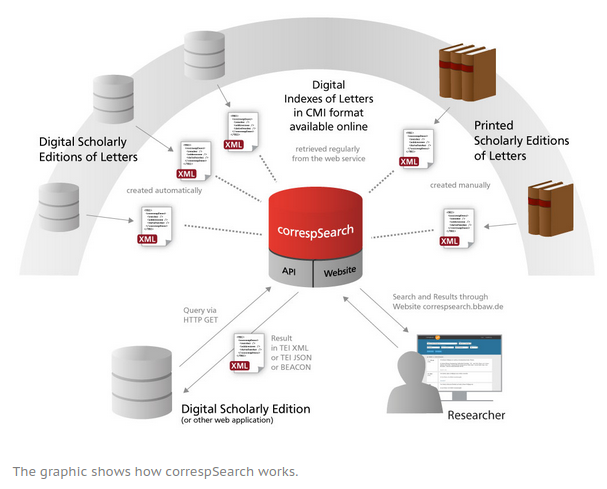
\includegraphics[width=16cm]{images/correspSearch.png}
    \label{correspSearch}
\end{figure}

Le service <CorrespSearch> est une interface de programmation applicative (API, \emph{Application Programming Interface}) destinée à être encapsulée dans une page Web, permettant de retrouver un ensemble de métadonnées identifiant des projets de correspondance (il ne s’agit pas d’un moteur de recherche avec une interface complète). Pour cela il faut qu’un projet d’édition de correspondance expose ses métadonnées afin de les rendre publiques à d’autres projets. Cet échange de données est basé sur la transmission de fichiers XML au format CMIF. Le schéma ci-dessous\footnote{Fig. 4.1} permet de mieux en comprendre le fonctionnement.
Une page web a par ailleurs été créée autour du CorrespSearch\footnote{\emph{About our web service. The idea behind correspSearch, Site web du CorrespSearch}, URL : \url{https://correspsearch.net/index.xql?id=about&l=en} (visité le 09/09/2020). La présente explication s'appuie largement sur cet article.}\\

Nous reviendrons en quatrième partie sur l'importance de ces pratiques, standards, formats et leur mise en pratique dans nos projets.



\subsubsection{Le consortium CAHIER}

Parmi les groupes de travail se retrouvant autour de l’édition numérique de correspondance, nommons particulièrement le consortium CAHIER (Corpus d’Auteurs pour les Humanités, Informatisation, Édition, Recherche). Celui-ci, constitué en fédération en 2011 dans le cadre de l’infrastructure \inquote{CORPUS} (désormais intégrée à la TGIR (Très grandes infrastructures de recherche) Huma-Num), CAHIER est un consortium interdisciplinaire de projets numériques, en accès libre, menés principalement dans les domaines des «corpus d’auteurs», qu’ils relèvent de la littérature, de la philosophie ou d’une thématique liée à une école ou à une pratique.

Comme elle le souligne elle-même\footnote{Accueil, \emph{Consortium CAHIER}, URL : \url{https://cahier.hypotheses.org/le-consortium} (visité le 17/06/2020).}, la
    \inquote{fédération des différents projets existants ou projetés en France leur donne l’opportunité et les ressources} entre autres pour :
\begin{itemize}
    \item augmenter l’acquisition de données de qualité (image et texte) tout en tenant compte des limites de taille
    \item proposer des normes de transcription suivant des objectifs éditoriaux clairement énoncés
    \item permettre leur indexation
    \item tester les différents modèles d’affichage du mode texte et du mode image et opérer des choix pertinents en fonction des publics
    \item offrir des métadonnées compatibles avec les standards de catalogage et d’archivage, d’identification et de protection des données ; moissonnage par Europeana, Isidore, Gallica [...]
    \item  offrir les moyens d’évoluer vers le web sémantique, la visualisation, les entrepôts de données, les modes de représentation d’ensembles documentaires, et vers l’annotation collaborative.
    \end{itemize}


Le consortium CAHIER, répondant aux objectifs qu'il s'est fixé, a publié en 2018, grâce au groupe de travail EVENT (Evaluation et Valorisation des Editions Numériques de Textes) un ouvrage intitulé \emph{Les publications numériques de corpus d’auteurs – Guide de travail, grille d’analyse et recommandations}\footnote{\emph{Les publications numériques de corpus d’auteurs, Site web du consortium CAHIER}, URL : \url{https://cahier.hypotheses.org/guides-juridiques/les-publications-numeriques-de-corpus-dauteurs} (visité le 09/09/2020).}. La même année, le groupe de travail \inquote{Correspondance} a publié un guide méthodologique rassemblant des recommandations pour l’édition numérique de correspondance, intitulé \emph{L’Édition numérique de correspondance ; Guide méthodologique}\footnote{\emph{L’Édition numérique de correspondance ; Guide méthodologique, Site web du consortium CAHIER}, URL : \url{https://cahier.hypotheses.org/files/2018/03/Correspondance_CAHIER.pdf} (visité le 17/06/2020).} et qui nous a été très précieux pour nos deux projets.\\

Par ailleurs, depuis plusieurs années, la correspondance épistolaire conduit à de nombreuses réflexions philologiques menées par d'autres groupes de recherche comme l'AIRE (Association Interdisciplinaire de Recherches sur l'Épistolaire)\footnote{Voir \emph{Association Interdisciplinaire de Recherches sur l'Epistolaire}, URL : \url{http://www.epistolaire.org/} (visité le 1/09/2020).}, fondée en 1981, mais à portée plus générale. Toutefois, elle est consciente que l'\inquote{édition électronique
paraît particulièrement adaptée à ce texte discontinu, toujours inachevé et se prêtant davantage à la recherche qu’à la lecture suivie}\footnote{Colloque international « Éditer les correspondances », \emph{Site web de l'AIRE}, URL : \url{http://www.epistolaire.org/evenements/editer-les-correspondances/} (visité le 10/09/2020} et a organisé dans ce sens, avec le Centre d’Étude et de Recherche Éditer/Interpréter de l’Université de Rouen (CÉRÉDI), un colloque dès 2007.

Nombreuses sont donc les recherches dans ce sens.

\subsection{...au service de normes et standards adaptés à la correspondance}

Comme nous l'avons vu, tous ces groupes de travail font avancer la réflexion sur l'édition numérique de correspondance, et ceci avec des normes et standards propres. Revenons sur leur définition.

\subsubsection{Normes et standards...}

En anglais, un seul terme est employé, celui de \emph{standard}. En français, on use d'une distinction. 

Un \textbf{standard} est un ensemble de recommandations développées et préconisées par un groupe représentatif d’utilisateurs\footnote{Voir \emph{Indexation de ressources, Site web du ministère de l'éducation nationale éduscol}, URL : \url{https://eduscol.education.fr/numerique/dossier/archives/metadata/normes-et-standards} (visité le 10/09/2020) ou encore : \url{https://slideplayer.fr/slide/13821861/} (visité le 10/09/2020).}. C'est donc un format élaboré par un petit nombre d’acteurs et adopté par des consortiums, des forums, c'est-à-dire des organisations non officielles.

En revanche, une \textbf{norme} est un document de référence élaboré par un organe de normalisation reconnu comme l’Organisation internationale de normalisation (ISO \emph{International Organization for Standardization}) et l’AFNOR (Association française de normalisation) en France.

Ainsi, le W3C (\emph{World Wide Web Consortium}) a en charge la normalisation de l'ensemble des protocoles d'Internet avec les standards de base comme HTTP, HTML et XML, ou encore des standards autour de l'interopérabilité et des services Web comme SOAP, des standards concernant les documents et le multimédia comme HTML, XML, CSS, et des standards liés à la sémantique et à la description de ressources come XML Schema et RDF pour n'en nommer que quelques-uns\footnote{\emph{Idem.}}.

\subsubsection{...pour l'édition numérique de correspondance}

En parlant des communautés scientifiques, consortiums et groupes de travail qui les pensent, nous avons donc déjà évoqué certains de ces standards ou normes fort utiles pour les éditions numériques de correspondance en général et donc pour nos projets en particulier.

Ainsi, le DC (\emph{Dublin Core}) est un standard de métadonnées consensuel établi par des professionnels provenant de diverses disciplines telles que la bibliothéconomie, l'informatique et le balisage de textes.

\subsubsection{XML}

Avec l'encodage des textes, nous sommes particulièrement concernés par XML (\emph{Extensible Markup Language}) qui provient de l'ancien standard SGML (\emph{Standard Generalized Markup Language}). XML est \inquote{un format de données pur, très simple et documenté, conçu pour la description des documents textuels}\footnote{Voir Ariane Pinche, \inquote{Séance 1}, \emph{Cours M2 TNAH XML}, URL : \url{https://github.com/ArianePinche/coursTNAH_XML-TEI/blob/master/seance01/InitiationXML.md} (visité le 09/10/2020).}, ne possédant pas de jeu de balises prédéfini, et respectant les recommandations du W3C. 

Il a l'avantage de faciliter d'une part la lisibilité par les machines et par l’œil humain, d'autre part l’échange de données, et enfin la migration vers d’autres plates‐formes, d’autres logiciels, et formats.

Nous reviendrons dans la quatrième partie sur l'intérêt d'avoir un document structuré, et sur la structure générale du document XML. Ce qui nous intéresse ici est surtout d'avoir une vue d'ensemble des efforts de réflexions faits jusqu'à ce jour autour de l'édition numérique de correspondance et de voir quels normes et standards on utilise dans ce domaine.

\subsubsection{TEI}

Or, la TEI s'avère être particulièrement intéressante pour nos projets. 
Les avantages du XML TEI sont de s’intéresser au sens du texte plutôt qu’à son apparence, d'être indépendant de tout environnement logiciel particulier, et d'avoir été conçu par la communauté scientifique, qui est aussi en charge de son développement continu.
Nous avons déjà parlé du TEI consortium plus haut.
Voyons ce qu'est véritablement la TEI.

TEI est \inquote{un set de balises prédéfini et documenté dans les TEIguidelines\footnote{Voir \emph{TEIguidelines, Site web de la TEI}, URL : \url{https://tei-c.org/guidelines/} (visité le 10/09/2019)} qui permet de procéder à une description ``scientifique'' et ``sémantique'' d’un texte}\footnote{Ariane Pinche, \inquote{Séance 3}, \emph{Cours M2 TNAH XML}, URL : \url{https://github.com/ArianePinche/coursTNAH_XML-TEI/blob/master/seance03/TEI.md} (visité le 10/09/2020).}.  Il s'agit d'un format de codage de documents dit « structuré » : il a besoin d'un langage, XML, pour aider à la saisie d'un texte en lui donnant une structure compatible à la fois avec les exigences des différentes communautés qui l'utilisent et avec les possibilités des outils de consultation\footnote{Définition donnée dans le \emph {Manuel d'encodage TEI
Renaissance et temps modernes}, URL : \url{http://www.bvh.univ-tours.fr/XML-TEI/ManuelWeb/Manuel_TEI_BVH.html} (visité le 11/09/2020).}. 

TEI (All) n’est pas un schéma à proprement parler, mais plutôt un \emph{framework}\footnote{Un framework est un ensemble cohérent de composants logiciels structurels, qui sert à créer les fondations ainsi que les grandes lignes de tout ou d’une partie d'un logiciel (architecture). Voir à ce sujet \inquote{\emph{Framework}}, \emph{Wikipedia}, URL : \url{https://fr.wikipedia.org/wiki/Framework} (visité le 10/09/2020).}, utile à la conception de son propre schéma. Il est
fortement déconseillé d’utiliser un schéma englobant l’intégralité de la
TEI. La conception d’un modèle adapté à ses données et son projet
est extrêmement importante, et c'est ce qui va nous intéresser par la suite : comment construire un schéma propre à la correspondance en général (ce sur quoi les communautés scientifiques se penchent) et ceci fait, comment l'adapter à chacun de nos projets en particulier ?

Par ailleurs, d'autres langages s'avèrent être utiles pour générer des fichiers XML, comme le langage de programmation \emph{Python} dont nous nous sommes servie dans le projet ELICOM, nous y reviendrons.

\subsection{Des outils au service de l'édition numérique}

Lors de nos stages, nous nous sommes appuyée sur nombre d'outils pour mener à bien nos projets.

Plusieurs d'entre eux étaient en libre accès. Parmi les éditeurs de texte, retenons particulièrement \emph{Sublime Text}. \emph{Oxygen XML Editor} nous a rendu aussi d'immenses services, notamment par son exigence et sa rigueur, veillant à la bonne indentation et la \emph{TEI conformance} de nos fichiers XML. Elle est distribuée pour tous les systèmes d’exploitation. Elle est sous licence propriétaire.

Pour la formation des expressions régulières ou REGEX (\emph{regular expression}), nous avons eu recours à un service en ligne \emph{regular expressions 101}\footnote{\emph{regularexpressions101}, URL : \url{https://regex101.com/} (visité le 10/02/2020).}. Quant à la transcription, nous avons eu recours à Transkribus, nous y reviendrons également. 

En bref, le choix est vaste, les outils nombreux.\\

Passons du théorique à la pratique et penchons-nous désormais sur les premières réalisations d'édition numérique de correspondance. En effet, il ne s'agit pas pour nous de tout inventer à partir de rien, mais au contraire de nous inspirer de travaux de référence déjà réalisés.

\section{Avec de nombreuses réalisations}

Les éditions numériques de correspondances, en cours ou déjà achevées, sont nombreuses. Dressons-en une liste non-exhaustive. On peut citer notamment\footnote{Voir Annexes A.1} :
\begin{itemize}
    \item L'édition numérique de la correspondance de D'Alembert sous la houlette de l'Institut de France, avec plus de deux-mille lettres\footnote{Voir \emph{Accueil}, D'Alembert en toutes lettres, URL : \url{http://dalembert.academie-sciences.fr/Correspondance/} (visité le 10/09/2020).}.
    \item La plateforme EMAN (Édition de Manuscrits et d'Archives Numériques\footnote{\emph{Accueil}, EMAN, URL : \url{http://eman-archives.org/EMAN/} (visité le 11/09/2020).})
diffuse des corpus en respectant les standards de l'édition numérique et de l'interopérabilité. Ainsi, elle abrite le projet CORREZ (Édition des lettres internationales adressées à Émile Zola) de 
    l'Institut des textes et manuscrits modernes (ITEM) - unité mixte de recherche entre l'ENS (École Normale Supérieure) et le CNRS (Centre national de la recherche scientifique). Plus de deux-mille quatre-cent lettres sont déjà en ligne\footnote{\emph{CORREZ - Édition des lettres internationales adressées à Émile Zola}, EMAN, URL : \url{http://eman-archives.org/CorrespondanceZola/} (visité le 11/09/2020)}.
   \item Plus de onze-mille lettres de Juliette Drouet à Victor Hugo sont déjà en ligne dans un site dédié\footnote{\emph{Accueil}, Juliette Drouet, Lettres à Victor Hugo, URL : \url{http://www.juliettedrouet.org} (visité le 02/07/2020)}.
    \item La correspondance inédite du géomètre Gaspard Monge (1746-1818) est déjà disponible en ligne\footnote{Voir \emph{La correspondance inédite du géomètre Gaspard Monge (1746-1818)}, EMAN, URL~: \url{http://eman-archives.org/monge/} (visité le 10/09/2020)}.
    \item Le Labex Obvil a déjà édité la correspondance de Jean Paulhan, disponible son site\footnote{Voir \emph{Correspondance de Jean Paulhau}, Site web OBVIL, URL : \url{http://obvil.sorbonne-universite.site/corpus/paulhan/} (visité le 10/09/2020)}.
    \item HUMA-NUM a édité la correspondance de l'éditeur et libraire Marc-Michel Rey\footnote{\emph{Marc Michel Rey}, HUMA-NUM, URL : \url{http://rey.huma-num.fr/presentation} (visité le 10/09/2020)}.
\end{itemize}

On pourrait allonger la liste d'une quarantaine de noms d'édition numériques de correspondance, mais ce n'est pas notre propos. Quoi qu'il en soit, il est intéressant ici de voir combien ces éditions sont de plus en plus nombreuses et présentes sur le \emph{cloud}.

    \begin{figure}[ht]
    \centering
    \caption{Lettre d'Adolf von Buch à Louis de Beausobre (Magdebourg, 15 janvier 1761), \emph{Lettres et textes : Le Berlin intellectuel des années 1800}}
    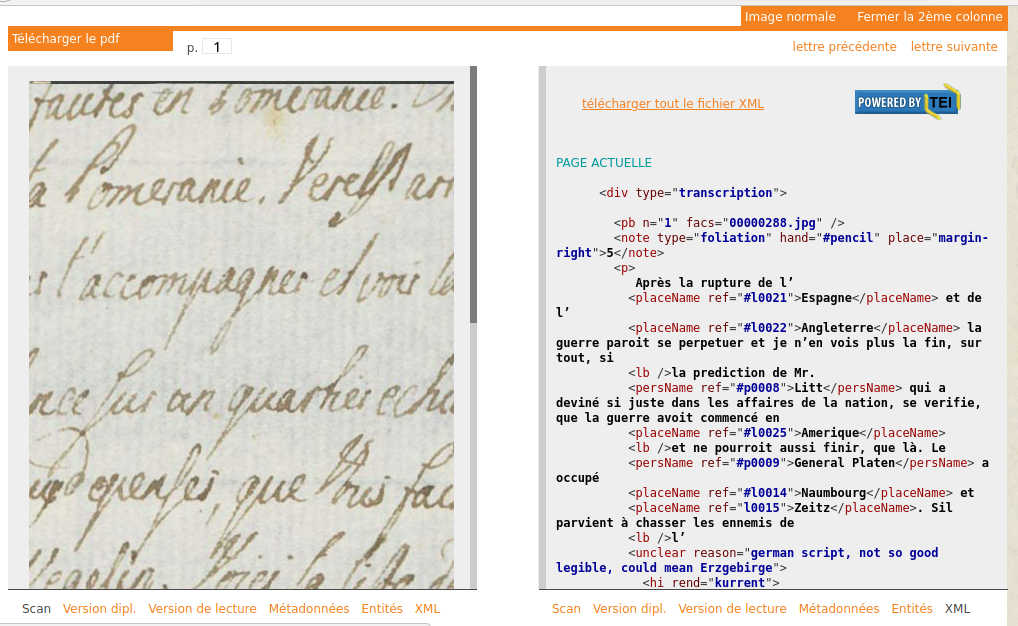
\includegraphics[width=16cm]{images/berlin_lettre.png}
    \label{berlin_lettre}
\end{figure}

Pour nous, trois éditions numériques nous ont particulièrement inspirées, pour l'architecture du site et les choix d'encodage, à savoir :
\begin{itemize}
    \item L'édition électronique des lettres de Flaubert, dirigée par Yvan Leclerc et Danielle Girard, avec la collaboration d'une trentaine de chercheurs et mise en ligne en 2017. Celle-ci présente les manuscrits et leurs transcriptions, ce qui est également notre intention, et leur site comporte une organisation intéressante que nous aimerions partiellement reproduire\footnote{\emph{Correspondance}, Site web du Centre Flaubert, URL : \url{https://flaubert.univ-rouen.fr/correspondance/edition/} (visité le 17/06/2020)}. 
    \item L'édition numérique de la correspondance de Proust. \inquote{L’édition des lettres de Proust a été l’objet, depuis plus de huit décennies, de recherches intenses qui convergent aujourd’hui dans le projet Corr-Proust, mené dans le cadre de la collaboration franco-américaine du Consortium ``Proust21''} : ainsi le projet est-il présenté sur leur site \emph{Corr-Proust}\footnote{\emph{Le Projet, Corr-Proust}, URL : \url{http://proust.elan-numerique.fr/presentation/project} (visité le 08/06/202).}.

    \item L'édition numérique des correspondances berlinoises au XIX\up{e} siècle, intitulée \emph{Lettres et textes : Le Berlin intellectuel des années 1800}\footnote{\emph{Lettres et textes : Le Berlin intellectuel des années 1800}, URL : \url{https://www.berliner-intellektuelle.eu/?fr} (visité le 19/05/202).} nous a particulièrement inspirée pour l'encodage, d'autant plus qu'elle a été réalisée par des spécialistes tels que Madame Sabine Seifert. Ci-dessus se trouve une capture d'écran du site avec d'un côté le manuscrit, de l'autre l'encodage en XML-TEI\footnote{Le manuscrit a été volontairement zoomé pour la capture d'écran.}.
\end{itemize}

Ainsi, nombreuses sont déjà les éditions numériques de correspondance. \\

Après avoir donc vu quelles communautés scientifiques guidaient les choix et les standards autour de l'édition numérique de correspondance, ainsi que les premières réalisations d'éditions, penchons-nous sur les problématiques et spécificités qu'elles supposent.



\chapter{Problématiques et spécificités de l'édition numérique de correspondance}

L'édition numérique de correspondance questionne. Nous l'avons vu à travers tous les groupes de recherche qui travaillent dessus.
Considérons plus spécifiquement les problématiques et spécificités qu'elle entraîne : c'est une édition, et numérique, et de correspondance, des termes à prendre en compte et qui sont tous à peser.

\section{Édition et numérique}

\subsection{Trois niveaux d’édition}

Tout d'abord, une édition est quelque chose de pensé. On entend par édition (papier ou numérique) le fait de reproduire et diffuser une \oe uvre, ici intellectuelle. 

Or, le numérique est par excellence un moyen de diffusion, et il permet un accès plus large au savoir.

On distingue trois types ou niveaux d'édition dans le numérique, d'après le guide de travail intitulé \emph{Les publications numériques de corpus d’auteurs}\footnote{Ioana Galleron, Marie-Luce Demonet, Cécile Meynard, Idmhand Fatiha, Elena Pierazzo, et al., \emph{Les publications numériques de corpus d’auteurs - Guide de travail, grille d’analyse et recommandations}, 2018, URL : \url{https://halshs.archives-ouvertes.fr/halshs-01932519/document} (visité le 05/05/202).} : 

Tout d'abord, il y a les \inquote{archives éditorialisées} qui proposent des collections d'images et, ou de textes, pour permettre la consultation de ressources rares et ce de façon rapide, avec une correction minimale des fautes d'océrisation. C'est le niveau d'édition le moins élaboré. Nous sommes allée plus loin pour nos deux projets.

Le deuxième type ou niveau de publication est l'édition de lecture ou \inquote{\emph{reading edition}}. Le texte a été bien relu et il est documenté de choix éditoriaux et autres accompagnements. Nos projets se rapprochent davantage de ce type d'édition ainsi que du troisième qu'est l'édition enrichie.

Ce dernier type d'édition est le plus poussé. Le texte est très enrichi, avec de nombreuses informations documentaires et contextuelles.

Il est à noter que les frontières entre chacune de ces trois types d'édition restent un peu floues. Pour nos projets, nous nous situons donc entre les deuxième et troisième types d'édition.

\subsection{Cinq dimensions à prendre en compte}

Par ailleurs, les éditions numériques ont cinq dimensions fondamentales. Elles ont certains points communs avec l'édition papier, et d'autres plus spécifiques\footnote{Voir en annexe (A.2) à ce sujet la grille d'évaluation des publications numériques de corpus d'auteur, tirée du guide déjà cité (note 1). }.

\subsubsection{Le texte}
Tout d'abord, tout comme l'édition papier, l'édition numérique dispose d'un texte : pour nos deux projets, ce sont des correspondances du XIX\up{e} siècle. 
La publication de ces textes doit respecter certaines règles, à savoir que le texte publié doit être complet, et les choix éditoriaux explicités et appliqués de façon stable sur l'ensemble du texte. Il peut être aussi intéressant de comparer la nouvelle version publiée avec les précédentes. \\

Tout d'abord, l'édition des textes nécessite une numérisation soigneuse et de qualité. Pour ELICOM, nous ne sommes pas concerné par cela, mais pour l'édition numérique de la correspondance de Frédéric Le Play, nous sommes encore en cours de numérisation\footnote{Nous reviendrons sur cette question de la numérisation lors de la partie III sur l'acquisition des données.}. En effet, \inquote{la lisibilité des images est essentielle}, et il est nécessaire d'avoir une bonne résolution de DPI (\emph{Digit per Inch} ou point par pouce) ainsi qu'une \inquote{juste évaluation des besoins de stockage et d'infrastructure matérielle pour la diffusion/communication de celles-ci}\footnote{\emph{Idem.} p. 7.}. Pour aucun des deux projets, nous ne nous sommes penchée sur la question du stockage. Cela reste un point à éclaircir particulièrement pour le projet du CRHXIX. 

Enfin, la publication en mode texte nécessite d'expliciter les choix scientifiques de normalisation et modernisation. 
Pour ELICOM, normalisation et modernisation sont notre politique, sachant que les chercheurs n'auront pas accès au manuscrit donc il y aura une perte de données (assez minime toutefois car cela reste de la correspondance du XIX\up{e} siècle, donc assez moderne). Pour le CRHXIX, il reste encore quelques points d'interrogation, mais de toutes façons, les chercheurs auront accès à l'image et à sa transcription, donc les pertes de données seront moindres notamment pour les chercheurs intéressés par l'histoire de la langue. Cependant, précisons à nouveau que le projet Le Play est surtout destiné aux chercheurs historiens et sociologues.

\subsubsection{Les métadonnées et l'annotation}
De plus, la question des métadonnées et de l'annotation doit retenir notre attention. On entend par métadonnées \inquote{l'ensemble structuré d'informations permettant de décrire la ressource, de la classer, de l'organiser et de caractériser des données ou du contenu}\footnote{\emph{Ibid.}, p. 7}. 

On distingue plusieurs types de métadonnées. Celles-ci peuvent être \textbf{descriptives}, permettant d'identifier la source. Elles peuvent être aussi \textbf{administratives}, apportant des informations sur les droits d'accès et d'usage notamment. Il existe aussi des métadonnées \textbf{structurelles}, décrivant la structure des sources (indication des vers par des balises \citecode{<l>}, des paragraphes par les \citecode{<p>}, et plus spécifiquement pour la correspondance, indication des destinataires, expéditeurs, lieux de rédaction et dates, et en fonction de la question de recherche sous-tendant l'édition ; il peut y avoir un encodage permettant d'accéder à différentes versions du texte, une normalisée et une non-normalisée par exemple\footnote{Il est question d'un encodage de ce type pour le CRHXIX.}, et un encodage des entités nommées, à savoir les noms de lieux, de personnes d'institutions, d'événements, de dates etc. à des fins d'analyse de réseaux ou autres, ce qui a été fait pour nos projets, et enfin des métadonnées \textbf{techniques}, indiquant les outils utilisés pour la production des données. 

Par ailleurs, certaines métadonnées sont particulièrement intéressantes, ce sont les métadonnées d'\textbf{enrichissement}, comportant des annotations permettant d'analyser et d'interpréter la source.

Or, toutes ces métadonnées doivent respecter les normes et standards internationaux dont nous avons parlé plus haut. Pour nous, qui avons dans chacun de nos projets, réalisé une édition en XML-TEI, ces métadonnées se trouvent dans l'en-tête de chaque fichier XML-TEI, appelé \citecode{<teiHeader>}.

Par ailleurs, la présentation de ces métadonnées est normalisée. Ainsi, les dates s'écrivent sous le format \citecode{AAAA-MM-JJ}, les noms de lieux ainsi : \citecode{PAYS, ville}, les noms de personnes : \citecode{NOM, Prénom}\footnote{Malheureusement, des relectures attentives seront à faire pour certains de nos fichiers, car certaines normalisations laissent à désirer, notamment les noms écrits en minuscules au lieu de majuscules. En général, les dates ont été bien normalisées.}.

\subsubsection{La description du projet scientifique}

Comme le souligne le guide déjà cité, 
\begin{quote}
    \inquote{un projet scientifique d'édition numérique est défini par la qualité de sa documentation, ce qui signifie que la description du projet est fondamentale. [...] \textbf{Une édition qui n'expose pas sa question de recherche et ne déclare pas ses critères de numérisation et de gestion des sources, n'est pas une entreprise scientifique\footnote{\emph{Ibid.}, p. 10.}}}. 
\end{quote}

La documentation comporte donc la description des enjeux scientifiques du projet, ce que nous avons plus ou moins décrit dans la première partie de ce mémoire, avec la présentation de l'équipe et des responsabilités de chacun, la composition du corpus et la localisation des sources numérisées, l'explicitation des critères qui ont accompagné le choix des sources si nécessaire, les critères de transcriptions et le traitement des erreurs présentes dans la source, de la ponctuation, et les choix d'encodage (dernier point sur lequel nous reviendrons lorsque nous parlerons de l'ODD).

\subsubsection{L'interface de consultation}

L'interface de consultation de l'édition numérique doit être conçue en tenant compte d'une part de son accessibilité, d'autre part de sa réutilisabilité.\\

Tout d'abord, l'édition électronique, qui utilise le Web pour communiquer le texte édité, doit être le plus possible accessible, c'est à dire qu'elle doit pouvoir être ouvert au plus grand nombre possible d'utilisateurs. Pour cela, il convient d'avoir recours à l'utilisation de standards ouverts, à un jeu de caractère UTF-8, et de respecter les normes d'accessibilité proposées par le W3C. 

Il convient de donner accès au code source du document. Pour cela, le recours aux plateformes de partage, de type \inquote{git}, facilite la mise à disposition de ces codes et sources. Pour l'instant, la question se pose encore pour le CRHXIX, le projet n'étant qu'entamé. Pour ELICOM, nous utilisons déjà Github\footnote{Nous reviendrons sur l'usage de Github dans la partie IV.} pour notre projet.

Une double version de transcription, l'une normalisée, l'autre non, est un plus pour l'accessibilité. Par ailleurs, l'accès libre et donc non payant aux sources facilite l'accessibilité, on peut penser notamment à la licence ouverte de type Creative Commons.\\

Enfin, pour ce qui est de la réutilisabilité, il est bon de donner la possibilité d'explorer les contenus, de présenter des informations structurées aux lecteurs et de présenter le texte selon différents points de vue et perspectives.

 Par ailleurs, la question du stockage des données et de leur maintenance se pose.

\subsubsection{La gestion des données}

Dans le numérique, les techniques et technologies évoluent à grande vitesse. Or, il est important que l'édition diffusée en ligne soit consultable à long terme, malgré l'instabilité du numérique. 

Pour cela, il est \inquote{nécessaire de mettre en place un plan de conservation, qui prenne en  compte tout  particulièrement l’exigence de citabilité de l’édition, sans laquelle celle-ci ne peut pas jouer pleinement son rôle dans le milieu académique\footnote{\emph{Ibid.}, p. 11.}.}  La citabilité relève de deux conditions, d'une part, un format de nommage stable de la ressource sur le Web, d'autre part, de l'indication d'une modalité de citation conforme aux normes bibliographiques.

Pour ce qui est de la pérennité des données et de leur gestion, il est bon de préparer un  Plan de Gestion des données \emph{Data Management Plan} (DMP)  \inquote{document évolutif qui aide et explicite de quelles façons les données utilisées et générées par le projet seront utilisées\footnote{\emph{Ibid.}, p. 12.\\ Nous n'avons pas eu à traiter ces points dans nos projets, notamment pour cause de manque de temps.}.} \\

Nombreuses sont donc les dimensions à prendre en compte pour une édition numérique en général. Or, il s'agit pour nous d'édition numérique de \emph{correspondance}. Celle-ci, comme nous l'avons déjà maintes fois souligné, a ses caractéristiques.

\section{Correspondance et numérique}

\subsection{Importance de l'épistolaire dans la recherche}

Tout d'abord, il convient de souligner à nouveau combien l'épistolaire est un atout pour la recherche. En effet, les lettres révèlent souvent l'intime de l'auteur. Elles sont une occasion pour lui de rappeler son amitié, donner des nouvelles, s'épancher sur sa vie familiale et privée, mais aussi d'exprimer ses opinions politiques, et être parfois objet de conflits\footnote{Voir Élisabeth Gavoille et François Guillaumont (dir.), \emph{Conflits et polémiques dans l’épistolaire}, Tours, Presses universitaires François-Rabelais, 2015, URL : \url{https://books.openedition.org/pufr/10853} (visité le 02/07/2020)}.

\subsection{Spécificités de la correspondance}

La lettre est un objet singulier qui a ses spécificités propres.
La lettre n'est jamais seule et se trouve dans un réseau de lettres, l'expéditeur écrit à tout un réseau de destinataires, et reçoit lui-même des lettres. Comment donc rendre toute cette richesse ?
Nous l'avions déjà souligné dans l'introduction, la correspondance est un genre protéiforme, réticulaire et elliptique. Il s'agit donc de prendre en compte toutes ces caractéristiques pour nos éditions.\\

Par ailleurs, quels objets considère-t-on comme publiable dans une édition numérique de correspondance ? Doit-on tenir compte des objets qui accompagnent la lettre ? Une fleur jointe, l'enveloppe qui l'entoure, le petit mot annexe qui y est joint ?

Pour ELICOM, la question ne se pose pas vraiment, puisque nous nous contentons de reprendre des éditions papier où les choix ont déjà été faits, et où les objets joints et les enveloppes n'ont pas été retenus. Par ailleurs, il est important de se rappeler qu'ELICOM n'a pas la même finalité qu'une simple édition numérique de correspondance et qu'elle veut arriver à la fouille des textes et leur enrichissement, ce qui nécessite peut-être moins une focalisation sur les objets entourant le texte. On pourrait certes objecter que ces objets donnent son sens au texte, et c'est vrai, rien n'est anodin, néanmoins, nous sommes contraints à faire des choix réalistes pour pouvoir mener à terme notre projet, et ce choix se traduit dans le renoncement à tout dire et tout décrire. On est obligé de se limiter au texte.

Pour l'édition numérique de la correspondance de Le Play, dans les numérisations que nous avons reçues, nous n'avons pas encore trouvé trace d'objets insolites. Nous partons plutôt sur une édition qui se concentre sur la lettre en elle-même étant donné que les sources sont presque exclusivement des lettres sans leur enveloppe. Est-ce un choix qui a été fait en amont par la personne qui a numérisé ? C'est possible. Quoi qu'il en soit, nous n'avons pas eu à traiter d'enveloppes ni d'objets joints, mais si le cas se présentait, nous serions plutôt pour leur publication : autant profiter des avantages du numérique pour donner une vision la plus complète possible de la lettre. C'est le choix qui a été fait pour l'édition numérique de la correspondance de Proust que nous avons évoquée plus haut, et c'est vraiment un plus. Par ailleurs, la correspondance de Frédéric Le Play est parfois enrichie d'un article de journal commenté dans la lettre et annoté de sa main. Certes, un article de journal est un document \emph{a priori} non épistolaire, mais pour nous, cela fait partie des papiers qui rentrent dans l'édition numérique de correspondance, d'autant que pour Le Play, ce sont des éléments importants pour cerner sa pensée et son évolution. Une carte postale ou carte de visite, un télégramme (nous n'en avons pas encore trouvé trace) font également partie de ce que nous pourrions éditer.

Ainsi, les objectifs éditoriaux et scientifiques permettent pour nos deux projets \inquote{de déterminer les critères de délimitation du corpus et poser les bases d’une stratégie éditoriale à long terme}\footnote{ Richard Walter (dir.), \emph{L’édition numérique de correspondances – guide méthodologique}, 2018, p.9, URL :  \url{https://cahier.hypotheses.org/guide-correspondance} (visité le 17/06/2020)}.\\

Une question se pose aussi pour l'édition de correspondance. Que traiter ? La correspondance active, la correspondance passive ?
Pour l'édition numérique de la correspondance de Frédéric Le Play, nous partons sur une édition à la fois active et passive, contrairement à ELICOM qui traite surtout de la correspondance active. Certaines éditions papier disponibles sur Gallica glissent un peu de correspondance passive, mais c'est un phénomène très marginal. 
C'est pour nous l'occasion de remarquer encore une fois combien les sources et les données de départ orientent nos choix éditoriaux. OBVIL se base sur des sources déjà éditées, alors que le CRHXIX choisit davantage, n'étant pas limité par une précédente édition, ce qu'il veut ou non mettre en valeur.

Or, pour une édition numérique de correspondance, le traitement de la correspondance passive s'avère être un des grands avantages, d'autant que souvent, certaines lettres manquent, et que cette \inquote{gestion de l'\emph{incertitude}} est un des grands défis de l'édition de correspondance. Dans une édition papier, nous n'avons pas le choix. Il faut savoir s'arrêter de chercher et publier. Puis, quelques années après, on retrouve une lettre dans un grenier, une autre lettre perdue dans un autre fonds et qui avait mal été classée par l'archiviste, ou tout autre chose : que faire de cette lettre, comment la mettre en valeur ? Pour les personnes ayant une correspondance innombrable, il est malaisé de publier intégralement sans manques leurs lettres. C'est le cas de la correspondance de Jacques Maritain (1882-1973) conservée à la Bibliothèque nationale universitaire (BNU) de Strasbourg. Des éditions de sa correspondance avec Max Jacob, Jean Cocteau, Julien Green et tant d'autres correspondants sont régulièrement publiées. Et lorsqu'une nouvelle lettre est trouvée dans ce fonds sans fonds, le Cercle d'études Jacques et Raïssa Maritain se charge de publier la trouvaille dans les \emph{Cahiers Jacques Maritain}. Ainsi, dans le numéro 67  de ces carnets se trouve un passage dédié à la \inquote{Correspondance Journet-Maritain : Nouvelles lettres retrouvées}.

L'avantage de l'édition numérique de correspondance est donc de permettre des ajouts progressifs à cette édition qu'on sait n'être jamais définitive et toujours susceptible d'être agrandie, et ces ajouts se font directement dans l'édition et non sur un cahier ou une publication extérieure. Cela permet d'avoir une meilleure vue d'ensemble, ou tout au moins une vue la plus complète possible de la correspondance.\\

Ainsi, la correspondance a ses spécificités par rapport à l'édition d'une autre \oe uvre comme un roman ou un ouvrage. Elle n'a pas été écrite pour être publiée et l'éditeur se trouve donc à devoir faire des choix et gérer nombre d'incertitudes.

Parmi ces choix se trouvent les choix de transcriptions.

\subsection{Des choix éditoriaux à faire en amont}

Des choix sont à faire en amont afin de mieux diriger notamment l'équipe de transcription. Comme nous l'avons déjà souligné, pour ELICOM, la question ne se pose pas autant que pour l'édition numérique de la correspondance de Frédéric Le Play dont nous allons davantage parler dans cette partie.

Certains principes de transcription nous ont paru plus évident que d'autres.

\subsubsection{Principes de transcription}

Une équipe de transcription a été mise en place bien avant notre arrivée afin de procéder à une première transcription des lettres de Frédéric Le Play. Certains principes avaient déjà été établis\footnote{Nous reproduisons presque mot à mot dans ce qui suit, les principes de transcriptions établis par Monsieur Matthieu Brejon de Lavergnée.}. 

Le premier principe retenu a été celui de la fidélité à la lettre originale.

Une des difficultés de l'écriture de Le Play est l'emploi fréquent de majuscules pour les noms communs. Pour résoudre ce problème, il a été convenu de respecter l’usage des majuscules par Le Play lorsqu’il semble avoir un sens précis, selon ses usages. Par exemple, Réforme plutôt que réforme ; ou les Autorités Sociales. Cependant, on retiendra l’usage actuel lorsque les majuscules n’ont pas lieu d’être : par exemple, « le concours de nos amis », et non pas « le Concours de nos Amis ». Les noms de mois ne prennent pas de majuscule : janvier, février, etc.

L’accentuation doit être modernisée pour correspondre aux usages actuels et pour la commodité de la lecture.

Il a également été convenu de respecter les abréviations utilisées par Le Play, ainsi que l'orthographe, avec indication du [\emph{sic.}] pour enlever toute ambiguïté. De même pour les noms propres de personne ou de lieu mal orthographiés, il a été décidé de le transcrire tel quel et d'indiquer en note le nom correct.

Si un titre d’ouvrage est donné de manière approximative, on le transcrit tel quel et on indique en note le titre correct, avec la date d’édition à laquelle Le Play fait référence si elle est connue (sinon on indique la 1\up{ère} édition). Cette recherche se fait à partir du catalogue général de la Bibliothèque nationale de France, disponible en ligne.

Pour ce qui est de la ponctuation, elle peut paraître fantaisiste à nos yeux et gêner la compréhension. Elle peut donc être en partie corrigée pour la commodité de la lecture, tout en conservant les point-virgules et points d'exclamation originaux.

Par ailleurs, il est important de conserver la structure générale de la lettre, avec les alinéas, les changements de pages (indiqués par un double slash (//) dans la transcription).

De même, on conserve la présentation décidée par Le Play, telle qu'un mot souligné, barré, les hésitations et développements de la pensée étant intéressants.

Le Play place fréquemment des étoiles (*) dans ses lettres, complétant sa pensée dans la marge. Il avait été convenu de reproduire les étoiles mais de placer la transcription en bas de page ou en fin de lettres. Pour notre part, nous serions plus intéressée pour, certes, reproduire les étoiles, mais placer la transcription comme Le Play l'a fait, dans la marge. Il conviendra de voir si ce souhait n'est pas trop difficile à mettre en \oe uvre. Nous y reviendrons lorsque nous évoquerons le balisage.

Parfois, on se heurte à la difficulté de lecture : certains mots nous semblent être illisibles. Si tel est le cas, et que le problème n'est pas résolu, malgré l'aide apportée par un autre transcripteur, on indique entre crochets combien de mots n'ont pas été transcrits. 

Bien-sûr, si on reconstitue par déduction des informations manquantes pour les lieux et dates d'écriture (en fonction du contexte de la lettre), on indique ces déductions entre crochets. 

Il a été établi de transcrire l'intégralité de la lettre. Or, une lettre comprend notamment : 
\begin{itemize}
    \item Le lieu de rédaction et la date
    \item Une \inquote{adresse} ou formule de politesse débutant la lettre : Cher ami, Éminent collègue, Monseigneur etc. 
    \item Une formule de politesse finale
    \item Une signature : en général, F. Le Play pour Frédéric Le Play. Si elle n'y est pas, on indiquera qu'elle est manquante.
    \item Éventuellement un post-scriptum, ou des notes se trouvant après la signature.
\end{itemize}

Toutes ces caractéristiques font partie du rituel épistolaire et devront être soulignées dans l'encodage en XML-TEI, et ceci aussi bien pour l'édition numérique de la correspondance de Le Play que pour ELICOM.

Chaque transcription devra renseigner les nom et adresse à laquelle la lettre a été envoyée, si cela est mentionné, ainsi que les cachets postaux et le fonds d'où elle provient, avec son nom, sa cote, le folio, ou si c'est une copie, le type de support (photocopie, image numérisée) et le lieu où la copie est conservée.

\subsubsection{Hésitations sur certains choix de transcription}

Lors de la reprise de certaines transcriptions, nous avons eu quelques hésitations. En effet, Le Play ayant l'habitude d'écrire des noms communs au cours d'une phrase en mettant une majuscule au début du mot, et aussi de ne pas mettre les accents sur les \inquote{e}, ou encore d'écrire des abréviations avec des chiffres pour les mois, comme 7bre pour septembre - ce qui n'est pas forcément aisé pour quelqu'un qui n'est pas habitué à ces pratiques - nous nous sommes demandée si nous ne devions pas exploiter à fond les possibilités de la TEI et faire ainsi deux versions du texte, une qui respecte l'original, une qui est normalisée. Ceci multiplie le nombre de balises à mettre, mais au sein d'un seul et unique fichier XML qui, certes, comprendra donc plus de balises, mais pourra être affiché de deux façons différentes.

La question reste en suspens étant donné que nous avons manqué de temps pour faire des tests et évaluer la durée supplémentaire de travail d'encodage que cela impliquerait.
Néanmoins, cela risque d'être un surcroît de travail, probablement pas assez rentable, étant donné que, si nous avons déjà accès à une copie numérisée du manuscrit, un expert pourra se référer directement à la source s'il a un doute et donc il n'y aura pas de vraie perte de données.

Par ailleurs, un point nous fait pencher pour une seule version de transcription partiellement normalisée : on constate déjà que la qualité des transcriptions est très variable : certaines personnes n'ont pas respecté intégralement les consignes ou n'ont pas su lire le manuscrit, n'ayant pas l'\oe il assez entraîné (l'écriture de Le Play est parfois difficile à lire). Les transcriptions ne sont donc pas uniformisées sur la question des accents et des majuscules, même sur Transkribus\footnote{La question de Transkribus sera davantage évoquée dans la troisième partie.} où il nous a paru important de coller au texte sans modification pour un meilleur apprentissage.
La relecture sera donc un moment-clé et qui prendre beaucoup de temps et devra être extrêmement attentive à l'original tout en suivant les principes de transcription établis plus haut.
 
 \subsubsection{Indication des métadonnées}
 
 Afin de procéder par ordre et ne perdre aucune information, chaque transcripteur décrit précisément la lettre qu'il transcrit en remplissant un tableau de la façon suivante, avec dates, lieu de rédaction et de conservation, cote, nombre de pages\footnote{Tableau proposé par Monsieur Matthieu Brejon de Lavergnée. Nous reprenons encore ses directives.}~:
 
\begin{figure}[ht]
    \centering
    \caption{Tableau récapitulatif}
    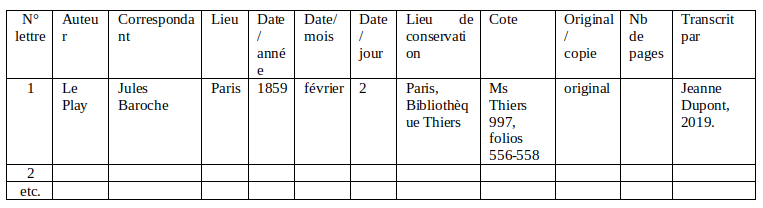
\includegraphics[width=16cm]{images/metadonnees.png}
    \label{metadonnees}
\end{figure}
 
 \subsubsection{Annotation des transcriptions}
 
 Le transcripteur est également chargé de l'annotation, élément clef pour la bonne compréhension et la mise en contexte de la correspondance. Ces notes se font par appel de bas de page et portent sur :
\begin{itemize}
    \item Tous les noms propres cités : avec prénom et nom, dates de naissance et et mort, biographie succinte (deux ou trois lignes maximum).On peut préciser tel élément de contexte permettant de comprendre la relation entre Le Play et son correspondant à ce moment-là.
    \item Tous les noms d'ouvrages cités, avec le titre exact, l'édition citée ou à défaut, la première édition.
    \item Un nom de lieu fautif dans la lettre doit être précisé en note. S’il est fait allusion à un lieu peu connu (village), ou situé à l’étranger, il faut donner la précision nécessaire en note.
    \item Chaque transcripteur, selon son appréciation, annotera tel événement cité, telle référence obscure, trouvant l'équilibre entre trop et trop peu. On peut également indiquer des références bibliographiques, renvoyer à un article.
    \item Une note initiale rappelant l'objet de l'échange peut s'avérer utile.
\end{itemize}
 
 
\subsubsection{Index}
 
Une grande question qui se pose pour l'édition est celle de l'indexation.

Trois index ont été envisagés : 
\begin{itemize}
    \item Un index des noms de personne cités, par ordre alphabétique, et sous la forme suivante :\\
\citecode{Cochin, Augustin (1823-1872)}
\item Un index des lieux cités, sous la forme suivante : \\
\citecode{
Brescia (Italie)\\
Ligoure (Haute-Vienne)\\
Paris}
\item Un index des titres (ouvrages ou revues) cités, sous la forme suivante :\\
\citecode{
\emph{L’Organisation du travail selon la coutume des ateliers et la loi du\\ Décalogue…}, Tours, Mame, 1870.}
\end{itemize}
 
À ces index, nous avons choisi d'ajouter, en accord avec le chef de projet : 
\begin{itemize}
    \item Un index des événements
    \item Un index des noms d'organisation
    \item Un index des termes sociologiques leplaysiens\\
\end{itemize}
 
Tous ces principes de transcription, d'annotation et d'indexation établis par Monsieur Matthieu Brejon de Lavergnée nous ont été très précieux. C'est à eux que nous nous sommes référée pour les adapter ensuite aux possibilités du numérique. Nous y reviendrons donc lorsque nous parlerons de l'acquisition et du traitement des données en indiquant comment transposer en numérique les principes de la correspondance et les choix éditoriaux, selon les outils qui sont à notre disposition.\\

Maintenant que nous avons vu ce qu'impliquait une édition numérique de correspondance, comment concevoir un site adapté à ces exigences ? Nous tenterons de répondre à cette question dans le prochain chapitre.
 
\chapter{Concevoir un site adapté aux exigences de l'édition}

\section{Encoder, oui, mais pourquoi ?}
La conception du site n'a pas été la tâche qui nous a le plus occupée durant nos stages, néanmoins, nous nous sommes un peu penchée sur la question.

Pour ce qui est du projet ELICOM, nous n'avons pas été sollicitée pour cette question fort complexe, d'autant que la plateforme envisagée est assez innovante et pleine de défis.

En revanche, pour le projet d'édition numérique de la correspondance de Frédéric Le Play, au CRHXIX, nous avons été amenée à imaginer le futur site : en effet, un encodage répond à des attentes\footnote{Le principe de l'encodage est davantage expliqué dans la quatrième partie (10.1.1)}. Il est donc nécessaire de savoir ce que l'on veut encoder, mettre en valeur. En effet, on n'encode pas pour encoder mais dans un but précis. Ce chapitre nous aidera donc à avoir une meilleure vue d'ensemble des attentes du site, puisque nous nous penchons ici principalement sur le projet Le Play. \\

Tout d'abord, la mise en contexte par le biais des récits utilisateurs ou \emph{users stories} est un atout précieux. Ceci nous permettra d'élaborer au mieux l'architecture du site, sans oublier le rôle du référencement naturel et la question de la licence.
Ce sont autant de points qui seront développés dans le cahier des charges si l'on envisage une externalisation du projet de développement.

\section{Les récits utilisateurs}

Le but de ce projet, nous l’avons dit plus haut, est de rendre accessible un savoir. Il s’agit véritablement de donner accès aux fonds dispersés de Le Play, afin de favoriser les recherches dans ce domaine et accroître ce savoir sociologique. Pour cela, il est important de pressentir ce que veulent les utilisateurs, quel public nous ciblons, quelles personnes seront intéressées par cette édition numérique et quels seront leurs besoins. 
C’est tout l’intérêt des «\emph{ Users Stories }» ou « récits utilisateurs » de nous éclairer sur ce point. À nous de nous projeter dans la démarche des futurs utilisateurs de notre plateforme.

En effet, \inquote{un récit utilisateur est une phrase simple dans le langage de tous les jours permettant de définir avec suffisamment de précision le contenu d'une fonctionnalité à développer\footnote{\inquote{Récit utilisateur}, \emph{Wikipedia}, Page Version ID 6474167, 2020, URL : \url{https://fr.wikipedia.org/wiki/Recit_utilisateur} (visité le 18/06/2020).}}.

Le récit utilisateur comprend trois éléments principaux : \\
\citecode{En tant que <qui>, je veux <quoi> afin de <pourquoi>}.

Le \citecode{<qui>} est le \emph{persona}, le sujet fictif imaginé. Le \citecode{<quoi>} est le comportement ou fonctionnalité attendue. Le \citecode{<pourquoi>} indique l'intérêt de la fonctionnalité et justifie son développement. 

Inexpérimentée que nous étions dans la pratique des récits utilisateurs, nous avons peiné à créer des récits utilisateurs entièrement satisfaisants et dignes d'être placés dans le corps de ce mémoire. Néanmoins, nous les avons mis dans les livrables, sous forme rédigée dans l'ébauche de cahier des charges et sous forme de tableau dans un fichier excel. Malheureusement, nous n'avons pas pu aller au bout de ce travail, par manque de temps. Cela fait partie d'un des points à retravailler par l'un des membres de l'équipe du CRHXIX pour pouvoir mener à terme le projet.  
	
\section{Élaboration de l'architecture du site}
	
Pour concevoir un site adapté aux exigences de l'édition, outre les récits utilisateurs, il s'agit aussi d'imaginer une architecture du site.

Nous avons également fait une ébauche de cette architecture, la suite sera prise par un membre du CRHXIX plus expérimenté dans ce domaine.
Pour concevoir un site, il est bon d'imaginer le site le plus simple possible, et le plus facile d'utilisation, avec le moins de clics à faire.

Selon les besoins des utilisateurs et pour le succès de notre projet, l’arborescence du site est un élément primordial. Or, l’on ne part pas de rien. Plusieurs sites d’édition numérique de correspondance existent déjà. À nous de nous en inspirer et de les adapter à nos besoins\footnote{La réalisation du site sera probablement confiée à un prestataire.}. 

Pour cela, nous avons pris plusieurs sources d'inspirations, dont deux principales que nous avons déjà évoquées plus haut\footnote{Voir la fin du chapitre 4.} : 
\begin{itemize}
    \item Le site de l'édition numérique de la correspondance de Gustave Flaubert\footnote{\emph{Correspondance, Site web du Centre Flaubert}, URL : \url{https://flaubert.univ-rouen.fr/correspondance/edition/} (visité le 17/06/2020).}.
    \item Celui de la correspondance de Marcel Proust \footnote{\emph{Le Projet, Corr-Proust}, URL : \url{http://proust.elan-numerique.fr/presentation/project} (visité le 08/06/2020).}.
\end{itemize}

Tout d'abord, nous nous sommes inspirée du site d’édition électronique de la correspondance de Gustave Flaubert\footnote{\emph{Accueil}, Site web Centre Flaubert, URL : \url{https://flaubert.univ-rouen.fr/correspondance/edition/}, (visité le 19 juin 2020).}, réalisé par le Centre Flaubert de l’université de Rouen, composante du laboratoire CÉRÉdI (Centre d’Études et de Recherche « Éditer-Interpréter »), et s’inscrivant dans le programme de l’IRIHS (Institut de Recherche Interdisciplinaire Homme et Société), soutenue par Huma-Num, cette « très grande infrastructure visant à faciliter le tournant numérique de la recherche en sciences humaines et sociales \footnote{\emph{Accueil}, Site web d’Huma-Num, URL : \url{https://humanum.hypotheses.org/6089}, (visité le 19 juin 2020).}» et son Consortium Cahier\footnote{\emph{Le Consortium}, Site web OpenEdition, URL : \url{https://cahier.hypotheses.org/le-consortium} (visité le 19 juin 2020)}. 
Sur la page d'accueil de cette édition se trouve le nombre de lettres consultables avec le récapitulatif des lettres écrites par Flaubert et celles qu’il a reçues\footnote{Voir Annexe A.4 }. Est renseignée également une présentation des lettres par ordre chronologique (à la fois par période et par année), par correspondant, par lieu de rédaction et par lieu de conservation. On y voit également un bouton qui dirige vers les thèmes des lettres, un index des noms propres, des cartes du voyage en Orient, et des informations sur l’ancienne édition Louis Conard. Enfin, s’y trouvent toutes sortes de renseignements sur l’édition, tels que les principes de transcription, une présentation de l’équipe, des partenaires et des soutiens. On peut également y faire des recherches, simples ou multicritères, en sélectionnant si c’est une correspondance active ou passive, quel correspondant, quelle période, quel lieu de rédaction nous intéresse, dans quel lieu de conservation se trouve le manuscrit, et enfin, nous pouvons renseigner combien de lettres nous voulons voir apparaître par page, si l’affichage comprend l’incipit, si l’on veut qu’elles soient triées par date.	 

Autant de critères intéressants qui peuvent nous être utiles dans la propre conception de notre édition numérique. Pour notre part, nous pensons retenir la recherche par correspondant, les lieux de rédaction, éventuellement les lieux de conservation.\\

Quant au deuxième site retenu, c’est une édition numérique de la correspondance de Marcel Proust\footnote{\emph{Accueil}, Site web Corr-Proust, URL : \url{http://proust.elan-numerique.fr/}, (visité le 8 juin 2020).}.
Pour chaque lettre au hasard on a la vue numérisée (si elle existe), la transcription, le texte, les notes et les informations\footnote{Voir annexe A.6}. 

Nous pouvons donc partir de ces deux exemples pour voir ce qu’il y a à adapter par rapport à nos besoins. Le point commun à ces deux sites et qui est bien l'objectif de notre édition numérique est le vis-à-vis entre le fac-similé et sa transcription. \\

Nous avons donc imaginé le futur site, de façon assez sommaire, avec ses pages et ses rubriques. Le détail est disponible dans les livrables\footnote{Voir aussi les annexes, figure A.9}.

Il a donc été envisagé d'avoir une page d'accueil\footnote{Il est bon de se référer au document joint dans les livrables intitulé \citecode{architecture\_site\_LP.JPG}} donnant sur sept rubriques : 
\begin{itemize}
    \item \textbf{À propos de Le Play} : c'est une page donnant un minimum d'informations pour les personnes voulant se renseigner sommairement sur Le Play, avec une description de sa vie et de son \oe uvre d'une part, puis une présentation de ses correspondants, et enfin une carte de ses voyages et une visualisation de sa correspondance.
    \item \textbf{Correspondance de Le Play }: cette rubrique présente la correspondance par ordre chronologique (à la fois par période et par année), par correspondant, par lieu de rédaction et par lieu de conservation. En cliquant, on accède à une page présentant la lettre recherchée.
    \item \textbf{Index} : ce terme renferme les six index envisagés\footnote{Nous n'avons pas eu le temps de mettre à jour le fichier \citecode{architecture\_site\_LP.JPG}, mais depuis, la réflexion a continué son cours et d'autres index ont été envisagés lors de l'encodage. En effet, si certaines étapes sont à suivre, elles ne sont pas imperméables, et elles s'enrichissent mutuellement. L'encodage a favorisé une réflexion plus profonde sur l'indexation, permettant de compléter ainsi l'architecture du site.} : tout d'abord, l'index des personnes ou personnages, contemporains de Le Play, historiques ou de fiction, puis l'index des lieux, celui des ouvrages cités, des organisations, des événements évoqués et enfin, particularité de notre correspondance, un index des termes leplaysiens et sociologiques\footnote{Nous y reviendrons lors de la description des choix d'encodage en dernière partie.}. 
    \item \textbf{Recherche} : il sera possible de faire une recherche avancée, par année, éventuellement par plage temporelle comme cela a été fait pour le site \emph{Corr-Proust}, par expéditeur, destinataire, mot, lieu de conservation et lieu de rédaction.
    \item \textbf{Guides }: on aura accès ici à un glossaire, à un recensement des abréviations, et à un guide utilisateur expliquant comment fonctionne le site. 
    \item \textbf{Actualités} : cette page sera à alimenter régulièrement, selon les lettres nouvellement éditées, les modifications, corrections, et ajouts. On pourra profiter de cet onglet pour faire la promotion des événement autour de Frédéric Le Play. Elle aurait l'avantage de permettre un meilleur référencement naturel mais nous reviendrons là-dessus. Il est aussi envisageable de faire une \inquote{Foire aux questions} à cet endroit.
    \item \textbf{À propos de l'édition}. Ici, on pourra voir une présentation du projet, de l'équipe, ainsi que celle de la politique éditoriale, point capital pour garantir la scientificité de l'édition. On présentera aussi les partenaires et soutiens qui appuient également la crédibilité du projet.
\end{itemize}

Enfin, on pourrait envisager d'ajouter un bouton d'\inquote{appel à manuscrits} pour ceux qui possèdent des manuscrits auxquels nous n'avons pas eu accès. En effet, certains manuscrits de Le Play sont en vente sur internet, cela suppose que certains acquéreurs privés doivent en posséder. L'intérêt serait donc, encore une fois, de mettre à la disposition de tous une numérisation et transcription de manuscrits qui dorment dans des lieux oubliés.

On pourrait aussi ajouter un bouton \inquote{Nous contacter} permettant de joindre l'équipe du CRHXIX, pour poser des questions ou proposer des corrections, si l'un des utilisateurs remarque des coquilles qui nous auraient échappées.\\

Ainsi, l'architecture du site est encore en questionnement, mais elle a déjà été envisagée dans sa globalité lors de notre stage.

\section{Le référencement naturel}

Une question que nous nous sommes aussi posée est celle du référencement naturel, autrement dit de l'Optimisation pour les moteurs de recherche ou en anglais \emph{Search Engine Optimization} (SEO). Sur ce sujet, les réflexions ont été à peine ébauchées. Néanmoins, c'est une piste de réflexion que nous ouvrons au CRHXIX : comment faire pour  optimiser le positionnement d'une page ou de notre site dans la page des résultats de recherche d'un moteur de recherche, sachant qu'il s'agit de se trouver dans la première page des résultats du moteur de recherche ou \emph{Search engine result page} (SERP), puisque la plupart du temps, les utilisateurs ne vont pas au-delà :ils cliquent majoritairement sur les cinq premiers résultats de la SERP.
Il faut donc savoir se distinguer parmi les milliers de sites qui existent.

Le SEO est une chose sur laquelle il faut veiller chaque année car les critères varient. Lors donc de la création du site, il faut miser sur une structure du site avec un plan logique et précis\footnote{Voir \emph{SEO et Webdesign : 9 quick wins à intégrer}, Le Marketing aux petits oignons, URL : \url{https://www.emarketing-aux-petits-oignons.com/seo-et-webdesign} (visité le 18/09/2020).}. L'adresse du site ou URL (\emph{Uniform Resource Locator}) doit être court et précis, avec éventuellement des mots-clés. La navigation du site doit être intuitive, et le design doit être \emph{mobile friendly}, autrement dit, il doit être visible sur les appareils à petit écran. La vitesse du site doit être optimale, au risque de perdre des utilisateurs pressés. Les titres, les en-têtes et la balise \emph{meta description} doivent être bien pensés ; chaque page doit être composée d'un contenu unique dans son intitulé, avec des mots-clés relatifs à son contenu. Il faut également optimiser les images dans leur description. Les images trop grandes risquent de réduire la vitesse de téléchargement du site, ce sera donc un défi à relever pour notre site. En effet, on remarque sur certains sites d'édition numérique de correspondance, les images sont parfois un peu longues à charger. Un \emph{design} attrayant est un plus et dans notre cas, cela nous permettra peut-être d'avoir un public plus large que les simples chercheurs qui savent pourquoi ils ont fait cette requête et resteront sur le site même s'il n'est pas attractif, intéressés qu'ils sont par son contenu intellectuel. 
Enfin, la page d’accueil est \inquote{en général la page la plus forte d’un site : plus une page est éloignée de la page d’accueil, plus il est difficile pour elle d’être correctement référencée\footnote{\emph{Optimiser  l’architecture d’un site web pour le SEO}, Site web La Fabrique du Net, URL : \url{https://www.lafabriquedunet.fr/seo/articles/optimiser-architecture-site-web-seo/}, (visité le 25 juin 2020).}.} Il faudra donc prendre en compte tous ces principes pour garantir le bon classement de notre site sur le Web et gagner l'une des premières places sur la SERP afin d'avoir une audience conséquente.

\section{La licence ou le cadre juridique}

Un publication va de pair avec le choix d'une licence. Il est nécessaire d'associer une licence à nos jeux de données. La licence encadre et sécurise les réutilisations des données permises par le titulaire des droits d'auteur\footnote{Gauthier Poupeau, \emph{Open Data, Big data, Data Mining,}Module data, M2 TNAH ENC, Cours 2, 21 octobre 2019. La figure 6.1 est tirée de ses slides.}. Leur choix est vaste, comme le souligne la description ci-dessous :

\begin{figure}[ht]
    \centering
    \caption{Les licences}
    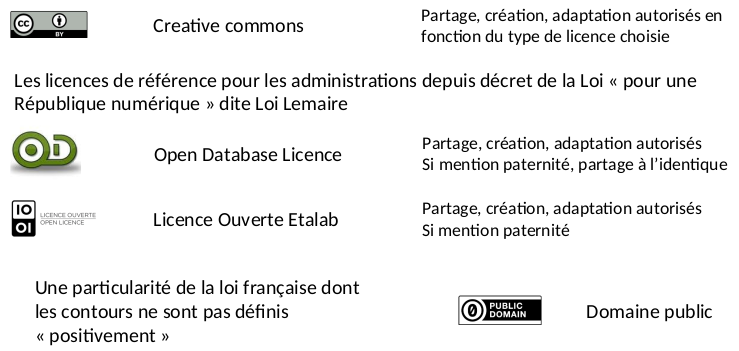
\includegraphics[width=16cm]{images/licences.png}
    \label{licences}
\end{figure}

ELICOM part sur une licence \citecode{CC BY-NC-ND 3.0 FR} : c'est une licence \citecode{Creative commons}, qui autorise à partager, copier, distribuer et communiquer le matériel par tous moyens et sous tous formats. L'offrant ne peut retirer les autorisations concédées par la licence tant que les termes de cette licence sont appliqués\footnote{\emph{Creative commons}, CC BY-NC-ND 3.0 FR, URL : \url{https://creativecommons.org/licenses/by-nc-nd/3.0/fr/} (visité le 18/09/2020).}. Quatre conditions entrent en ligne de compte : on doit mentionner d'une part d'où viennent les informations, de plus, on n'est pas  autorisé à faire un usage commercial de l'\oe uvre ni de modifications, ni de restrictions complémentaires.
L'utilisateur n'est pas dans l'obligation de \inquote{respecter la licence pour les éléments ou matériel appartenant au domaine public ou dans le cas où l'utilisation [...] est couverte par une exception}\footnote{\emph{Idem.}}.

\section{Le cahier des charges}

Finalement, la clef pour concevoir un site adapté aux exigences de l'édition se trouve dans le cahier des charges.
Celui-ci permet d'exprimer les attentes de l'édition et garantit une mise en pratique planifiée et réaliste. 

Pour ce qui est des projets numériques, on constate que les deux tiers rencontrent de gros problèmes et un tiers se solde par un échec. Cette proportion est stable en France et dans les autres pays du monde, et aussi bien dans le public que le privé\footnote{Voir Jean-Louis Foucard, Module de formation
\inquote{Manager un projet Numérique} Master \inquote{Archives – Technologies numériques appliquées à l’histoire}, École Nationale des Chartes, mars 2020.}.

Une des raisons se trouve dans le flou qui règne autour des projets, l'irréalisme, les imprécisions, l'inadéquation entre les objectifs et les moyens.
Or, le cahier des charges est ainsi nommé car, à sa lecture, on peut estimer
les charges. Il est un pont entre celui qui a le besoin et celui qui le résout. 

Il présente à la fois le contexte du projet, ses objectifs, son périmètre, les besoins en terme de fonctionnalités, les ressources disponibles et les contraintes pour la réalisation du projet, le budget et les délais qui permettent au prestataire d’évaluer la durée de travail et de s’organiser\footnote{\emph{Exemple cahier des charges}, CahiersDesCharges.com, URL : \url{https://cahiersdescharges.com/exemple-cahier-des-charges-pdf/} (visité le 12/06/2020).}.\\

Le Labex OBVIL avait déjà établi un cahier des charges du projet il y a deux ans. Celui-ci nous a bien aidée pour définir les priorités et choisir les correspondances à traiter, de la plus facile à la plus difficile.

Pour le CRHXIX, le cahier des charges reste encore à faire. Nous voulions y résumer l'ensemble de nos attentes pour le futur site : comment voulons-nous que le site soit configuré ? Quelles fonctionnalités désirons-nous ? Nous y avons travaillé mais le résultat est encore entre un rapport et une ébauche de cahier des charges\footnote{Voir dans les livrables.}. En effet, pour établir un cahier des charges, il faut compter un certain nombre de jours de travail, et nous n'avons travaillé qu'une petite trentaine de jours au CRHXIX. Nous avons donc dû passer assez rapidement à la suite, c'est-à-dire à la partie d'acquisition et de traitement des données. Néanmoins, les réflexions que nous avons été amenée à faire sur le cahier des charges nous ont bien éclairée pour la suite, en témoigne ce présent chapitre sur la conception d'un site adapté à l'édition numérique de correspondance.\\

Une fois l'édition pensée, il s'agit de mettre en pratique. Ceci se fait en deux temps. Il s'agit tout d'abord d'acquérir les données (partie III) puis de les traiter (partie IV). Or, l'apprentissage machine joue un grand rôle aujourd'hui dans l'acquisition des données. C'est ce point que nous aborderons dans la partie suivante. 

   

\part{L'apprentissage machine au c\oe ur de l'acquisition des données}

\begin{figure}[ht]
    \centering
    \caption{Processus de travail d'encodage}
    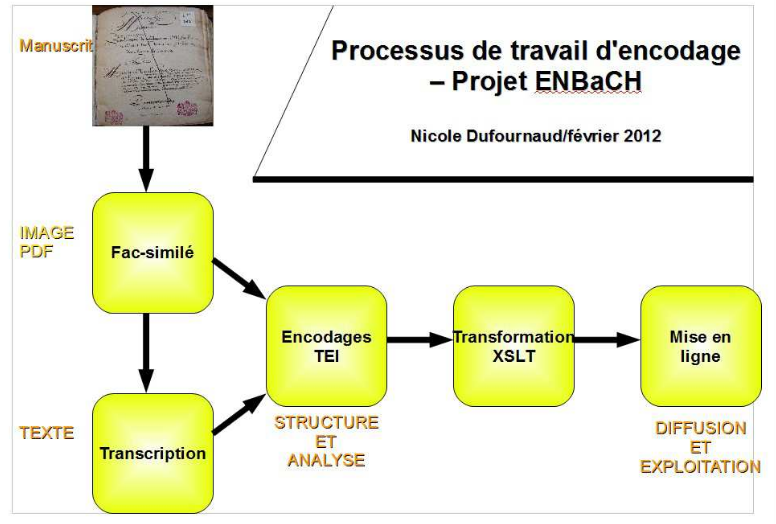
\includegraphics[width=16cm]{images/processus_encodage.png}
    \label{processus_encodage}
\end{figure}

La suite de ce mémoire va être consacrée à l'acquisition et au traitement des données. Nous avons trouvé ici un schéma qui éclaire en partie le processus qui amène à la mise en ligne des données. Même si celui-ci diffère selon les projets, on observe de grandes constantes.

Tout d'abord, il y a la donnée brute~: le manuscrit. C'est le cas pour le projet Le Play. Pour ELICOM, nous avons à faire à une édition papier imprimée. Après le manuscrit suit l'image numérisée, dont on se sert pour faire les transcriptions - c'est la partie acquisition des données - et à partir de là, l'encodage en TEI. On peut avoir recours à une transformation XSLT (\emph{Extensible Stylesheet Language Transformations}), on parlera rapidement de cette éventualité. Et enfin, la mise en ligne, objectif de nos projets pour leur diffusion et exploitation. Puisse ce schéma éclairer les propos qui suivront. 

\chapter{L'apprentissage machine}

\section{Petite histoire de l'apprentissage machine}

Pour mieux comprendre ce qui va suivre, il importe de revenir sur ce qu'est l'apprentissage machine afin de mieux saisir en quoi il intéresse nos projets.

Le terme \emph{Machine Learning} (ML), traduit en français par \inquote{apprentissage machine} ou encore \inquote{apprentissage automatique}, est apparu pour la première fois dans la bouche d'Arthur Samuel, en 1959, un pionnier américain dans le domaine des jeux vidéo et de l'intelligence artificielle. Il évoque la possibilité qu'a la machine d'apprendre sans être vraiment programmée\footnote{\emph{An introduction to Machine Learning}, Site web GeeksforGeeks, URL~: \url{https://www.geeksforgeeks.org/introduction-machine-learning/} (visité le 20/09/2020). }.

En effet, la machine peut être programmée pour apprendre de son expérience. On verra très nettement par la suite qu'elle fait, pour ainsi dire, des progrès. Elle apprend une écriture, à travers des \inquote{\emph{features\footnote{Une des techniques de reconnaissance est la \inquote{classification par caractéristiques (\emph{features}) : une forme à reconnaître est représentée par un vecteur de valeurs numériques - appelées \emph{features} en anglais - calculées à partir de cette forme}. Voir \emph{Reconnaissance optique de caractères}, Wikipedia, URL : \url{https://fr.wikipedia.org/wiki/Reconnaissance_optique_de_caracteres} (visité le 30/09/2020).}}}, et plus on lui donne de lettres à apprendre, plus elle progresse, jusqu'à pouvoir faire la transcription elle-même en prédisant le caractère à reconnaître par rapport à ce qu'elle a appris, avec un taux de réussite plus ou moins important\footnote{L'apprentissage machine a plusieurs divisions comme l'apprentissage supervisé ou non supervisé, ou encore l'apprentissage par renforcement et l'apprentissage semi-supervisé. Mais nous ne rentrons pas ici dans les détails de l'algorithme.}. 

\section{Apprentissage machine et intelligence artificielle}

Comme nous l'avons rapidement souligné, l'apprentissage machine est une composante de l'intelligence artificielle (IA). Celle-ci est la \inquote{recherche de moyens susceptibles de doter les systèmes informatiques de capacités intellectuelles comparables à celles des êtres humains}\footnote{\emph{La Recherche}, janv. 1979, n.96, vol. 10, p. 61}. Elle se traduit par  « l'ensemble des théories et des techniques mises en œuvre en vue de réaliser des machines capables de simuler l'intelligence »\footnote{\emph{Intelligence artificielle}, Wikipédia, URL~: \url{https://fr.wikipedia.org/wiki/Intelligence_artificielle} (visité le 20/09/2020).}. C'est une capacité d'un programme informatique à fonctionner comme un cerveau humain. Elle utilise, avec les réseaux de neurones la façon de fonctionner de l'intelligence humaine. Ainsi, on voit que le fait qu'une machine puisse apprendre et faire en quelque sorte des progrès fait partie de l'IA. Le schéma ci-dessous\footnote{Gauthier Poupeau, \emph{Open Data, Big data, Data Mining,}Module data, M2 TNAH ENC, Cours 2, 21 octobre 2019} permet de comprendre davantage la place du \emph{Machine Learning} dans l'IA. On voit que l'apprentissage machine et l'apprentissage profond ou \emph{deep learning} sont des sous-ensemble de l'IA. Cependant, ils ne sont pas l'IA mais un moyen de parvenir à l'IA un jour. 

\begin{figure}[ht]
    \centering
    \caption{\emph{Machine learning} et IA}
    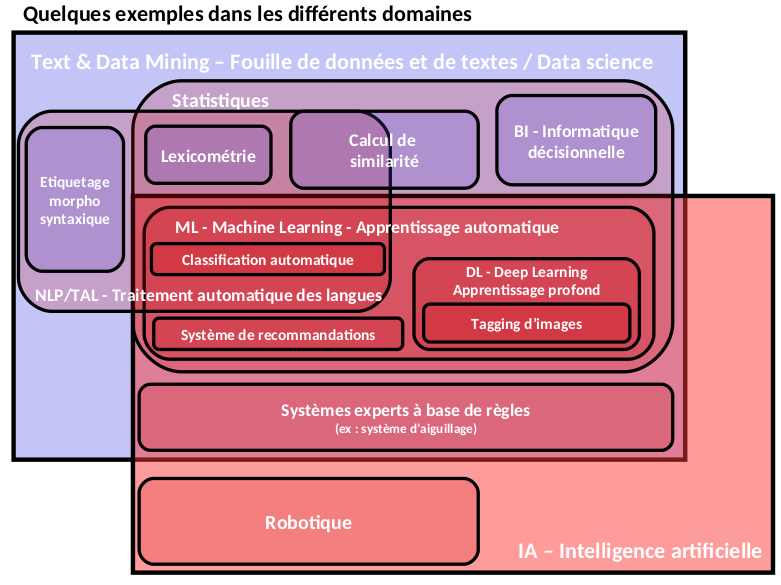
\includegraphics[width=16cm]{images/ia_poupeau.png}
    \label{ia_poupeau}
\end{figure}


Ainsi, pour distinguer \emph{machine learning} et \emph{deep learning}, on peut dire que le \emph{machine learning} est un \inquote{système visant à accomplir des tâches à partir de caractéristiques et attributs communs (patterns) ``appris'' dans un ensemble de données d'exemples}\footnote{\emph{Idem}, p. 27}~: la machine apprend les données et les applique de la bonne façon ; tandis que le \emph{deep learning} est un sous-ensemble du \emph{machine learning}, une \inquote{technique d’apprentissage cherchant à reproduire le mécanisme des réseaux de neurones du cerveau humain}\footnote{\emph{Ibidem.} p. 28}. Il est plus poussé, plus abouti et plus autonome\footnote{Voir \emph{Artificial intelligence vs Machine Learning vs Deep Learning}, Site web Geeksforgeeks, URL~: \url{https://www.geeksforgeeks.org/artificial-intelligence-vs-machine-learning-vs-deep-learning/?ref=rp} (visité le 20/09/2020).}.

Ainsi, nous verrons que les technologies que nous utiliserons de \emph{machine learning} ne sont pas encore abouties et nécessiteront un traitement conséquent. 

\section{L'apprentissage machine dans nos deux projets}

Lorsqu'on a une quantité de lettres à éditer de façon numérique, comment utiliser au mieux les capacités de la machine pour qu'elle nous aide dans l'acquisition des données ?
C'est tout le rôle de l'apprentissage machine qui permet une reconnaissance automatique des caractères et permet la transcription des textes. Or, nous sommes ici face à deux types de textes~: pour ELICOM, nous avons des éditions papier numérisées et disponibles sur Gallica, qui ont été imprimées. Ce sont des caractères d'imprimerie. Pour l'édition numérique de la correspondance de Frédéric Le Play, ce sont des manuscrits écrits au moins de moitié si ce n'est majoritairement de la main de Le Play. Ce sont donc des caractères d'écriture manuscrite. À chaque projet corrrespond donc une technologie différente. Pour les caractères d'imprimerie, on parlera d'\emph{Optical Character Recognition} ou Reconnaissance optique de caractères (OCR), pour la reconnaissance de l'écriture manuscrite, on parlera d'\emph{Handwritten Text Recognition} (HTR). \\

Ainsi, l'OCR\begin{quote}
    \inquote{désigne le processus informatique qui vise à transposer des éléments textuels présents sur une image numérique vers un fichier de texte de manière automatique. Il s'agit, en d'autres termes, de faire réaliser par l'ordinateur la tâche de copie du texte\footnote{Alix Chagué, \emph{Constituer un corpus pour la fouille de texte - de la transcription des documents d’archives à l’annotation~: exploration d’une méthodologie par l’ANR Time Us}, mémoire de master « Technologies numériques appliquées à l’histoire », dir. Vincent Jolivet et Éric de la Clergerie, École nationale des
chartes, 2018, p.41.}.
}
\end{quote}

L'OCR de Gallica est un service qui permet la reconnaissance de texte dans une image\footnote{\emph{Mode texte et OCR}, Site web BNF.Gallica, URL~: \url{https://gallica.bnf.fr/edit/und/consulter-les-documents} (visité le 21/09/2020).}. Ainsi, le contenu des documents numérisés est extrait et transformé en fichier texte. Gallica propose le téléchargement au format \citecode{.txt} du résultat de l'OCR. Néanmoins, il ne s'agit pas de texte brut mais d'un texte semi-structuré via des balises \emph{Hypertext Markup Language} (HTML), langage de balisage conçu pour représenter les pages web. Le texte étant ainsi structuré par les balises, on peut ensuite le transformer plus facilement en vue de notre édition. Nous y reviendrons. Le service de Gallica a donc été très précieux pour notre projet d'ELICOM. \\ 

Quant à l'édition numérique de la correspondance de Frédéric Le Play, nous nous sommes servie de l'HTR via Transkribus, qui permet de transcrire cette fois l'écriture manuscrite, grâce à l'entraînement d'un modèle par main. \\

Ainsi, l'apprentissage machine est au c\oe ur de l'acquisition des données pour nos deux projets. Il est temps de voir cela plus en détail, avec l'OCR et l'HTR.



\chapter{L'OCR de Gallica}

\section{Un service à ne pas négliger}
\subsection{Un OCR plutôt fiable}
Pour le projet ELICOM du Labex OBVIL, nous avons beaucoup exploité l'OCR de Gallica.
En effet, les textes que nous avons extraits sont issus d'un traitement OCR brut, sans relecture, que nous relirons sommairement par la suite. La qualité (taux OCR) dépend de l'état de la source, de la langue, mais aussi de la campagne de numérisation\footnote{C'est la même chose que pour le projet de la Très grande bibliothèque (TGB) mené aussi par OBVIL, voir~: \emph{TGB (BnF – OBVIL)}, Site web provisoire TGB, OBVIL et BNF, URL~: \url{http://obvil.lip6.fr/tgb/} (visité le 08/09/2020).}. Certains livres numérisés avaient par exemple des marques de crayon de papier, ce qui est parfois mal interprété par l'OCR. 
En effet, \begin{quote}
    \inquote{Même si les techniques d'OCR sont en progrès constant, la qualité de reconnaissance dépend malgré tout d'un grand nombre de facteurs liés tant au document original qu'à la numérisation elle-même. Ainsi les documents patrimoniaux de Gallica présentent un certain nombre de défis pour l’OCR~: dégradation du papier ou de l’encrage, polices de caractères ou orthographes anciennes, etc. De plus, les anciens modes de numérisation (en noir et blanc, d’après microfilm) ont un impact négatif sur les performances\footnote{\emph{Mode texte et OCR}, Site web BNF.Gallica, URL~: \url{https://gallica.bnf.fr/edit/und/consulter-les-documents} (visité le 21/09/2020).}.}
\end{quote}
Certains textes ont cependant un taux avancé d’OCR de 100\%. Cependant, un taux de 100\% ne signifie pas un sans fautes. De toutes façons, une relecture précise et attentive sera toujours nécessaire même sur un texte dont le taux est déclaré de 100\%. 
En effet, 
\begin{quote}
    \inquote{Ces estimations donnent généralement un bon aperçu de la qualité globale d’un document, mais elles ne doivent pas être confondues avec le taux qualité réel,  qui ne peut être connu (sauf à corriger le texte d’un document et comparer cette référence avec le texte OCR, ce qui est impossible dans un contexte de numérisation de masse).
De plus, ces indicateurs ne sont pas toujours calculés à partir de la totalité du document ; il se peut par exemple que des zones illisibles ou trop complexes soient exclues du calcul et que la qualité perçue par le lecteur soit ainsi très nettement inférieure à la qualité annoncée\footnote{\emph{Idem.}.}}
\end{quote}

L'avantage que représentent les imprimés du XIX\up{e} siècle est leur relative modernité~: ils sont à la fois suffisamment anciens pour être libres de droits, contrairement aux imprimés des XX\up{e} et XXI\up{e} siècle, et ils ont aussi l'avantage d'être relativement modernes dans leur typographie, donc mieux reconnus automatiquement que les imprimés plus anciens qui comportent souvent des \inquote{s} longs ou autres caractéristiques qui sont autant d'obstacles pour l'OCR et nuisent à sa qualité.

Comme nous l'avions souligné lors de la présentation des sources\footnote{Voir 3.2}, nous avons choisi les correspondances à traiter en priorité d'une part en fonction des marqueurs du texte qui garantissent une extraction plus aisée, d'autre part en fonction de la qualité de l'océrisation. 
Or, la correspondance d'Alphonse de Lamartine semblait réunir ces deux avantages~: pour ce qui est de l'extraction, elle était classée \inquote{relativement facile grâce aux chiffres romains qui délimitent les lettres} dans le cahier des charges, et l'OCR de Gallica indiquait un taux de réussite estimé à 100\%. Nous avons donc choisi de commencer par là notre travail d'extraction et d'acquisition des données. Puis nous nous sommes concentrée sur la correspondance de Félicité de Lamennais pour finir ensuite sur celle de Pierre-Joseph Proudhon. 

Une question s'est posée assez rapidement~: devons-nous systématiquement utiliser le service OCR de Gallica ou est-il opportun de passer par un autre moyen pour extraire le texte, comme par exemple Transkribus ou un équivalent. Nous avons donc demandé conseil à des personnes expertes en la matière. À cela il nous a été répondu que l'OCR de Gallica est un service à ne pas négliger, et comme vu plus haut, les taux de réussite étant relativement bons, il nous a paru plus intéressant de l'exploiter au maximum, d'autant que nous ne sommes pas intéressés par une correspondance entre l'image et le texte, étant donné que nous ne mettrons en ligne que le texte extrait et non l'image de la première édition papier. 

Revenons donc sur cette phase d'acquisition et de pré-traitement des données. Celle-ci s'est faite en plusieurs étapes. 

\subsection{Extraction de l'OCR en HTML}

Pour acquérir les données, il s'agit de les extraire. Cela a occupé la première phase de notre travail. 
Pour chacun des auteurs sélectionnés, nous sommes allés sur le catalogue général de la BNF qui nous a redirigé vers la page de Gallica permettant de télécharger la correspondance sous trois formats~: soit PDF (\emph{Portable Document Format}), soit JPEG (\emph{Joint Photographic Experts Group}), ou encore TXT (fichier texte). Nous avons choisi cette dernière option. En téléchargeant l'OCR en fichier texte brut.
En effet, cela permet d'une part de s'assurer de la qualité de l'océrisation~: au début de chaque fichier TXT extrait se trouve un récapitulatif sur le document et ses métadonnées essentielles, et une phrase générée automatiquement elle aussi donnant des précisions sur l'OCR. Ainsi, pour la correspondance de George Sand, on peut lire que \inquote{Le texte affiché peut comporter un certain nombre d'erreurs. En effet, le mode texte de ce document a été généré de façon automatique par un programme de reconnaissance optique de caractères (OCR). Le taux de reconnaissance estimé pour ce document est de 96~\%.} L'OCR est ici brute~: elle n'a pu être relue. Ces erreurs sont repérées par des caractères gris pâles au lieu des caractères noirs.

\begin{figure}[ht]
    \centering
    \caption{L'OCR de George Sand sous format TXT}
    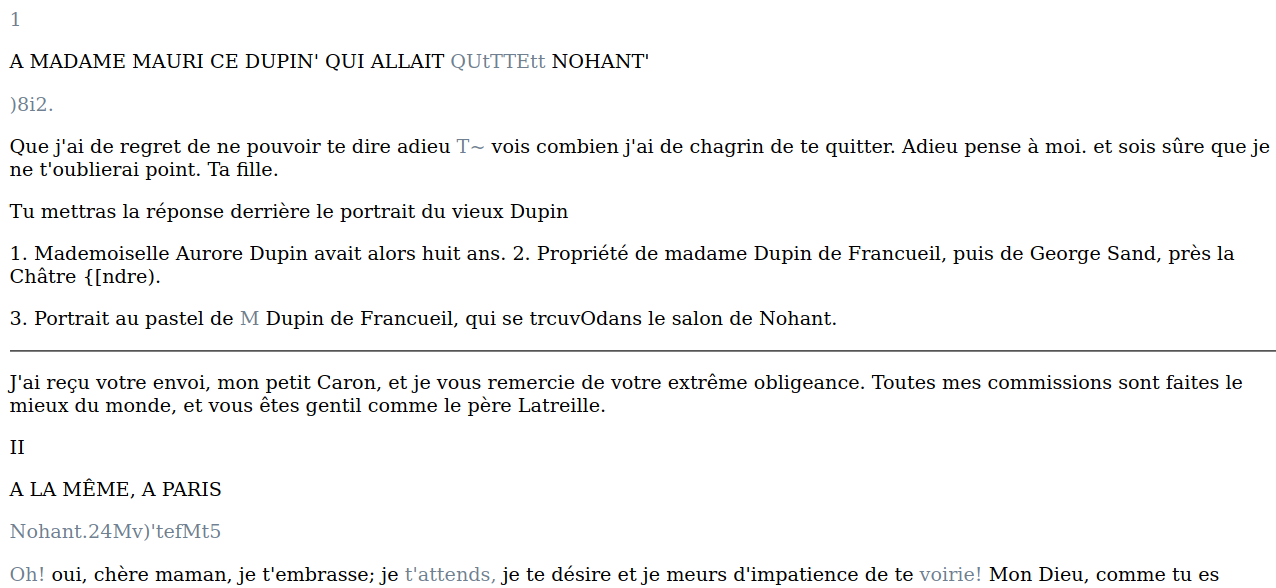
\includegraphics[width=16cm]{images/sand-ocr.png}
    \label{sand-ocr}
\end{figure}

Ainsi, pour le premier volume de la correspondance de George Sand\footnote{\emph{Correspondance~: 1812-1876. George Sand}, BNF.Gallica, URL~: \url{https://gallica.bnf.fr/ark:/12148/bpt6k2065433/f1n385.texteBrut} (visité le 19/05/2020).}, on constate ici des mots grisés~: ce sont toutes les mots soupçonnés d'avoir été mal lu par la reconnaissance automatique. La machine indique donc qu'elle estime s'être trompée sur ces parties. Et effectivement, on peut lire qu'il est écrit \inquote{)8i2.} au lieu de \inquote{1812}, ou encore \inquote{T~} au lieu de \inquote{Tu}. 
Cependant, on voit aussi que certaines parties en noir, et donc présumées justes, sont en réalité fausses~: ainsi il est écrit \inquote{\{[ndre)} au lieu de \inquote{(Indre)}~: la parenthèse ouvrante a été remplacée par une accolade ouvrante, et le \inquote{I} majuscule a été remplacé par un crochet ouvrant. On a donc ici une illustration des limites de l'OCR.

Mais que faire avec ce texte brut ? Il ne nous intéresse pas particulièrement. Il s'agit donc d'extraire le code source sous le format HTML. 

HTML est le langage informatique de base d'Internet, utilisé pour la mise en forme des pages Web\footnote{Depuis 2014, on en est à la version HTML5. Voir~: \emph{HTML (HyperText Markup Langage)~: définition, traduction}, Site web JDN, URL~: \url{https://www.journaldunet.fr/web-tech/dictionnaire-du-webmastering/1203255-html-hypertext-markup-langage-definition-traduction/} (visité le 21/09/2020).}. Il repose sur un système de balises, d'où son nom qui signifie \inquote{langage de balisage d'hypertexte}. 
Comme pour XML, les balises vont toujours par deux, une ouvrante (pour un paragraphe, ce sera \citecode{<p>}), une fermante (\citecode{</p>}).
 La balise ouvrante peut avoir un attribut pour qualifier l'élément.

En extrayant l'OCR sous le format HTML, l'avantage est d'avoir un texte déjà structuré. On peut le constater ci-dessous avec l'exemple de l'OCR de Lamartine au format HTML, avec l'éditeur XML Oxygen XML Editor. Chaque part de texte signifiant - comme la ligne de la date, le salut, le paragraphe - est encadré par une balise \citecode{<p>} indiquant que c'est un paragraphe ou du moins une division particulière. Par ailleurs, les métadonnées sont comprises dans une balise \citecode{head}, elle-même embrassant des balises \citecode{<meta>} contenant des attributs comme \citecode{@name} ou \citecode{@content}.
Le corps du texte quant à lui est contenu dans une balise \citecode{<body>}. Les balises \citecode{<span>} indiquent les erreurs de l'OCR.

\begin{figure}[ht]
    \centering
    \caption{L'OCR de Lamartine en HTML sous Oxygen XML Editor}
    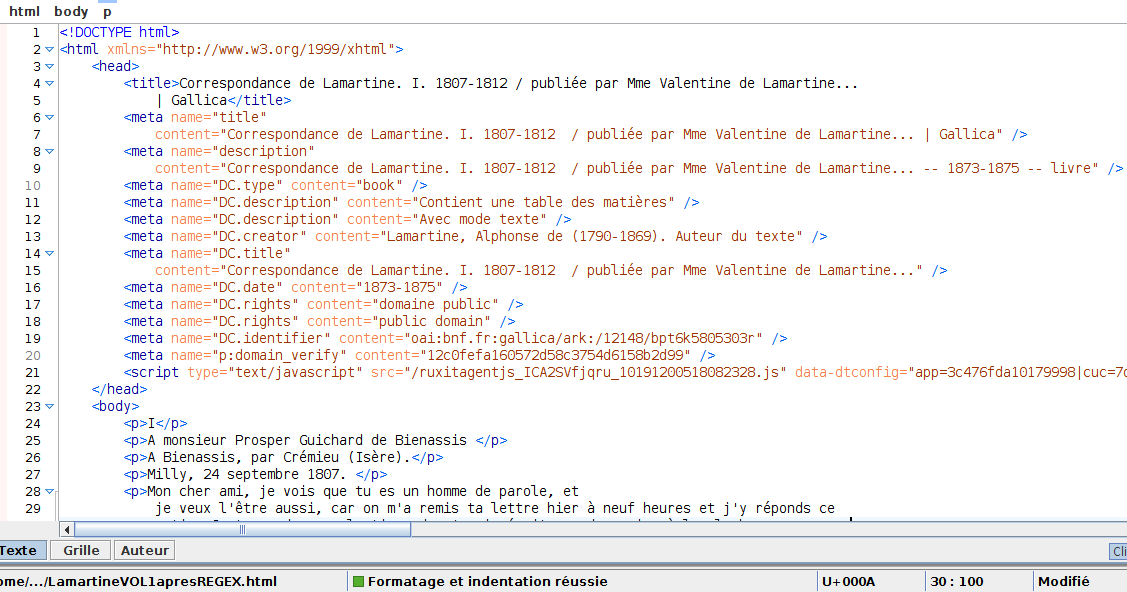
\includegraphics[width=16cm]{images/lamartine_html.png}
    \label{lamartine_html}
\end{figure}

Le texte est donc bel et bien structuré et cela nous permettra par la suite de le transformer plus facilement en XML. En attendant, l'OCR extrait en HTML est loin d'être parfait. L'illustration présente (figure 8.2) montre l'HTML tel qu'il est après correction. En effet, toute une phase de pré-traitement s'est avérée être nécessaire avant de passer à l'étape de transformation en XML que nous développerons dans la quatrième partie de notre mémoire.


\section{Un pré-traitement qui suscite des questionnements}

\subsection{Rendre l'HTML valide et bien indenté}

Notre premier souci lors du téléchargement de l'OCR en HTML a été de vérifier la validité et la bonne indentation de notre fichier HTML. Or, les différents fichiers extraits de Gallica présentaient tous des erreurs dans les balises~: les balises \citecode{<meta>} n'étaient pas fermées et il était donc impossible d'indenter le texte correctement. De même pour les balises \citecode{<br>} (élément de saut de ligne) et \citecode{<hr>} (pour \emph{horizontal rule}, règle horizontale servant de séparation, elles indiquent ici les changements de page, on en trouve donc 391 occurences pour Lamartine). Nous avons donc commencé par fermer toutes ces balises\footnote{Avec la nouvelle version d'Oxygen XML Editor, cela peut se faire de façon automatique.}. Nous avons également choisi de supprimer les ensembles de balises \citecode{</p><hr/><p>} (40 occurences dans Lamartine) et \citecode{</p><p>} (58 occurences dans Lamartine) quand elles divisaient des phrases, étant donc inopportunes et rompant par là l'unité. De même, les titres courants, figurant en en-tête sont des informations superflues. Fort heureusement, elles ont été supprimées automatiquement par l'OCR pour la correspondance de Lamennais (en effet, on lisait « CORRESPONDANCE » à la page de gauche, « DE LAMENNAIS » à la page de droite), ne polluant donc pas l’HTML, contrairement à Lamartine où l'OCR de Gallica ne les avait pas supprimés.

Ensuite, même si cela n'était pas absolument nécessaire, nous avons supprimé tout ce qui concernait les rappels de la demande, les tables des matières et préfaces. Nous aurions aussi pu le faire en amont, lors du téléchargement.
Ainsi, l’HTML de Lamennais comporte 12 204 lignes au départ, 8680 après nettoyage (soit le double de l’HTML de Lamartine après nettoyage). 

Nous avons donc désormais un HTML valide et bien indenté. Cependant, des fautes subsistent.

\subsection{Quelques fautes de l'OCR, visibles dans l'HTML}

Nous avons vu plus haut que certaines fautes étaient grisées dans l'OCR en format TXT. Ceci se retrouve donc logiquement dans l'OCR en format HTML, avec les balises \citecode{<span>}. Or, on remarque que celles-ci sont parfois utilisées à bon escient, tandis que d'autres fois, elles sont absentes ou superflues.

Les balises \citecode{<span>} indiquant les doutes sur l’OCR sont absentes dans la correspondance de Lamartine. En revanche, on en trouve 510 ouvrantes et fermantes dans le premier volume de correspondance de Lamennais. C'est pour les erreurs quasiment avérées, mais beaucoup d’autres erreurs se sont glissées dans le texte, sans être signalées par une balise.  Une relecture sera donc nécessaire. 
Ainsi, à la ligne 7805 du fichier HTML de Lamennais, on voit une faute mentionnée dans une balise \citecode{<span>}, avec un attribut \citecode{@style} pour qu'il apparaisse en gris, comme on peut le constater dans la figure ci-dessous.

\begin{figure}[ht]
    \centering
    \caption{Exemple d'une balise \citecode{<span>} dans l'HTML du premier volume de Lamennais, l. 7805}
    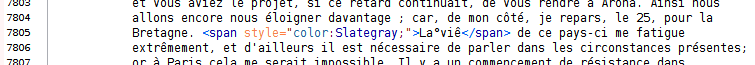
\includegraphics[width=16cm]{images/span_lamennais_7805.png}
    \label{span_lamennais_7805}
\end{figure}

Cependant, certaines fautes ne sont pas signalées par l'OCR, comme on peut le constater vingt lignes plus loin dans le même fichier.

\begin{figure}[ht]
    \centering
    \caption{Exemple d'une balise \citecode{<span>} manquante dans l'HTML du premier volume de Lamennais, l. 7825}
    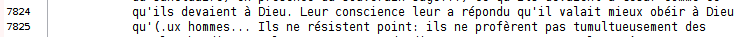
\includegraphics[width=16cm]{images/sans_span_lamennais.png}
    \label{sans_span_lamennais}
\end{figure}
Ici, le \inquote{a} est remplacé par une parenthèse ouvrante et un point. 

Enfin, parfois, les balises \citecode{<span>} sont présentes alors qu’aucune faute n’est à signaler, comme par exemple à la ligne 1264 où le guillemet est juste alors que signalé comme douteux, comme on peut le constater ci-dessous. 

\begin{figure}[ht]
    \centering
    \caption{Exemple d'une balise \citecode{<span>} superflue dans l'HTML du premier volume de Lamennais, l. 1264}
    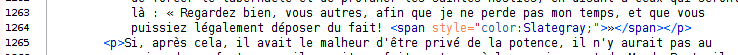
\includegraphics[width=16cm]{images/span_inutile_lamennais.png}
    \label{span_inutile_lamennais}
\end{figure}



\subsection{L'apport des expressions régulières dans le nettoyage de l'HTML}

L'idéal aurait été de toucher le moins possible à l'HTML et de ne faire que des traitements applicables à tous les autres volumes d'un même correspondant. 

Cependant, nous avons procédé tout de même à un nettoyage sommaire de l'HTML. Pour cela, les expressions régulières nous ont été un outil précieux. On entend par \inquote{expressions régulières} ou \inquote{regex}, de l'anglais \emph{regular expression}, une chaîne de caractères, qui décrit, selon une syntaxe précise, un ensemble de chaînes de caractères possibles. En l'utilisant dans un éditeur de texte, ou sinon dans Python, on peut ainsi \inquote{matcher}, c'est-à-dire sélectionner certaines suites de chaînes de caractères récurrentes et les sélectionner toutes ensemble, puis soit les remplacer par une autre chaîne de caractère, soit les supprimer définitivement. C'est donc très précieux pour faire des modifications dans les textes, et ici pour pré-traiter notre HTML.

Comme nous l'avons déjà évoqué plus haut, certains titres dans Lamartine polluaient le texte, comme on peut le constater dans la figure suivante~: tous les éléments inutiles y sont surlignés en jaune.

\begin{figure}[ht]
    \centering
    \caption{Exemple des titres polluant le texte, HTML de Lamartine}
    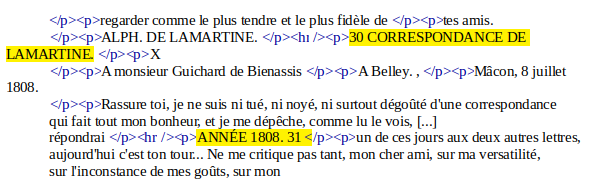
\includegraphics[width=16cm]{images/titres_lamartine.png}
    \label{titres_lamartine}
\end{figure}

Avec l'éditeur de texte Oxygen XML Editor, nous pouvons user des regex. C'est donc par ce biais que nous avons supprimé ces titres. 

\begin{figure}[ht]
    \centering
    \caption{Exemple d'une regex pour enlever certains titres, HTML de Lamartine}
    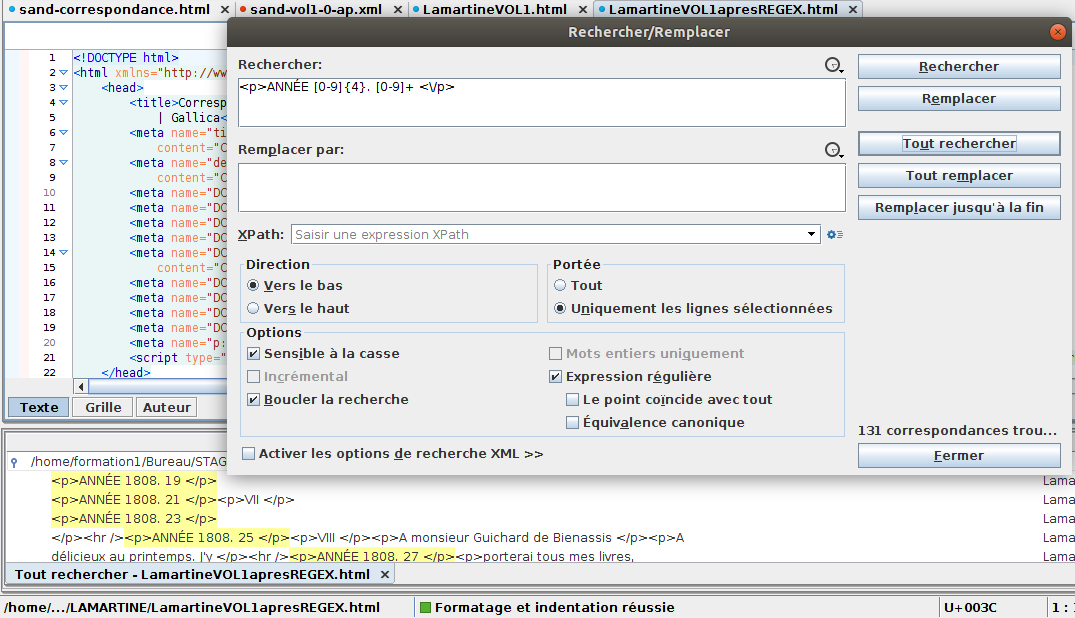
\includegraphics[width=16cm]{images/titres_annee_lamartine.png}
    \label{titres_annee_lamartine}
\end{figure}

La capture d'écran ci-dessus montre comment cela se présente~: on indique dans la fenêtre la regex, et en cliquant sur \inquote{tout rechercher}, 131 matches sont renseignés. Il suffit ensuite d'indiquer \inquote{tout remplacer} et l'HTML est donc nettoyé des 131 titres superflus. 

Malheureusement, nous ne pouvons trouver des regex applicables à tous les corpus étant donné qu'ils se présentent différemment. Ainsi, pour la correspondance de Proudhon, nous supprimons ces titres avec une regex qui diffère~: \citecode{<p>[0-9]\{1,3\} CORRESPONDANCE <\/p>}. Elle fait 108 matches.

De même, pour supprimer les \citecode{</p><p>} évoqués plus haut et coupant les phrases en deux, rompant ainsi l'unité, nous avons également utilisé les regex, cette fois-ci en indiquant que nous ne voulions supprimer que les \citecode{<p>} englobant des minuscules, car minuscules signifient phrases en cours.

\begin{figure}[ht]
    \centering
    \caption{Exemple d'une regex pour enlever des \citecode{<p>}, HTML de Lamartine}
    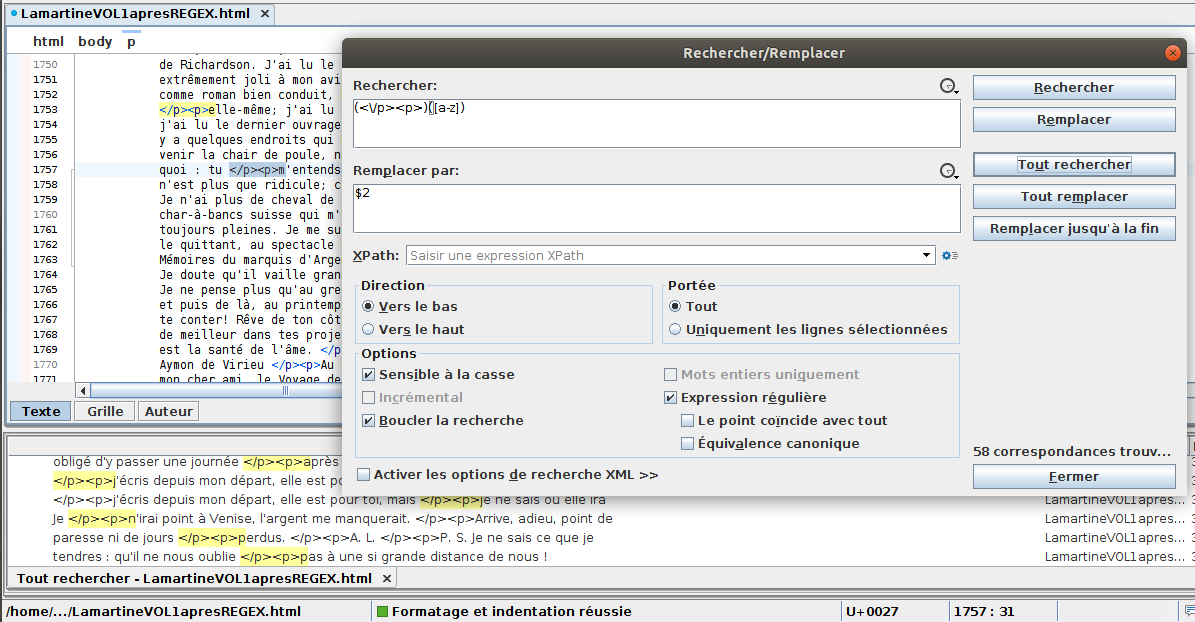
\includegraphics[width=16cm]{images/regex_p.png}
    \label{regex_p}
\end{figure}

Ici, nous matchons donc les deux balises \citecode{<p>} et nous mettons des parenthèses. Nous matchons celles qui se trouvent avant des minuscules (donc en milieu de phrase).
Pour la substitution, nous écrivons \citecode{\$2} comme cela les \citecode{<p>} sont supprimés et le \citecode{\$2} qui fait référence à la deuxième parenthèse garde le contenu et n’enlève pas la première lettre du mot en minuscules.

Ainsi, les expressions régulières permettent un gain de temps considérable dans le nettoyage de l'HTML.

\subsection{Quelle granularité dans la correction ?}

Cependant, celui-ci suscite des questionnements~: dans quel mesure faut-il corriger les fautes ? Quelle correction faire ? Une correction technique ou orthographique ? 

\subsubsection{Une correction orthographique ?}

Venant d'un parcours plus littéraire, il nous a été en effet très difficile de fermer les yeux sur certaines fautes, quitte à ce qu'elles soient corrigées par la suite. En effet, il nous a paru parfois plus judicieux de corriger en amont, c'est-à-dire dans l'HTML, certaines fautes orthographiques que nous avions remarquées, avant que celles-ci ne soient dispersées dans divers fichiers XML-TEI (en effet, la suite de la procédure est de diviser l'HTML en de multiples fichiers XML-TEI, un fichier par lettre)~: corriger les fautes en amont permettrait donc de pouvoir matcher les fautes dans un seul fichier HTML. Ainsi, nous nous sommes permis de faire quelques corrections orthographiques, dont nous donnons quelques exemples. 

Tout d'abord, un des problèmes de l’OCR est qu'il « recolle» un mot qui a été divisé par un tiret, lorsqu'il est en fin de ligne. 
Un problème se pose lorsque le mot en fin de ligne a un tiret parce que cela fait partie d’une expression, comme à la ligne 4026 de l'HTML de Lamartine où l’expression « écris-moi » a été assemblée en un mot « écrismoi\footnote{5 matches.} ». C'est donc une fausse interprétation de l'OCR qui ne fait pas la distinction entre un mot \inquote{recollé} avec raison ou non.Tombant dessus par hasard, nous avons donc corrigé ce genre d'erreurs. De même, l'OCR confond parfois les \inquote{l} et les \inquote{t}. Ainsi, quand nous sommes tombée sur ce genre d'erreurs, nous avons remplacé \inquote{Celte} par \inquote{Cette}\footnote{17 matches} ou \inquote{lu} par \inquote{tu}\footnote{70 matches, en faisant attention à ne pas corriger faussement certains \inquote{lu} qui sont justes (11 matches)}.

Ainsi, lorsque cela s'y prêtait, nous nous sommes permis de corriger certaines fautes qui s'imposaient à nous. Néanmoins, ce  n'était pas notre travail de les rechercher. Ce n'était pas notre objectif. Nous devions plutôt traquer les fautes techniques.

\subsubsection{Avant tout, une correction technique}

En effet, notre priorité était plutôt de corriger les balises comportant des problèmes, comme nous l'avons souligné plus haut (balises mal fermées, balises superflues, balises divisant des phrases en deux paragraphes). 

Parmi les fautes qui nous ont retenue figurait le manque de certaines balises pouvant poser problème par la suite pour l'extraction avec Python. En effet, cette extraction se base sur certains marqueurs. Si ceux-ci sont mélangés de temps en temps au reste du texte, les lettres ne sont pas bien extraites. Ainsi, pour ce qui est de la correspondance de Lamartine, il manquait des balises \citecode{<p>}  pour séparer la signature des chiffres romains désignant une nouvelle lettre~: \citecode{<p>ALPH. DE LAM. LXII</p>}. Nous les avons donc ajoutées avec une regex, pour les soixante-cinq occurences~: \citecode{<p>ALPH. DE LAM.</p><p>LXII</p>} 

En effet, il s'agit avant tout d'assurer une bonne extraction avec Python du fichier HTML pour qu'il soit transformé en fichiers XML. Pour cela, la dernière phase de pré-traitement est de repérer les marqueurs du texte en vue de l'extraction.


\subsection{Premiers repérages des marqueurs}

Les marqueurs avaient déjà été signalés dans le cahier de charges~: à chaque édition imprimée correspondent des caractéristiques différentes. Ainsi, pour la correspondance de Lamartine, on remarque que les lettres sont séparées les unes des autres par un chiffre romain. Celui-ci manquait parfois, nous nous sommes donc permis de l'ajouter manuellement, comme pour la deuxième lettre de Lamartine. Pour Lamennais, les lettres sont délimitées par des chiffres arabes cette fois. Ceux-ci posent problème car ils ne sont pas bien reconnus par l'OCR. Par conséquent, ils ne peuvent pas être extraits facilement avec des regex dans Python puisqu'ils comportent des erreurs~: le chiffre 5 est souvent pris pour un \inquote{a}, le 5 et le 3 sont souvent confondus, et le 8 est pris pour un \inquote{S}. Au lieu de 15, on lit \citecode{l.'l}, au lieu de 19, on lit \citecode{I!\&gt;}, à la place de 44, on trouve \citecode{t4}, et \citecode{ftj} pour 63, \citecode{tH} pour 64, pour n'en citer que quelques-uns. Nous avons donc dû retravailler ces marqueurs pour assurer une bonne extraction des lettres. Enfin, les lettres de Proudhon n'avaient pas de délimiteur. Nous nous sommes donc servie de sa signature \inquote{P.-J. PROUDHON.} pour extraire les lettres.

\begin{figure}[ht]
    \centering
    \caption{Cahier des charges ELICOM, repérage des marqueurs de Lamennais}
    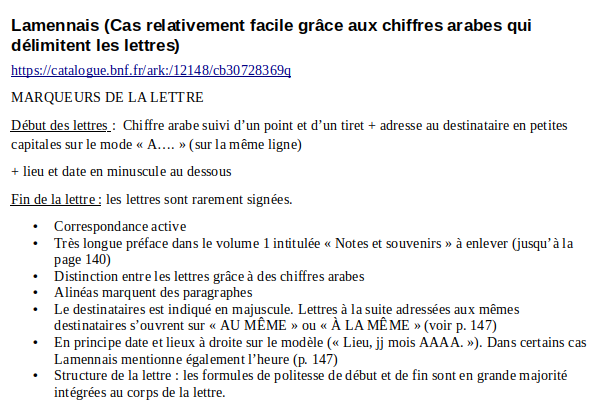
\includegraphics[width=16cm]{images/cdc_lamennais.png}
    \label{cdc_lamennais}
\end{figure}

Ainsi, l'OCR de Gallica s'est avéré être assez performant dans l'ensemble et nous a rendu de précieux services pour l'extraction de la correspondance en HTML. Bien-sûr, il reste quelques fautes à corriger, aussi bien au niveau de la structure de l'HTML qu'au niveau purement orthographique. Par ailleurs, nous n'avons pas encore évoqué la question de la mise en page qui n'est pas traitée par l'OCR, ce qui nous pénalise également. Nous y reviendrons lorsque nous parlerons des fichiers XML en quatrième partie. Néanmoins, le bilan est très positif pour l'OCR de Gallica. L'apprentissage machine a donc bien été au c\oe ur de l'acquisition des données pour notre projet d'ELICOM avec le Labex OBVIL. Il en est de même pour notre projet d'édition numérique de correspondance de Frédéric Le Play, même s'il se présente cette fois-ci sous la forme de l'HTR avec Transkribus.

\chapter{L'HTR de Transkribus}


\section{Quelle procédure pour l'acquisition des données ?}

\subsection{Rappels et point sur le corpus}

Il s'agit désormais d'acquérir les données pour notre projet d'édition numérique de la correspondance de Frédéric Le Play avec le CRHXIX. Avant tout, faisons un point sur le corpus en notre possession. Nous pensons pour l'instant éditer les  2091 lettres échangées entre Frédéric Le Play et 94 correspondants entre 1837 et 1882. 

En vue de leur mise en ligne, plusieurs étapes sont à suivre. Tout d’abord,avons-nous toutes les numérisations en notre possession, leur qualité est-elle suffisante ? De plus, les transcriptions ont-elles été réalisées ? Sinon, quelle procédure suivre pour réaliser ce travail ?

\subsection{S'assurer des numérisations des manuscrits}

Comme souligné plus haut, un travail de numérisation a déjà été engagé, et un récapitulatif a été fait sur les fonds numérisés\footnote{Voir fig. 3.1}. Il est en effet capital d'avoir une vue claire là-dessus car elles constituent la matière première, la base de notre travail. 

Plusieurs questions se posent sur la qualité de ces numérisations. En effet, comme nous l'avions déjà souligné dans notre deuxième partie\footnote{Voir 5.1.2},
\begin{quote}
    \inquote{Dans  le  cas  de la  publication  de  textes  en fac-similés [...],la  lisibilité  des  images  est  essentielle,  ce  qui  suppose  à  la  fois  une  attention  aux formats d’acquisition (qualité de l’image exprimée en dpi), et une juste évaluation des besoins de stockage et d’infrastructure matérielle pour la diffusion/communication de celles-ci\footnote{Ioana Galleron, Marie-Luce Demonet, Cécile Meynard, Idmhand Fatiha, Elena Pierazzo, etal., \emph{Les publications numériques de corpus d’auteurs - Guide de travail, grille d’analyse et recommandations}, 2018, URL~: \url{https://halshs.archives-ouvertes.fr/halshs-01932519/document}(visité le 05/05/2020).}}
\end{quote}
Or, si nombre de numérisations sont satisfaisantes car elles ont été commandées à des services d'archives ou bibliothèques, pour d'autres manuscrits, nous ne possédons que des photographies prises par des particuliers et qui sont floues ou d'une qualité médiocre, tant pour la précision que pour la prise de vue. Il s'agira donc de les faire numériser par des professionnels.

Par ailleurs, nous nous posons encore la question du format de l'image. Serait-il bon d'unifier les formats ? Nous avons tantôt des fac-similés en JPEG, tantôt des PDF ou encore TIFF (\emph{Tagged Image File Format}), plus rarement des PGN (\emph{Portable Network Graphics}). Il serait bon d'unifier les formats mais nous ne pensons pas que cela soit indispensable\footnote{Le retour en arrière aurait un coût probablement trop important alors que non indispensable}. L'important surtout est d'obtenir un fichier par page. C'est là que nous avons rencontré des problèmes avec certains PDF trop lourds, notamment ceux de la BNF et de la BIF, car ils comprenaient un trop grand nombre de pages~: il faudrait donc diviser les fichiers pour qu'il y ait un seul fichier par page numérisée\footnote{Par page numérisée, et non par lettre qui comprend parfois plusieurs pages}, que l'on pourrait ensuite appeler dans le fichier XML-TEI comprenant la transcription correspondante.

En vue de l’édition numérique de correspondance, il serait bon de privilégier les numérisations en couleur pour le design du site. La majorité, si ce n’est l’intégralité des sites d’édition numérique de correspondance possèdent des numérisations en couleur. Le but de mettre en ligne le manuscrit est de coller au plus près de la réalité matérielle.Dans ce but, la numérisation en couleur est préférable. Certes, nous possédons, notamment pour les fonds Peruzzi et Loyson, des numérisations en noir et blanc, qui sont d’ailleurs de très bonnes qualité. On pourrait à long terme songer à les remplacer par des numérisations en couleur, mais cela ne nous semble pas du tout prioritaire. Le site de Flaubert que nous avons déjà évoqué ne met pas toujours en ligne des fac-similés en regard, et certains sont en couleur, d'autres en noir et blanc. Certes, ce n'est pas parfait mais cela n'enlève rien à la qualité du site.

Par ailleurs, il faudra être attentif au nommage de chaque fichier, procédant toujours de la même manière, comme par exemple \citecode{expediteur\_destinataire\_fonds\_lettre1a.jpg}, en abrégeant les noms selon ce qui a été fixé. Ainsi, on pourrait écrire \citecode{lp\_ribbe\_arbaud\_l1b.jpg} ce qui signifie~: lettre de Frédéric Le Play à Charles de Ribbe, musée Arbaud, lettre 1, page 2 (pour le b)\footnote{Cette proposition reste encore un peu longue. On pourrait trouver quelque chose d'aussi précis mais de plus court.}.


Ainsi, avant tout, il s'agit de s'assurer de la bonne qualité des fac-similés et de leur bon nommage.
Ceci fait, on peut commencer à transcrire, puisque nous ne voulons pas seulement éditer les fac-similés. Nous voulons aussi avoir leur transcription en regard. Comment y parvenir pour ce corpus si important ? N'y aurait-il pas possibilité d'automatiser tout cela pour aller plus vite ?

\subsection{Transcriptions manuelles ou automatisées ?}
	
Nombre de manuscrits\footnote{Quelques centaines probablement, nous n'avons pas le chiffre exact.} ont déjà été transcrits manuellement, comme souligné plus haut, que cela soit par des étudiants, des doctorants, des stagiaires.
Or, la transcription s’avère être parfois un exercice difficile : les hommes du XIX\up{e} siècle disposent de certains codes d’écriture ou d’abréviations\footnote{Comme par exemple pour la date qui est souvent chiffrée différemment. Ainsi, ils écrivent 7bre pour septembre, Xbre pour décembre etc.} qui ne nous sont pas familiers. Par ailleurs, nombre de mots sont difficiles à lire, du fait des différentes écritures. Je pense par exemple à celle de Jules Baroche\footnote{Voir Annexe B.1 issue des premières pages du PDF SIM MS 6062 (p.7). Jules Baroche par exemple, lorsque deux « s » se suivent, allonge le premier. Ce sont les \inquote{s} longs que nous évoquions plus haut}.
Même avec un œil exercé, et des mains habituées à taper rapidement, il faut compter au moins cinq minutes par page pour la transcription, sans compter la relecture. En une heure, on peut donc transcrire douze pages, sans compter la relecture, ce qui nécessite deux-cents heures de transcription pour deux-mille lettres.

Ainsi, sur un corpus aussi important, comportant plus de deux-mille lettres, la question se pose d’automatiser les transcriptions en utilisant les moyens technologiques dont nous disposons aujourd’hui notamment avec l’apprentissage machine. C’est ainsi que nous avons fait le choix de nous tourner vers Transkribus.


\section{Transkribus, un outil de transcription}

\subsection{Transkribus, un pari}

Transkribus est un outil utilisé par de nombreux projets, mais il n’est pas forcément approprié à tous les corpus. Une transcription « manuelle » nécessite, certes, beaucoup de temps et une relecture attentive, mais entraîner une machine telle que Transkribus nécessite également beaucoup de temps, et ceci avec l’incertitude du résultat. 
S’il y a plus de 90 \% de taux de réussite, la transcription pourra se faire sans trop de difficultés, mais la relecture restera longue et nécessaire. S’il y a 98 \% de taux de réussite, c’est à nous de voir si nous acceptons ce taux d’erreurs ou si nous préférons relire pour un rendu plus optimal, mais également plus coûteux en temps, sachant que nous aurons de toutes façons les fac-similés en regard.

Par ailleurs, comme le soulignent les tutoriels mis en ligne pour initier à Transkribus, il faut \inquote{du temps pour explorer Transkribus et se familiariser avec son fonctionnement\footnote{Régis Schlagdenhauffen, \emph{Comment utiliser Transkribus en 10 étapes (voire moins)}, Site web de l'EHESS, URL~: \url{http://regis-schlagdenhauffen.eu/wp-content/uploads/2018/01/Comment-utiliser-Transkribus-\%E2\%80\%93-en-10-\%C3\%A9tapes-ou-moins.pdf} (visité le 22/05/2020).)}}. C’est donc un réel investissement au début, avec l’incertitude du résultat et la possibilité d’un échec.

Pour notre part, les résultats ont été dès le début encourageants. Sur 16 lettres, nous avons obtenu des scores de 84~\% d'erreur sur les caractères en entraînement. 
Nous avons donc continué cette aventure virtuelle, encouragés que nous étions par ces premiers retours.
Avant de présenter plus en détail notre travail sur Transkribus, il importe de présenter plus en détail cet outil.

\subsection{Un outil pensé par le READ}

\subsubsection{Le projet}

L' EADH, association européenne pour les humanités numériques (en anglais \emph{European association for digital humanities}), fondée en 1973\footnote{Sous le nom de \emph{Association for Literary and Linguistic Computing} (ALLC), voir \emph{About}, Site web de l'EADH, URL~: \url{https://eadh.org/about}, (visité le 23/09/2020).}, rassemble en son sein de nombreux projets pour faire avancer les humanités numériques\footnote{Le projet \emph{correspSearch} évoqué dans la deuxième partie en fait partie.}. Parmi eux, le projet READ\footnote{Projet lancé en 2015}, \emph{Recognition and Enrichment of Archival Documents} tient une place toute particulière. Comme son nom l'indique, il se consacre à la reconnaissance et à l'enrichissement des documents d'archives, visant à rendre les documents d'archives plus accessibles grâce à l'utilisation de technologies de pointe. L'objectif principal de READ est de fournir une plate-forme de services\footnote{Voir \emph{Accueil, Site web de Transkribus, URL~: }\url{http://transkribus.eu} (visité le 06/03/2020).} pour la reconnaissance, la transcription et la recherche automatisées de documents historiques. Entraîner les ordinateurs à lire du texte manuscrit de cette manière promet de révolutionner l'accès aux archives écrites. C'est dans cette optique que l'outil de transcription Transkribus a été conçu.

\subsubsection{L'outil}

Transkribus est un logiciel de transcription collaborative. 
Pour l'utiliser, il suffit de s'inscrire et de le télécharger. Puis, on peut importer les manuscrits en n'importe quelle langue, les transcrire manuellement, seul ou en équipe, en liant le texte à l'image grâce à la segmentation des images en régions de textes, lignes et mots réalisée à l'aide d'outils d'analyse de disposition. Puis avec ces transcriptions, on peut entraîner un modèle qui permettra à Transkribus de reconnaître par la suite l’écriture en question et d’effectuer lui-même les transcriptions.	

\subsection{Transkribus et l'apprentissage machine}

Transkribus s'utilise aussi bien pour l'OCR que pour l'HTR, mais ceux-ci diffèrent. En effet, 
\begin{quote}
    \inquote{La reconnaissance du texte manuscrit est un champ à part entière au sein des systèmes d’OCR. On parle d’ailleurs de \emph{Handwritten text recognition} (HTR) pour désigner le traitement des documents manuscrits, preuve qu’ils nécessitent des technologies spécifiques\footnote{\emph{in} Alix Chagué, \emph{ibidem.} p.42.}.}
\end{quote}
L'HTR n'est pas comme l'OCR, où, comme on a pu le remarquer avec l'OCR de Gallica, on appuie sur le bouton et le document est reconnu automatiquement. Qui dit HTR dit entraînement adapté à l'écriture d'une main particulière, sachant que cette main peut varier d'écriture ce qui rend l'entraînement d'autant plus fastidieux. Ainsi, Transkribus se doit d'entraîner des modèles\footnote{\emph{Handwritten Text Recognition Workflow}, Wiki de Transkribus, URL~: \url{https://transkribus.eu/wiki/index.php/Handwritten_Text_Recognition_Workflow} (visité le 23/09/2020).}. Pour cela, il est nécessaire de transcrire préalablement 100 pages, soit 15 000 à 20 000 caractères. 

En réalisant ce travail, nous participons de près ou de loin à l'objectif du READ. En effet, le but à long terme est d'entraîner le plus de styles d'écriture différents, de manière à ce que Transkribus soit en mesure de traiter la plupart des documents manuscrits sans entraînement préalable. Plus les utilisateurs travailleront avec Transkribus pour leur transcription, plus vite cet objectif ambitieux sera atteint\footnote{\emph{Questions and Answers}, Wiki de Transkribus, URL~: \url{https://transkribus.eu/wiki/index.php/Questions_and_Answers} (visité le 23/09/2020)..}. 

\subsection{Point sur la terminologie}

Avant de voir comment nous avons procédé avec Transkribus, il est utile de faire un point sur la terminologie en usage dans l'apprentissage machine\footnote{Voir \emph{ML | Introduction to Data in Machine Learning}, Site web GeeksforGeeks, URL~: \url{https://www.geeksforgeeks.org/ml-introduction-data-machine-learning/} (visité le 02/06/2020).. La figure 9.1 est tirée de cet article.}. Par ailleurs, l'anglais étant la norme en informatique, comment rendre les termes en français ? 

\begin{figure}[ht]
    \centering
    \caption{Les données dans l'apprentissage machine}
    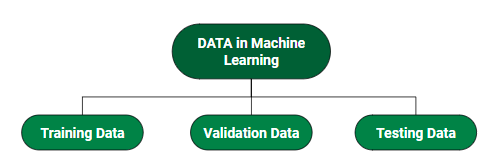
\includegraphics[width=16cm]{images/terminologieML.png}
    \label{terminologieML}
\end{figure}

Les données dans l'apprentissage machine se divisent en trois catégories, comme nous pouvons le voir sur la figure ci-dessus\footnote{Pour nous, les données en général sont les manuscrits. Mais en soi, les données peuvent être du texte, des sons et images etc.~: \inquote{\emph{It can be any unprocessed fact, value, text, sound or picture that is not being interpreted and analyzed}} \emph{In ibidem.}}~: 
\begin{itemize}
    \item Les données d'entraînement ou \emph{Training Data}~: ce sont les données que nous utilisons pour entraîner le modèle et qu'il apprend.
    
    Dans Transkribus, on appellera ces données \emph{Training Set}\footnote{Voir \emph{How to transcribe. Train a model}, Wiki de Transkribus, URL~: \url{https://transkribus.eu/wiki/images/3/34/HowToTranscribe_Train_A_Model.pdf} (visité le 23/09/2020), traduit en français~: \emph{Entraînement d’un modèle dans Transkribus}, Wiki de Transkribus, URL~: \url{https://transkribus.eu/wiki/images/8/84/Comment_entra\%C3\%AEner_un_Mod\%C3\%A8le_dans_Transkribus.pdf} (visité le 22/05/2020).} ou set d'entraînement\footnote{\emph{Entraînement d’un modèle dans Transkribus}, Wiki de Transkribus, URL~: \url{https://transkribus.eu/wiki/images/8/84/Comment_entra\%C3\%AEner_un_Mod\%C3\%A8le_dans_Transkribus.pdf} (visité le 22/05/2020).}. 
    
    \item Les données de validation ou \emph{Validation Data}~: elles sont utilisées pour évaluer le modèle d'après les données d'entraînement.
    
    \item Les données de test ou \emph{Testing Data}~: elles permettent d'évaluer la qualité du modèle une fois qu'il est entraîné. Le modèle prédit le taux d'erreur à chaque fois avec les données de test. D'une fois à l'autre, nous pouvons ainsi voir la progression du modèle par l'expérience. En effet, plus nous rentrons de données d'entraînement, plus le modèle acquiert de l'expérience, moins il se trompe, plus le taux de réussite est important et donc le taux d'erreur moindre.
    
    Pour Transkribus, pendant le processus de formation, quelques pages sont mises de côté à titre de test. Elles ne sont pas utilisées pour l'entraînement du modèle HTR+. Elles sont plutôt utilisées pour tester les performances de notre modèle\footnote{\emph{Idem.}, p.7}.
\end{itemize}

Ainsi, la plate-forme Transkribus permet aux utilisateurs d‘entraîner un modèle HTR+ de reconnaissance automatique de documents. Le modèle doit être entraîné pour reconnaître un style d'écriture particulier. Cela se fait en lui "montrant" les images et les transcriptions exactes correspondantes\footnote{\emph{Ibid.}, p.3}.

Voyons plus en détail comment procéder à l'acquisition des données pour notre projet avec l'outil de transcription Transkribus.

\section{Chargement des données d'entraînement et premier traitement}

\subsection{Procédure pour le chargement des données d'entraînement}

Pour charger les données d'entraînement, il y a toute une procédure à suivre. Il s'agit d'indiquer à la machine à quoi correspond tel caractère pour l'aider à apprendre l'écriture de Frédéric Le Play afin de pouvoir par la suite procéder elle-même aux transcriptions. 

Après avoir importé les données, on divise le texte en \emph{Text Region} (TR) ou régions de texte~: on lui indique où se trouve l'écriture. Puis on la lance pour que, dans ce cadre donné, elle tente de reconnaître elle-même où sont les lignes et surtout les \emph{base line} (BL), c'est-à-dire le trait à la base d'une ligne. En général, la Transkribus fait bien le travail, mais parfois, dès cette étape, on est en bute à certains dysfonctionnements lorsque la page comprend deux sens d'écriture.  

\begin{figure}[H]
    \caption{Résolution du problème de TR, deux sens d'écriture, capture d'écran de Transkribus}
    \centering
    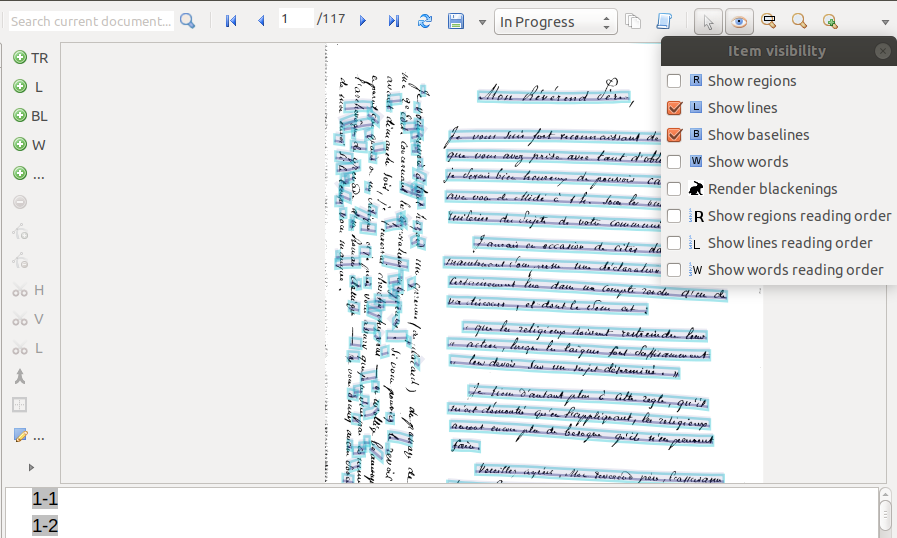
\includegraphics[width=7.5cm]{images/trTranskribus.png}
    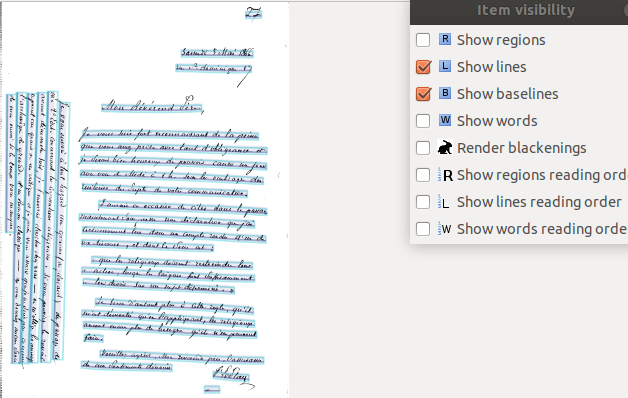
\includegraphics[width=7.5cm]{images/trCorrTranskribus.png}
\end{figure}

Transkribus se trompe alors totalement et reconnaît à la fois une multitude de lignes et de TR\footnote{Voir fig. 9.2}~: on peut gagner du temps en supprimant par TR (cela supprime du même coup les lignes que la TR a en son sein) mais quand il y a de multiples TR, on est obligé de tout supprimer à la main ce qui est une première perte de temps\footnote{Voir la version agrandie de ces deux images dans les annexes B.2}.\\

De même, quand Le Play utilise un papier légèrement strié pour écrire, celui-ci est confondu avec les caractères et considéré comme des lignes d'écriture\footnote{Voir fig. 9.3}. Il signale donc des lignes qui n'en sont pas. Ici, le mieux est de supprimer la TR et de mettre les BL manuellement, de gauche à droite et non l'inverse, sinon, la ligne apparaît en-dessous de la BL.\\

\begin{figure}[ht]
    \centering
    \caption{Problème de TR à cause du papier, capture d'écran de Transkribus}
    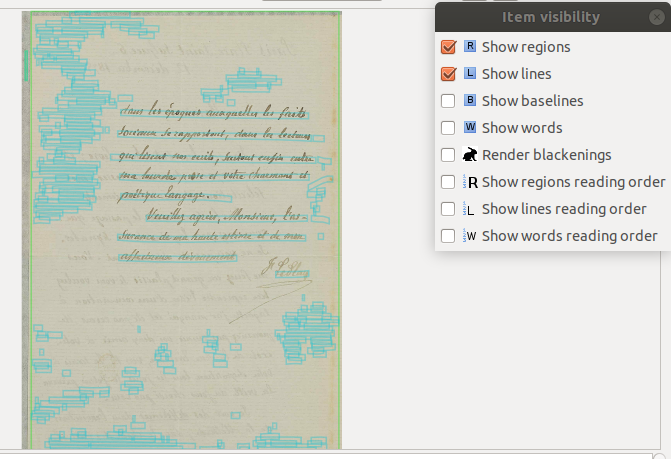
\includegraphics[width=13cm]{images/strieTranskribus.png}
    \label{strieTranskribus}
\end{figure}


Puis on peut procéder à la copie des transcriptions. Pour cela, on procède par copier/coller si les transcriptions ont déjà été réalisées, ce qui est notre cas. 
Néanmoins, cette phase nécessite une attention particulière. En effet, la mise en page et certaines graphies, lorsque l'on copie/colle, ne sont pas prises en compte. Il s'agit donc de les renseigner au fur et à mesure dans Transkribus. 

Transkribus permet ainsi d'indiquer les exposants, les mots qui ne sont pas clairs ou illisibles (\emph{unclear}), les mots barrés (\emph{strikethrough}), les mots soulignés(\emph{underlined}) etc.\footnote{Voir annexe B.3, fig. B.6, les styles de transcription en jaune.}..

Or, cette phase de chargement des données d'entraînement suscite d'autres questionnements sur les transcriptions. 


\subsection{Des transcriptions qui suscitent des questionnements}

\subsubsection{Des transcriptions de qualité variable}

Avant tout, nous avons commencé par importer les manuscrits dans Transkribus. Pour cela, il faut savoir lesquels nous désirons traiter en priorité. Notre choix s'est arrêté sur l'écriture qui ressort majoritairement du corpus en notre possession, à savoir celle de Frédéric Le Play. Ceci posé, nous avons commencé par importer dans Transkribus les manuscrits, puis les transcriptions qui avaient déjà été réalisées pour le CRHXIX. Nous avons dressé un tableau pour classer les correspondances à traiter en premier, en commençant par celles qui étaient de meilleure qualité quant à la numérisation et à la transcription, pour finir avec celles qui étaient de moindre qualité. En effet, certaines transcriptions ont déjà été relues ce qui est une garantie de meilleure qualité.

D'autres transcriptions faites par des étudiants n'ont pas encore été relues, par manque de temps, comportant des erreurs souvent dues à un manque compréhensible de familiarité avec les documents du XIX\up{e} siècle. Par ailleurs, certaines corrections notamment dans les accentuations ont été faites dans les transcriptions. Comment gérer ces différences par rapport aux originaux, alors que nous voulons justement charger des données pour apprendre à la machine à reconnaître les caractères ?

\subsubsection{Difficultés de transcriptions}

En une dizaine de jours, nous avons été amenée à rentrer 20 000 caractères dans le serveur de Transkribus afin d'entraîner le modèle pour l'écriture de Frédéric Le Play. 

De notre côté, nous n'avons pas fait de transcriptions à proprement parler, mais nous avons dû copier/coller les transcriptions réalisés par les étudiants et stagiaires pour le CRHXIX. Or, nous avons eu quelques doutes lors de la manipulation de ces transcriptions~: celles-ci n'étant pas toujours exemptes de fautes, nous nous sommes demandée dans quelle mesure nous devions les corriger.

Plusieurs questions émergent.

Tout d'abord, d'un point de vue purement technique, comment la machine peut-elle apprendre des caractères que nous-mêmes peinons à distinguer ? Ainsi, le \inquote{z} de Le Play est parfois écrasé et ressemble fort à un \inquote{r}~: cela a nécessité de notre part une certaine attention pour vérifier l'orthographe parfois incertaine des transcriptions d'une part, et d'autre part nous nous sommes demandée si la relecture des transcriptions opérées par Transkribus ne demanderait pas beaucoup de travail étant donné que les caractères sont souvent mal formés et donc difficiles à lire, et par l'\oe il humain, et par la machine, c'est du moins ce que nous craignons\footnote{Il est possible que par la suite, Transkribus sache mieux lire que l'homme, mais vu l'avancement du modèle de Le Play aujourd'hui, malgré les 20 000 caractères rentrés pour l'entraînement, ce n'est pas le cas.}. On constate ci-dessous que le \inquote{z} de \inquote{connaissez} pourrait être pris pour un \inquote{r}.

\begin{figure}[ht]
    \centering
    \caption{F. Le Play au R. P. Hyacinthe Loyson, 1866, capture d'écran de Transkribus}
    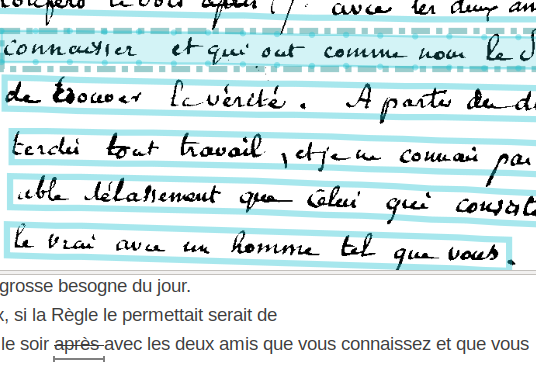
\includegraphics[width=12cm]{images/r-zTranskribus.png}
    \label{r-zTranskribus}
\end{figure}

Par ailleurs, nous avons dû être attentives à certaines mauvaises interprétations, comme par exemple, on lit dans la transcription~: \inquote{Que de bien à faire par le bon exemple ! car les sermons de vertu déposées [sic] pendant le moyen-âge ont percuté çà et là chez les vieillards. }

\begin{figure}[ht]
    \centering
    \caption{F. Le Play au R. P. Hyacinthe Loyson, 1866, capture d'écran de Transkribus}
    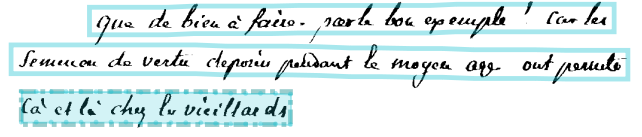
\includegraphics[width=16cm]{images/ma-Transkribus.png}
    \label{ma-Transkribus}
\end{figure}
Alors qu'il faudrait lire ce nous semble~: \inquote{Que de bien à faire par le bon exemple ! car les 
semences de vertu  déposées pendant le moyen âge ont persisté
çà et là chez les vieillards.}

Néanmoins, ces premières transcriptions même non relues sont d'une aide extrêmement précieuse~: le fait d’avoir déjà une grille de lecture aide à se mettre dans l’esprit du texte et à mieux saisir les possibles erreurs. C’est plus facile que si on aborde les textes avec un esprit totalement neuf. En outre, on peut bien dire qu'une des vertus de Transkribus est de nous permettre de réviser certaines transcriptions\footnote{À ce sujet, voir dans les livrables du CRHXIX le dossier \citecode{3-transcriptions} et l'explication dans les annexes.} 

On remarque ici par ailleurs la cédille manquante au mot \inquote{çà}, et l'accent circonflexe manquant sur le \inquote{a} de \inquote{âge} dans le manuscrit original. Par ailleurs, l'espace entre la préposition \inquote{par} et l'article défini \inquote{le} et si restreint qu'on croirait lire au premier regard \inquote{parle}. En trois lignes, on voit donc les complexités de transcriptions posées par l'écriture de Le Play.\\

Cette complexité se retrouve également face à certains mots difficilement lisibles et signalés comme illisibles par les premiers transcripteurs. Nous-même avons parfois peiné à saisir le sens de certains mots. Avec l'aide de l'équipe, nous avons pu venir à bout de certaines difficultés, comme ci-dessous\footnote{Fig. 9.6} où la graphie doublée des bavures de l'encre nous ont fait buter sur certains mots.  

\begin{figure}[ht]
    \centering
    \caption{F. Le Play au R. P. Hyacinthe Loyson, 1867, capture d'écran de Transkribus}
    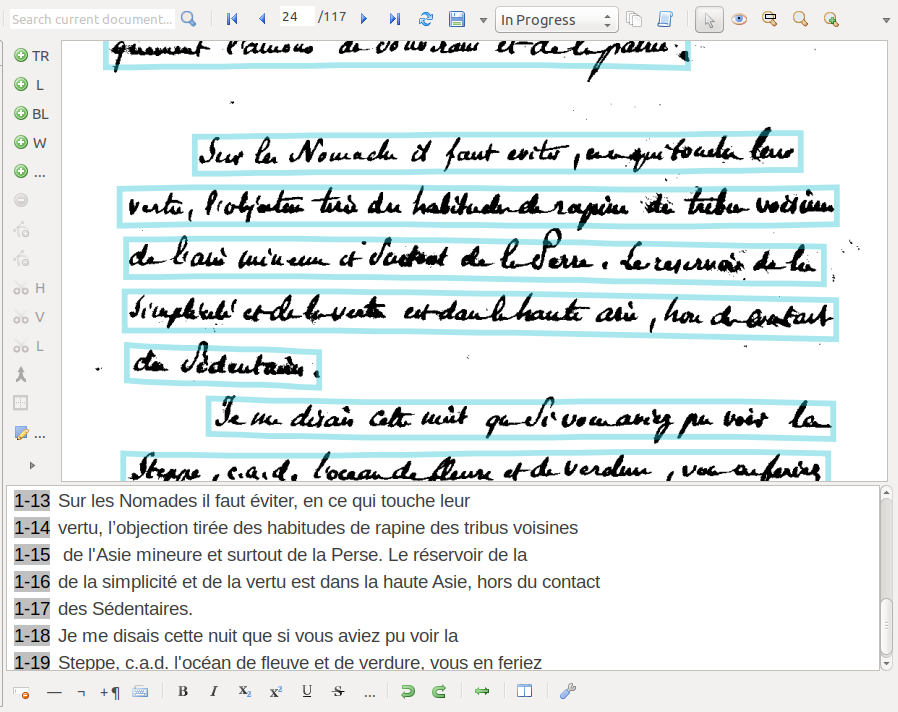
\includegraphics[width=16cm]{images/asieTranskribus.png}
    \label{asieTranskribus}
\end{figure}

\subsubsection{Transcriptions et principes de transcription}

Une des plus grandes difficultés pour nous a été aussi de faire la part des choses entre les majuscules justifiées ou non. Dans les principes de transcription évoqués plus haut\footnote{Voir 5.2.3.1}, il avait été convenu de respecter l’usage des majuscules par Le Play lorsqu’il semble avoir un sens précis, selon ses usages. Par exemple, Réforme plutôt que réforme ; ou les Autorités Sociales et de retenir l’usage
actuel lorsque les majuscules n’ont pas lieu d’être~: par exemple, \inquote{le concours de nos amis}, et non pas \inquote{le Concours de nos Amis}.
Cependant, certains cas particuliers nous ont laissée (peut-être à tort) perplexe. En effet, on remarque parfois une logique dans les majuscules chez Le Play. Faut-il la conserver ? Ici, Le Play écrit	\inquote{Vous remarquerez que dans mon Nouveau Plan, les anciens \underline{Chapitres}\footnote{Nous soulignons ici au lieu de mettre en italiques car nous reproduisons ce qui apparaîtra sur le site. Les mots soulignés et barrés apparaîtrons ainsi.}  deviennent des \underline{Livres} ; et que les anciens \underline{Paragraphes} deviennent des Chapitres.} 

\begin{figure}[ht]
    \centering
    \caption{F. Le Play au R. P. Hyacinthe Loyson, 1866, capture d'écran du manuscrit}
    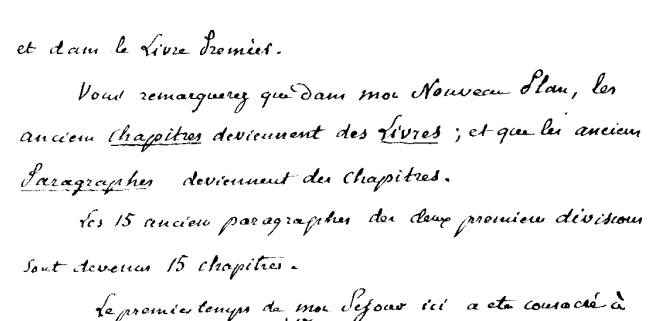
\includegraphics[width=16cm]{images/majusculesTranskribus.png}
    \label{majusculesTranskribus}
\end{figure}

En réalité, Le Play met des majuscules quand il veut insister sur un mot, qu'il souligne en plus de mettre une majuscule. Une fois que c’est établi, il continue sans majuscules :
\inquote{Les 15 anciens paragraphes des deux premières divisions sont devenus 15 chapitres}. Dans ce cas-là, pour notre part, nous serions pour conserver l'esprit de l'auteur de ces lettres en conservant la forme, et donc laisser les majuscules. Quant aux mots \inquote{Livre Premier} et \inquote{Nouveau Plan}, ils répondent également à la logique d'insistance de Le Play donc nous serions pour garder les majuscules. Néanmoins, nous enlèverions la majuscule à \inquote{Sejour} et ajouterions un accent aigu sur le \inquote{e} car c'est un autre cas de figure. La frontière est donc parfois difficile à voir entre la conservation ou non des majuscules.\\

\subsubsection{Des transcriptions qui ont pour but d'entraîner un modèle}

Une remarque s'impose~: nous rentrons ici des données d'entraînement en vue de la création d'un modèle qui permettra de transcrire automatiquement les lettres de Le Play. Si nous souhaitons que le modèle soit bien entraîné, il faut rentrer les données de façon brute, sans tri (majuscule ou non ? accent ou non ?). Ces questions ne devront se poser qu'au moment des relectures de transcription, après le travail de transcription sur Transkribus. Pour l'instant, nous devons respecter l'écriture de Le Play telle qu'elle apparaît sur le manuscrit, et non enlever des majuscules, ajouter des accents.\\

En revanche, c'est le moment où il s'agit de déchiffrer les mots classés illisibles par les premiers transcripteurs et corriger les fautes de transcription, ce que nous avons déjà évoqué plus haut.

Ici malheureusement, nous avons dû peu à peu lâcher du lest et baisser nos exigences. Comment pouvions-nous en si peu de temps coller entièrement au texte et corriger les premières transcriptions ? Rentrer 20 000 caractères n'est pas une mince affaire et représente une centaine de pages environ~: à la fin, nous avons été contrainte de nous contenter à faire des copiés/collés et corriger simplement les fautes qui sautaient aux yeux.\\

Une fois les caractères rentrés, il s'agit de procéder à l'entraînement du modèle, au fur et à mesure~: on peut constater ainsi la progression de l'apprentissage machine.

\section{Entraînement d'un modèle. Quels résultats ?}

\subsection{Mise en place de l'entraînement}

Peu à peu, on commence à entraîner le modèle. Plus on a de données d'entraînement, plus le modèle se perfectionne. 

On sélectionne les pages de transcription et on les met dans le \emph{Training Set}, puis on met de côté 10~\% des données dans le \emph{Validation Set} qui compare ce que nous avons transcris avec ce que la machine reconnaît après avoir été entraînée\footnote{Voir la figure 9.8 où on peut observer la sélection entre \emph{Training Set} et \emph{Validation Set}, juste avant de cliquer sur \inquote{OK} pour lancer l'entraînement du modèle. Ici, nous n'avions mis qu'une page pour le set de validation ce qui était normal car nous n'avions pas encore beaucoup de données et une page représentait donc environ 10~\%.}. 
\begin{figure}[ht]
    \centering
    \caption{Mise en place du premier entraînement du modèle Le Play}
    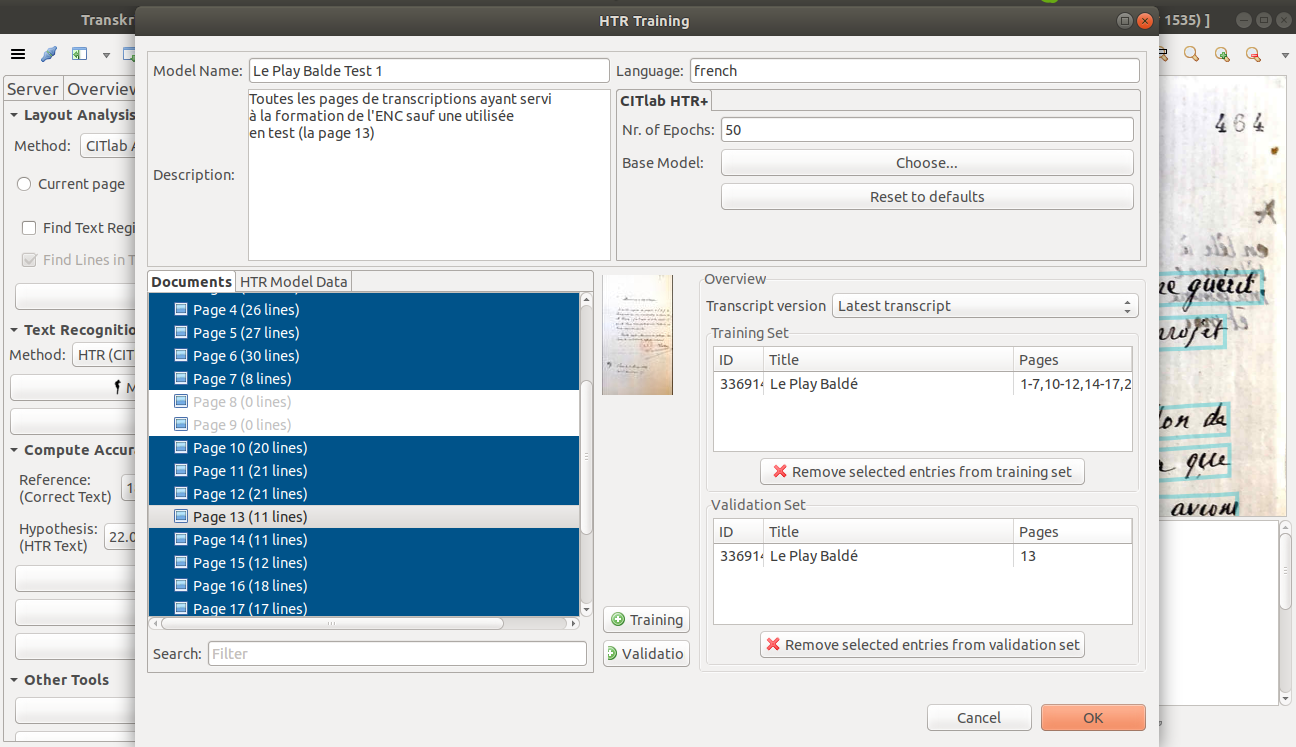
\includegraphics[width=16cm]{images/HTRtraining.png}
    \label{HTRtraining}
\end{figure}
Il est conseillé de prendre à chaque fois le même set de validation pour se faire une meilleure idée des progrès réalisés par l’apprentissage de la machine. De ce point de vue, notre entraînement du modèle a péché car nous n'avons pas mis assez de données de côté pour le set de validation. Nous pensions qu'il ne fallait mettre qu'une page alors qu'il fallait mettre 10~\%. Nous avons donc rectifié pour les derniers entraînements, mais cela fausse donc un peu la courbe de progression.\\

\subsection{Quelle progression du modèle, quels résultats ?}

Celle-ci est annoncée à la fin de chaque nouvel entraînement. On parle alors de \emph{Learning Curve} ou courbe d'apprentissage. On voit donc ci-dessous\footnote{Cf. Fig. 9.9} le graphique de la courbe d'apprentissage du premier entraînement du modèle Le Play. À gauche figurent tous les modèles disponibles, et tout en haut, en grisé, la ligne qui sélectionne le modèle qui nous intéresse et qui apparaît dans la colonne de droite.

\begin{figure}[ht]
    \centering
    \caption{\emph{Learning Curve} du premier entraînement du modèle Le Play}
    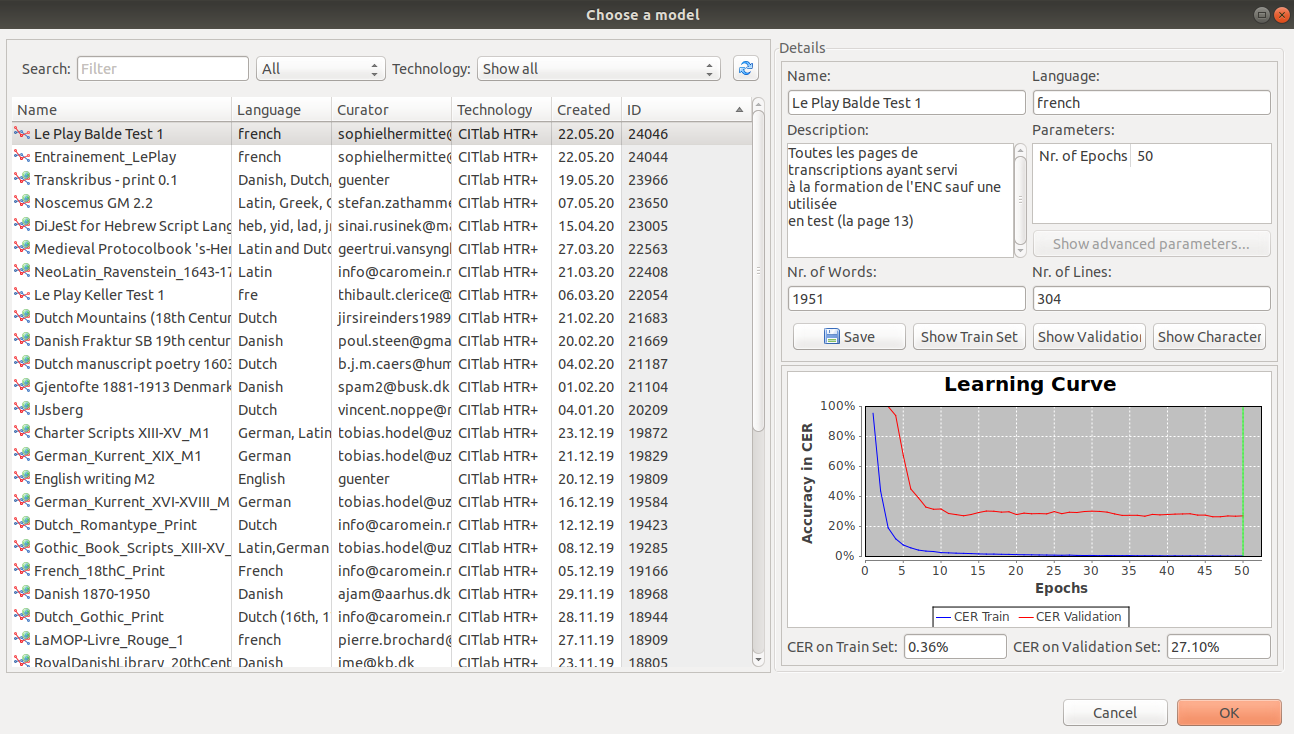
\includegraphics[width=16cm]{images/learningCurve.png}
    \label{learningCurve}
\end{figure}

Le taux d'erreurs de reconnaissance de caractères ou \emph{Character Error} (CER) définit l'efficacité du modèle. Cela représente le taux (en~\%) de caractères qui n'ont pas été
correctement transcrits par l‘HTR. L'idéal serait d'atteindre un CER inférieur à 5~\%, même si en soi un taux CER inférieur à 10~\% est déjà un taux satisfaisant.

Voyons plus en précision le graphique de la courbe d'apprentissage qui illustre la précision du dernier modèle entraîné\footnote{Cf. Fig. 9.10}, avec des données d'entraînement riches de 3146 lignes soit 23 729 mots.
 
 \begin{figure}[ht]
    \centering
    \caption{\emph{Learning Curve} du dernier entraînement du modèle Le Play}
    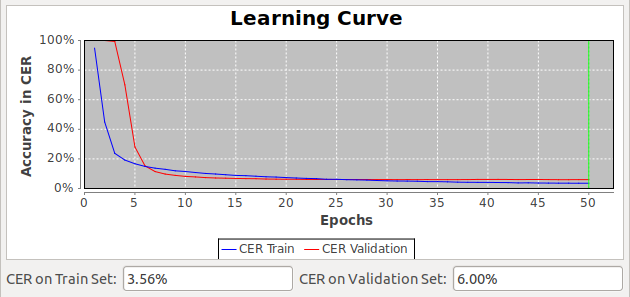
\includegraphics[width=16cm]{images/LearningCurveV4.png}
    \label{LearningCurveV4}
\end{figure}
 
Comme précisé dans le tutoriel fourni par Transkribus\footnote{\emph{Entraînement d’un modèle dans Transkribus}, Wiki de Transkribus, URL~: \url{https://transkribus.eu/wiki/images/8/84/Comment_entra\%C3\%AEner_un_Mod\%C3\%A8le_dans_Transkribus.pdf} (visité le 22/05/2020).}, l'axe Y définit l'\emph{Accuracy in CER} soit la précision en CER qui est affichée en pourcentage sur l'axe des ordonnées. La courbe
commence toujours à 100~\% et descend au fur et à mesure que l'entraînement progresse et que le modèle s'améliore.

L'axe X est défini comme \emph{Epochs} soit époques. Pendant le processus de formation, Transkribus effectue une évaluation après chaque époque. Lorsqu'on entraîne un modèle, on spécifie le nombre d'époques dans lesquelles le \emph{Training set} doit être divisé. Plus il y a d'époques, plus la formation dure longtemps. Ici nous en avons choisi 50.

Deux lignes apparaissent sur le graphique : une rouge qui indique l'état d'avancement des évaluations dans le jeu de tests et une bleue qui indique la progression de l'entraînement. \inquote{Le programme s'entraîne d'abord dans le \emph{Training Set}, puis se teste à l'aide des pages du \emph{Validation Set}.\footnote{\emph{Idem.} Tout ce qui est écrit ci-dessus s'appuie largement sur ce tutoriel.}}

\inquote{Au-dessous du graphique se trouvent deux pourcentages qui se réfèrent aux taux d’erreurs de l'ensemble d'apprentissage et de l'ensemble de test\footnote{\emph{Ibidem.}}}. Notre modèle a un taux d'erreur (CER) de 3,56~\% pour le \emph{Training Set}  et de 6~\% pour le \emph{Validation Set} sachant que nous avions rentré, comme le signale la figure 9.11, 23 729 mots pour le \emph{Train Set} et 1949 mots pour le \emph{Validation Set} (ce qui est insuffisant car cela représente un peu moins de 10~\%. Il manque environ 400 mots).

 \begin{figure}[ht]
    \centering
    \caption{Détails sur le jeu de données}
    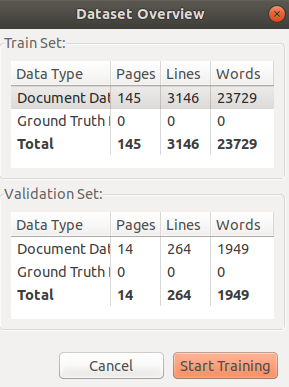
\includegraphics[width=5cm]{images/ToutLPV4datasetOverview.png}
    \label{ToutLPV4datasetOverview}
\end{figure}

La valeur de l'ensemble de validation est significative car elle montre comment le modèle se comporte sur les pages où il n'a pas été formé. Un taux de 6~\% est plutôt bon.\\

Si l'on récapitule la progression de l'entraînement du modèle, elle  s’est avérée être riche de promesses. 
\begin{itemize}
    \item Ainsi, en partant à 1849 mots, on obtenait :

CER ON TRAIN SET :~16,31 \%

CER ON VALIDATION SET : 26,25 \%
\item Puis, avec 1 951mots :

CER ON TRAIN SET~: 0,36 \%

CER ON VALIDATION SET : 27,10 \%

\item Avec 1 977 mots :

CER ON TRAIN SET : 0,29 \%

CER ON VALIDATION SET : 12,57 \%

\item Avec 4 207 mots :

CER ON TRAIN SET : 0,86 \%

CER ON VALIDATION SET : 11,55 \%

\item Avec 15 928 mots :

CER ON TRAIN SET~:~2,58 \%

CER ON VALIDATION SET : 6,40 \%

\item Avec 18 531 mots :

CER ON TRAIN SET : 2,91 \%

CER ON VALIDATION SET : 7,83 \% (même set de validation que le précédent)

\item Avec 23 729 mots :

CER ON TRAIN SET~:~3,52 \%

CER ON VALIDATION SET : 6,09 \% (même set de validation que le précédent)

\end{itemize}

Cependant, certains de ces chiffres sont biaisés car nous n'avons pas toujours utilisé le même set de validation, excepté pour les trois derniers entraînements du modèle. 

Par ailleurs, certains chiffres peuvent laisser dubitatifs car ils sont fluctuants. Cela est probablement dû à la part d’aléatoire du \emph{machine learning} en entraînement et peut-être aussi à cause de certaines images d'une qualité insuffisante.

Nous étions plutôt confiants quant aux chiffres indiquant la progression du modèle. 
En effet, si on traduit le CER en taux de réussite, nous sommes près d'un taux de réussite de 95~\% ce qui est très positif. 

Néanmoins, 5 \% de CER signifie tout de même une faute tous les 20 caractères, soit, pour une moyenne de 4 lettres par mot, 1 faute tous les 5 mots au moins.

Ceci étant établi, il est temps de voir si la réalité que cachent ces chiffres sera aussi positive qu'on l'espère : il s'agit désormais d'appliquer le dernier modèle pour que la machine opère elle-même les transcriptions. C'est l'aboutissement de notre travail. 
 
 
\section{Application du modèle}

Ayant trouvé la progression de l’entraînement du modèle plutôt bonne quant aux chiffres, nous étions assez confiante pour l’appliquer sur des manuscrits non transcrits et voir le résultat du travail d’une petite dizaine de jours.

Nous avons donc, à cette fin, mis de côté des manuscrits venant de fonds divers et variés représentant huit pages.

Pour appliquer un modèle et donc effectuer une transcription sur un manuscrit, il faut auparavant importer les manuscrits en question sur Transkribus. Puis, il faut se rendre dans l'onglet \emph{Tools} où se trouvent les outils, aller dans la partie \emph{Text recognition} et cliquer sur \inquote{Run}. Une fenêtre s'ouvre alors et l'on peut choisir les modalités de transcription et sélectionner le modèle dont on se sert pour transcrire : à chaque écriture correspond en effet un modèle adapté. Pour notre part, ayant entraîné un modèle pour l'écriture de Le Play uniquement, en toute logique, nous n'avons chargé que des manuscrits ne comportant que l'écriture de Frédéric Le Play.

Ceci fait, nous sommes allée regarder quels étaient les résultats des transcriptions automatiques. Or, pour la première page, il n'y a pas un mot sans faute, à part le « Monsieur » et la signature de Le Play. Nous avons pensé que cela était peut-être dû à la mauvaise qualité de la numérisation d'une part, et d'autre part peut-être du fait que nous n'avions entraîné pour le modèle aucune lettre de ce fonds\footnote{La première page transcrite automatiquement provient des archives départementales (AD) de Haute-Savoie, c'est une lettre de Le Play à Joseph Despine.}.

Une page est tirée du fonds de Frédéric de Mercey à la BNF. La qualité de la numérisation est donc plutôt bonne. Cependant, même si le résultat est meilleur que la précédente lettre, il reste encore beaucoup de fautes, et nous nous sommes demandée si le fait de les corriger ne prendrait pas plus de temps que de tout transcrire en partant de rien. Là encore, nous n'avions pas transcrit de lettres de ce fonds pour l’entraînement. Par ailleurs, l’écriture de Le Play varie selon son âge, et nous n'avons peut-être pas fourni de données d'entraînement comprenant toutes les périodes de la vie de Le Play. En effet, ici, l'écriture est plus fine, plus penchée, plus jeune, ce qui a peut-être posé problème pour la reconnaissance.

Une page est tirée de la bibliothèque publique universitaire de Genève~: c’est une lettre de Frédéric Le Play au père Hyacinthe Loyson. Nous avons entraîné près de 90 pages de ce fonds. Nous avons trouvé malgré cela bon nombre de fautes. D’autre part, la numérisation comportant des nuances de gris assez foncées, la machine l’a pris pour de l’écriture : cela demandera beaucoup de temps de corriger ces fautes car la machine matche à chaque fois une ligne qui n’en est pas une et croit y reconnaître de l’écriture. Il faut donc tout effacer et tout corriger.

 \begin{figure}[ht]
    \centering
    \caption{Lettre de F. Le Play au R. P. Loyson, 1870}
    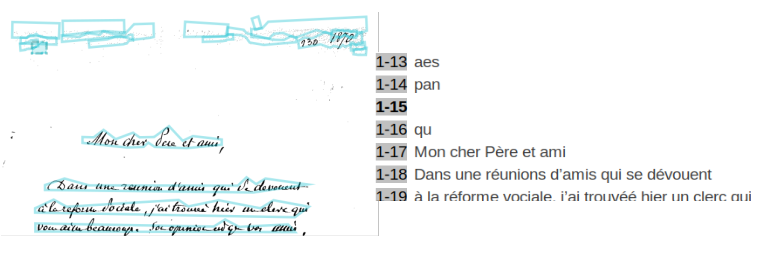
\includegraphics[width=16cm]{images/loyson.png}
    \label{loyson}
\end{figure}

Deux pages sont tirées du fonds conservé au Château de Ligoure, ce sont des lettres de Le Play à son fils Albert. La transcription est assez propre, mais subsistent encore bon nombre de fautes. Le Play forme parfois mal ses lettres, ce qui ne facilite pas la tâche, et pour l’œil humain, et pour la machine, comme nous l'avions déjà fait remarquer plus haut, ce qui d'ailleurs est aussi visible sur la figure 9.12. Par ailleurs, même si les mots sont reconnus, les accents sont souvent absents. (Par exemple, il est écrit senat pour sénat). Par ailleurs, Le Play a tendance à gommer les différences entre les majuscules et les minuscules. Souvent, ses « s » minuscules semblent être des « s » majuscules. En revanche, le « A » de « Albert » pourrait être une  minuscule, d’où de nombreuses majuscules prises pour des minuscules. 

Pour une lettre de Le Play à Alfred Tylor, le résultat est plutôt satisfaisant. La machine bute face à certains obstacles : les ratures. 

 \begin{figure}[ht]
    \centering
    \caption{Lettre de F. Le Play à Keele}
    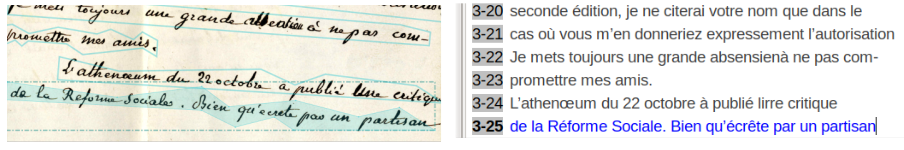
\includegraphics[width=16cm]{images/keele.png}
    \label{keele}
\end{figure}

Cependant, le résultat est plutôt bon dans l’ensemble, et la bonne qualité de la numérisation joue probablement un rôle dans ce sens. 

Pour une lettre de Le Play à Peruzzi\footnote{\emph{Biblioteca Nazionale Centrale} (Florence)
}, le résultat est plus que médiocre. Une des raisons de cet échec est la mauvaise délimitation des lignes : il y a deux sens d'écriture et la machine ne sait le reconnaître. Corriger ce genre d’erreurs prend plus de temps que de transcrire directement sans passer par la machine. Dans ce cas, il vaut mieux supprimer les lignes en question et transcrire soit-même. 

 \begin{figure}[ht]
    \centering
    \caption{Lettre de F. Le Play à Peruzzi, 1881}
    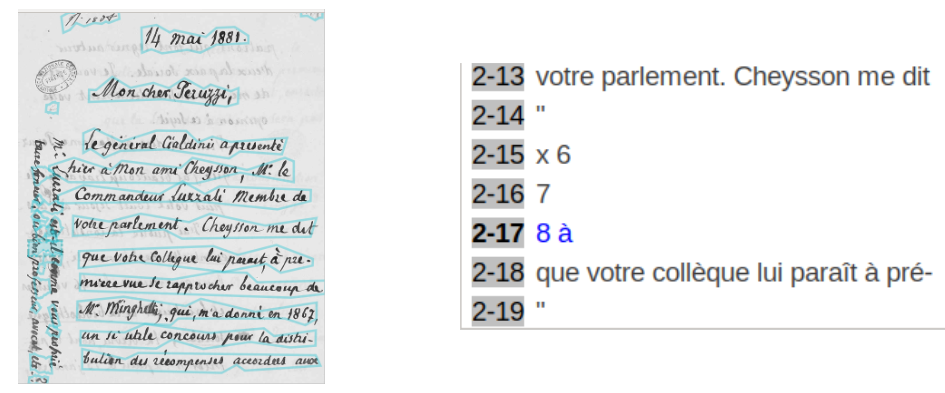
\includegraphics[width=16cm]{images/lpPeruzzi.png}
    \label{lpPeruzzi}
\end{figure}

Au terme de l'analyse de ces premières transcriptions réalisées avec notre modèle, nous avons été un peu surprise car nous pensions que les pourcentages annoncés promettaient moins de fautes.
 
Une question se pose : faut-il continuer à entraîner le modèle pour arriver à un résultat plus satisfaisant ou faut-il abandonner l’expérience ?

Deux possibilités s’ouvrent désormais : soit on entraîne encore le modèle, pour obtenir un meilleur taux de réussite, en faisant bien attention à prendre une écriture de Le Play qui couvre bien toute sa vie, car elle évolue avec le temps, (ce qui d’ailleurs nécessite d’avoir toutes les numérisations en main) et ceci avec le risque de n’avoir plus de lettres à transcrire une fois que l’on aura fini d’entraîner le modèle ; soit on laisse ainsi, mais il faudra effectuer une relecture et une correction qui risque de prendre presque autant de temps que la simple transcription : en effet, si l’on doit corriger une faute tous les cinq mots, le fait de rectifier quelque chose d’écrit pourrait prendre autant de temps que de bien transcrire directement et à la main. 

Quoi qu’il en soit, même si Transkribus n’est pas utilisé pour la transcription automatisée, avec le modèle, l’on peut toujours l’employer pour la transcription manuelle. En effet, Transkribus a le grand avantage de pouvoir être utilisé par plusieurs personnes du même projet à la fois. Ces dernières peuvent transcrire et leurs transcriptions resteront disponibles et ouvertes à toutes les personnes du groupe, ce qui permet de ne pas perdre les transcriptions dans l’ordinateur de l’un ou de l’autre. Par ailleurs, on peut ainsi mieux coller au texte, ayant le manuscrit visible sur la même page. On y trouve donc nombre d’avantages, même si l’on ne pousse pas la machine jusqu’au bout de ses capacités. Transkribus est un excellent outil de transcription collaborative qui permet d'avoir l'image et sa transcription en vis-à-vis ce qui est très confortable pour transcrire, même manuellement. 

Par ailleurs Le Play a une correspondance dont le nombre de lettres varie selon les correspondants, et si la majorité des lettres dont nous disposons sont écrites de sa main, beaucoup sont également des lettres passives. Certaines sont nombreuses, comme celles par exemple de Napoléon-Joseph Bonaparte\footnote{On dénombre 98 lettres de Napoléon-Joseph Bonaparte à Frédéric Le Play.}, mais d’autres sont rares, comme celles de Louis-Joseph Buffet\footnote{Louis-Joseph Buffet n’adresse que deux lettres à Le Play. }. 

Reste enfin la question de l’export des données, une fois que les transcriptions ont été réalisées, pour les encoder en vue de l’édition numérique de correspondance qui est tout l’objet de notre projet.


\section{Rester maître de ses données}

\subsection{Exportation en vue de l'édition}

Une fois que les transcriptions sont réalisées, il s'agit de les exporter. En effet, si elles sont toutes conservées dans le serveur de Transkribus, cela ne signifie pas que nous les avons dans nos serveurs propres. Il s'agit donc d'exporter les données pour les conserver au CRHXIX et rester maître des données : nous ne savons pas comment Transkribus va évoluer, si l'outil deviendra payant ou ne sera plus maintenu, il est donc important d'assurer ses données. 

Il faudrait penser également à la question du stockage des données, mais nous n'avons pas eu à la traiter durant notre stage, cela se fera par la suite. \\

Une question surtout se pose : comment exporter les données ? Plusieurs formats sont disponibles : \inquote{le package complet comprenant les fichiers image d'origine, les fichiers XML et les métadonnées ajoutés au document, un PDF (avec le texte transcrit inclus), doc et TEI. Tous les fichiers sont stockés dans un dossier\footnote{Régis Schlagdenhauffen, \emph{Comment utiliser Transkribus en 10 étapes (voire moins)}, Site web de l'EHESS, URL~: \url{http://regis-schlagdenhauffen.eu/wp-content/uploads/2018/01/Comment-utiliser-Transkribus-\%E2\%80\%93-en-10-\%C3\%A9tapes-ou-moins.pdf} (visité le 22/05/2020).)}}.

En vue de notre édition numérique de correspondance, nous avons exploré les différents formats d'exportation possibles. Les formats TXT et TEI s'avèrent être particulièrement intéressants. 
Lequel des deux privilégier ? 
Pour cela, il s'agit de considérer de plus près la question des \emph{tags} dans Transkribus.

\subsection{La question des \emph{tags}}

Dans Transkribus, on peut déjà caractériser certains mots grâce à des \emph{tags}. Nous avons pensé dans un premier temps utiliser les \emph{tags}\footnote{\inquote{Un tag (ou étiquette, marqueur, libellé) est un mot-clé (signifiant) ou terme associé ou assigné à de l'information [...], qui décrit une caractéristique de l'objet et permet un regroupement facile des informations contenant les mêmes mots-clés}. Voir \emph{Tag (métadonnée)}, Wikipédia, URL : \url{https://fr.wikipedia.org/wiki/Tag_(m\%C3\%A9tadonn\%C3\%A9e)} (visité le 26/09/2020).} de Transkribus, afin d'annoter en direct nos données. 

De nombreux \emph{tags} sont disponibles dans Transkribus\footnote{Voir les annexes, B.3 : Schématisation du modèle d'information de Transkribus.}. 
Nous nous sommes donc livrée à cette expérience et avons constaté que l'annotation des \emph{tags} dans Transkribus prenait beaucoup de temps. L'exemple de la figure 9.15 ci-dessous illustre les 21 \emph{tags} que nous avons mis pour une seule page de manuscrit.

 \begin{figure}[ht]
    \centering
    \caption{Pour une page, 21 \emph{tags}}
    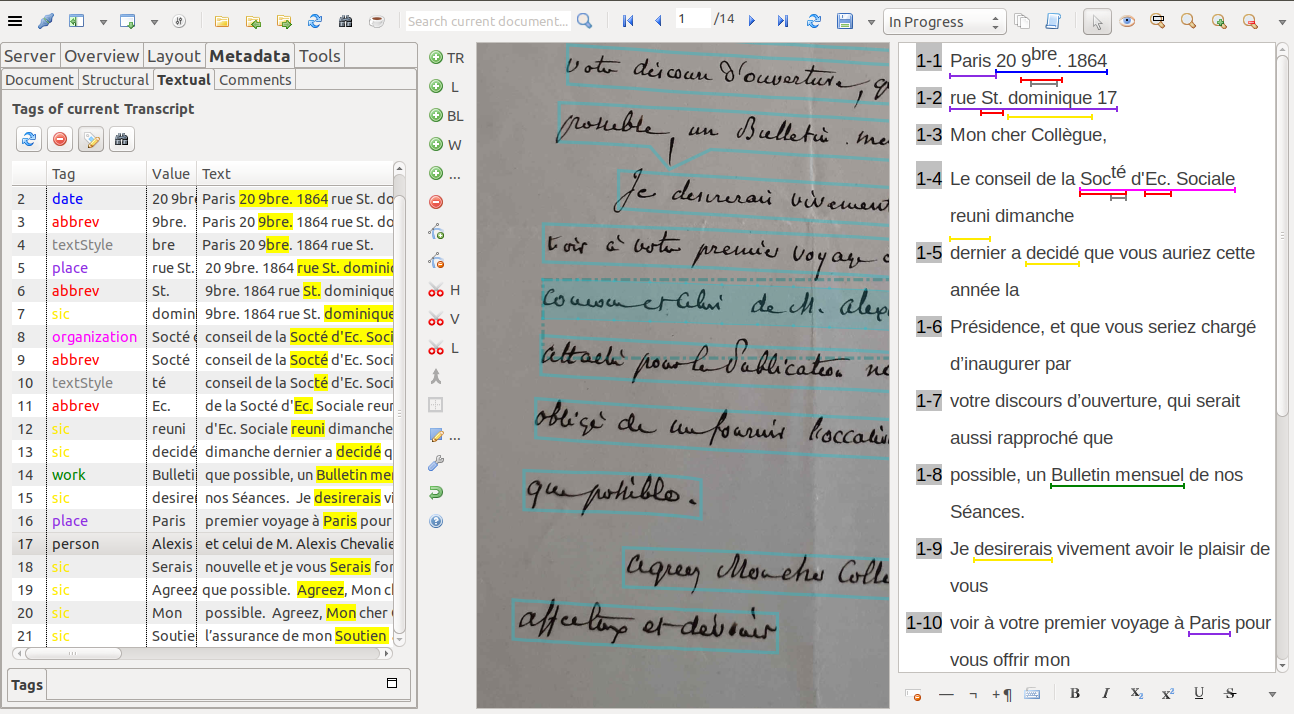
\includegraphics[width=16cm]{images/21tagTranskribus.png}
    \label{21tagTranskribus}
\end{figure}

En l'occurence, sur cette page, nous avons mentionné la date (\emph{date}), les abréviations (\emph{abbrev}), les exposants (\emph{textStyle)}), les noms de lieu (\emph{place}), les fautes dans l'original (\emph{sic}), les noms d'organisation (\emph{organization}), les noms d'ouvrage (\emph{work}), les noms de personne (\emph{person}).

L'avantage de renseigner en amont ces informations permet, lors de l'export, de les retrouver directement dans nos fichiers en XML-TEI. 
Cependant, nous n'avons pas opté pour ce choix pour plusieurs raisons : 
\begin{itemize}
    \item Nous avons été mise en garde sur l'export en TEI qui n'est pas encore tout à fait au point dans Transkribus
    \item Nous avons pris connaissance trop tard du guide d'utilisation des \emph{tags} dans Transkribus et de la possibilité de personnaliser ses propres \emph{tags}\footnote{\emph{How to enrich transcribed documents with mark-up}, \url{https://transkribus.eu/wiki/images/e/e8/How_to_enrich_transcribed_documents_with_mark-up.pdf} (visité le 26/09/2020).}.
    \item Nous aurions de toutes façons manqué de temps pour penser les \emph{tags} dans Transkribus à long terme
    \item L'export des \emph{tags} déjà existant s'est avéré être non conforme pour la TEI et nous avons dû corriger nombre de noms de balises.
    Nous aurions pu passer par une feuille de transformation (XSLT : \emph{eXtensible Stylesheet Language Transformations}) permettant de passer du fichier TEI exporté à un fichier TEI comportant les noms de balises que nous voulons mettre, mais ceci nécessite une bonne maîtrise de la technologie et nous pensons qu'il est préférable d'apprendre d'abord à l'équipe du CRHXIX à maîtriser XML au lieu de passer directement à la maîtrise d'XSLT. 
    \item Enfin et surtout, nous avons préféré penser le balisage directement dans XML-TEI. 
\end{itemize}

Quoi qu'il en soit, nous n'excluons pas pour le CRHXIX d'utiliser l'interface graphique de Transkribus pour les \emph{tags}. Il suffira à la personne qui prendra la suite de la partie numérique du projet de penser la chose. Nous avons de notre côté pensé surtout à l'enchaînement des balises.\\


L'export en TEI est tout de même intéressant pour ce qui est de la structure du texte (une balise délimite les lignes ce qui est intéressant). On peut également opter pour un export en TXT étant donné que la délimitation des lignes est également respectée. \\

Nous voyons que la phase d'acquisition des données s'est avérée riche en questionnements. L'apprentissage machine a eu une large part dans cette partie de nos stages, aussi bien pour l'OCR de Gallica que pour l'HTR de Transkribus. Que ce soit pour l'OCR ou l'HTR, nous n'en sommes pas encore à du 100~\% quant au résultat, néanmoins, ces technologies nous ont été d'un grand secours. La part de relecture reste tout de même importante. \\

Une fois les données acquises, il s'agit de les traiter en vue de leur valorisation et donc de leur mise en ligne. 
Qu'en est-il du traitement des données pour l'édition numérique de correspondance ? 
C'est l'objet de notre dernière partie.


\part{Traiter les données pour la réalisation des projets}

\chapter{Des standards et technologies au service de l'édition numérique}

Les données brutes, bien qu'intéressantes, ne nous permettent pas d'aller bien loin. Une fois que nous avons les transcriptions des correspondances à éditer, il s'agit donc de les traiter pour en assurer la mise en ligne, ce qui est tout l'objet de nos deux projets. Or, que ce soit pour le projet du CRHXIX d'édition numérique de la correspondance de Frédéric Le Play ou pour celui du Labex OBVIL, ELICOM, nous avons eu recours à XML, plus spécifiquement XML-TEI. Ce langage s'avère être en effet particulièrement adapté.

\section{XML, un langage particulièrement approprié}

Comme nous l'avions déjà souligné dans notre deuxième partie, lors de nos réflexions sur l'édition numérique de correspondance\footnote{Voir 4.1.2.3 XML}, XML est un langage structuré, à la fois lisible par l'\oe il humain et par la machine. 

\subsection{XML : présentation générale}
 
\subsubsection{Pourquoi encoder ?}
Le balisage sémantique permet d'expliciter certains aspects du texte\footnote{Voir aussi Elena Pierazzo, \emph{Why do we encode ?} URL : \url{https://www.youtube.com/watch?v=R0ncI_rr1z4&list=PL77mHK9JuenN9NXeXQbVcUORz7HZk-9Pv&index=2} (visité le 04/05/2020). Ce paragraphe s'en inspire.}. L'encodage est très utile pour l'édition car il permet de montrer la structure du texte, ce qu'il est, et non seulement son aspect, sa présentation. Il permet également de séparer le texte et le contenu de l'édition, et donc il permet différents modes d'affichage (notes, transcription normalisée ou non etc.).

Le balisage (\emph{markup}) et l'encodage (\emph{encoding}) n'ont pas été créés avec l'ordinateur, c'est un concept né avec l'imprimerie : en effet, les rédacteurs et éditeurs indiquaient par des symboles comment ils voulaient que le texte apparaisse, quelle taille de caractère, en gras ou en italiques par exemple. De même, la ponctuation et la mise en page sont aussi une sorte de balisage car elles permettent de comprendre comment diviser le texte en segments. Finalement, le balisage, c’est tout ce que nous utilisons pour rendre le texte plus lisible : l’espacement des lettres, les majuscules, le gras, l’italique, la ponctuation. Par ailleurs, encoder est un moyen de veiller à la pérennité des données, à leur conservation sur le long terme.

\subsubsection{Comment encoder ?}

Le langage XML est particulièrement approprié pour nos éditions numériques de correspondance. Il a été créé par le W3C en 1996, avec une contribution importante de la communauté des Humanités Numériques et en particulier de la TEI, comme nous l'avons déjà souligné plus haut.

\inquote{Les données sont incluses dans le document XML sous forme de chaînes de caractères délimitées par un balisage les décrivant. L’unité de base qui comprend données et balisage est appelée élément}\footnote{Voir Ariane Pinche, \emph{Séance 1}, Cours M2 TNAH XML, URL~: \url{https://github.com/ArianePinche/coursTNAH_XML-TEI/blob/master/seance01/InitiationXML.md} (visité le 09/10/2020).}.

Un élément est tout ce qui peut être étiqueté, tout ce qui se décrit, en quelque sorte, tout ce qui est important et devrait être annoté dans le texte.

L'élément a une balise d'ouverture qui se présente avec un chevron (\citecode{<)}), puis le nom du \emph{tag}, le contenu de l'élément puis la balise de fermeture qui a une barre oblique (\citecode{/)} : 

\citecode{<nomElement>chaineCaracteres</nomElement>}

Certains éléments peuvent être vides, dans ce cas on met une barre oblique à la fin : 

\citecode{<nomElement/>}

Les éléments suivent un ordre particulier : soit ils peuvent se suivre les uns après les autres, soit ils s'imbriquent, et dans ce cas, les éléments \emph{enfants} héritent des propriétés des éléments \emph{parents}. Jamais ils ne doivent se chevaucher.

Il faut aussi un élément qui contienne le fichier entier, on l'appelle \inquote{élément racine}.

Les éléments peuvent avoir des attributs, qui servent à préciser quelque chose de l'élément. L'attribut a une syntaxe particulière à respecter~:  après le nom de l’élément, il y a un espace blanc obligatoire, le nom de l'attribut suivi par un signe égal (\citecode{=}) et la valeur de l’attribut est entre guillemets. On peut avoir autant d’attributs qu’on veut dans l'élément mais le même attribut ne peut être utilisé qu’une seule fois\footnote{Pour aller plus loin, voir Ariane Pinche, \emph{ibidem} et les séances. suivantes}.

Un encodage qui respecte ces principes est dit bien formé. 

Par ailleurs, on peut distinguer trois types de balisages\footnote{Nicole Dufournaud, Valérie Gratsac Legendre. \emph{Manuel d’encodage XML-TEI - édition numérique de manuscrits baroques|: Recommandations pour une application TEI}, 2012, Site web HAL, URL~: \url{https://hal.archives-ouvertes.fr/hal-00718043/document} (visité le 28/07/2020).} : 
\begin{itemize}
    \item  Le balisage physique, formel et typographique encode les structures logique et formelle du texte
    \item  Le balisage sémantique autorise un encodage d'un premier niveau d'analyse comme les noms, les toponymes, les citations, les discours et les dates
    \item Le balisage analytique complète l'apparat savant de l'encodage.
\end{itemize}

\subsection{Les métadonnées}

Tout d'abord, pour bien gérer les données, il est important de les décrire au fur et à mesure. Ainsi, \inquote{préalablement à tout encodage, il est nécessaire de donner des informations descriptives et déclaratives sur le texte en vue de sa diffusion, d'un échange de données ou encore de son exploitation : ces composantes – ou métadonnées – forment l'en-tête TEI nommé \citecode{<teiHeader>}\footnote{Nicole Dufournaud, Valérie Gratsac Legendre, in \emph{Ibidem.}, p.7.}}

On entend par métadonnées 
\begin{quote}
    \inquote{les données servant à représenter ou   à décrire d'autres données, ici les deux textes édités. Elles contiennent des informations sur la source d'un document, sa nature, son contenu, sa localisation, son histoire, son statut juridique, etc. Elles remplissent un rôle d'indexation qui facilite l'accès au contenu et améliore la recherche. Elles doivent être normalisées grâce à des standards comme Dublin Core, EAD  (Encoded  Archival Description) par exemple afin de permettre l'interopérabilité et l'échange des données\footnote{\emph{Ibidem.}}.}
\end{quote}

Les métadonnées répondent donc à des standards. Or, la correspondance a ses standards propres : nous avons parlé plus haut du \citecode{<correspDesc>} pensé par le \emph{TEI SIG Correspondence}. Pour nos deux projets, nous avons suivi ces directives.

Par ailleurs, le projet ELICOM nous a éclairé dans le choix des métadonnées pour notre projet du CRHXIX, et nous retrouvons à peu près les mêmes informations, même si nous avons un peu plus détaillé le \citecode{<teiHeader>} pour le CRHXIX, avec notamment l'ajout de balises pour suivre les différentes mises à jour des fichiers XML-TEI.\\

Les métadonnées se trouvent donc dans le \citecode{<teiHeader>} et se subdivisent en un certain nombre de balises.\\

\subsubsection{La description bibliographique du document avec le \citecode{<fileDesc>}}
Tout d'abord, le \citecode{<fileDesc>} contient la description bibliographique du document. Pour ELICOM, il est réduit à deux éléments : \begin{itemize}
    \item le \citecode{<titleStmt>}\footnote{Pour le CRHXIX, nous avons ajouté quelques éléments à l'intérieur du \citecode{<titleStmt>} et du \citecode{<publicationStmt>}, le détail est indiqué dans l'ODD disponible dans les livrables, voir 1.4.2.1.1. Le titleStmt.} : il regroupe les informations sur le titre d’une œuvre et les personnes ou institutions responsables de son contenu intellectuel. C'est ici que sont nommés les principaux responsables du projet pour le CRHXIX. On indique les autres membres de l'équipe et ceux qui ont participé de près ou de loin au projet. Pour chaque personne, on utilise la balise \citecode{<respStmt> }qui englobe la balise \citecode{<resp>}, indiquant la responsabilité qu'a eue la personne en question, la balise \citecode{<name>} qui englobe le prénom puis le nom, et une balise \citecode{<note>} facultative, si jamais l'on a des remarques à faire. La balise \citecode{<note>} peut aussi comprendre un attribut \citecode{@resp} indiquant qui a rédigé la note.
    
    \item le \citecode{<publicationStmt>} : il informe sur la façon dont le projet est distribué ou publié. C'est donc ici qu'est renseignée la licence. Pour l'instant, nous n'avons pas encore déterminé pour le CRHXIX laquelle nous choisissons.
\end{itemize}


Pour le CRHXIX, étant donné que nous travaillons sur des fac-similés, nous y avons en plus ajouté le \citecode{<sourceDesc>}, élément capital pour l'édition numérique de correspondance. En effet, le \citecode{<sourceDesc>}, qui est une description de la source, contient le \citecode{<msDesc>} qui englobe les balises de description du manuscrit, à savoir la balise \citecode{<msIdentifier>} qui elle-même contient la balise \citecode{<country>}. Celle-ci indique le pays d'origine et peut comporter un attribut \citecode{@key} qui est facultatif. La balise \citecode{<settlement>} indique le lieu (ville ou autre), puis on renseigne l' \citecode{<institution>} qui abrite le manuscrit. La balise \citecode{<repository>} contient le nom d'un dépôt dans lequel des manuscrits sont entreposés, et qui peut faire partie d'une institution, et l'\citecode{<idno>} (identifiant) donne un numéro normalisé ou non qui peut être utilisé pour identifier une référence bibliographique.

Pour l'instant, nous ne voyons pas trop l'utilité de la balise \citecode{<msContents>} pour le projet du CRHXIX. Elle renseigne le contenu du manuscrit, décrivant le contenu intellectuel d'un manuscrit ou d'une partie d'un manuscrit, soit en une série de paragraphes \citecode{<p>}, soit sous la forme d'une série d'éléments structurés \citecode{<msItem>} concernant les items du manuscrit. Néanmoins, je laisse la possibilité de l'utiliser, mais on pourrait la supprimer par la suite.

En revanche, la balise \citecode{<physDesc>} pourra s'avérer utile. Elle contient la balise \citecode{<handDesc>} qui mentionne dans le \citecode{<handNote>} quelle main a écrit le manuscrit. Or, si Le Play écrit de sa main la plupart du temps, ce n'est pas toujours le cas, notamment quand il est malade. Pour les autres correspondants, le temps nous a manqué pour nous pencher sur la question, néanmoins, il sera toujours intéressant pour le lecteur non spécialiste et qui ne connaît donc pas les écritures, d'être informé du rédacteur du manuscrit.

\subsubsection{La description détaillée des aspects non bibliographiques avec le \citecode{<profileDesc>}}

Après la description bibliographique du document dans le \citecode{<fileDesc>}, on trouve une description détaillée des aspects non bibliographiques dans le \citecode{<profileDesc>}.

Un des éléments clés qui nous intéresse ici, et qui a été mentionné dans nos deux projets, est le \citecode{<correspDesc>}. Il comprend les informations de description de l'action liée à la correspondance. Celui-ci comprend principalement la balise \citecode{<correspAction>}. Celle-ci se décline en deux temps, selon ses attributs.

\begin{itemize}
    \item Tout d'abord, une balise \citecode{<correspAction>} avec un attribut type comprenant la valeur \citecode{sent} renseigne qui a envoyé la lettre. La balise \citecode{<persName>} comprend donc le prénom puis le nom de l'expéditeur (la plupart du temps il s'agit de Le Play). Elle comprend un attribut \citecode{@key} qui décrit l'expéditeur de façon normalisée et un attribut \citecode{@ref} qui renvoie vers sa fiche data.bnf. La balise \citecode{<settlement>} renseigne le lieu de rédaction de la lettre, et la balise \citecode{<date>} indique la date à laquelle la lettre a été écrite. L'attribut \citecode{@when} permet de la normaliser au format \citecode{AAAA-MM-JJ}. 
    
    \item Puis on retrouve une deuxième balise \citecode{<correspAction>} avec un attribut \citecode{@type} comprenant cette fois la valeur \citecode{received} renseignant à qui la lettre a été envoyée. La balise \citecode{<persName>} comprend donc le prénom puis le nom du destinataire. Elle comprend également un attribut \citecode{@key} qui décrit l'expéditeur de façon normalisée et un attribut \citecode{@ref} qui renvoie vers sa fiche data.bnf. Il y a possibilité d'ajouter une balise \citecode{<settlement>} renseignant le lieu de réception de la lettre, autrement dit le lieu où se trouve le destinataire, et la balise \citecode{<date>} indiquant la date de réception. L'attribut \citecode{@when} permet de la normaliser au format \citecode{AAAA-MM-JJ}. Cependant, il est bien clair que ces deux dernières informations ne seront quasiment jamais renseignées\footnote{Tout au moins c'est l'opinion que l'on peut avoir aujourd'hui, peut-être variera-t-elle dans le temps.}.
\end{itemize}
Ces choix du \citecode{<correspAction>} qui avaient été faits pour ELICOM nous ont donc inspiré pour le projet du CRHXIX.

Toujours dans le \citecode{<correspDesc>} l'on renseigne le \citecode{<correspContext>}, à savoir le contexte dans lequel se situe la lettre, quelle lettre la précède, quelle lettre la suit. On renseigne ces deux informations dans une balise \citecode{<ref>} avec un attribut \citecode{@type} de valeur \citecode{previous} pour la lettre précédente, de valeur \citecode{next} pour la suivante, et on le fait suivre d'un attribut \citecode{@target} qui fait pointer vers le fichier XML en question.

Dans le \citecode{<profileDesc>} se trouve également le \citecode{<settingDesc>} et le \citecode{<particDesc>}. Nous y reviendrons lorsque nous parlerons des index.

\subsubsection{L'historique du fichier avec le \citecode{<revisionDesc>}}
Le dernier élément du \citecode{<teiHeader>} est le \citecode{<revisionDesc>} qui résume l'historique des révisions pour un fichier.

Chaque changement est mentionné sous la balise \citecode{<change>}. Autrement dit, à chaque modification importante du fichier XML, on renseigne quelle modification a été faite (\citecode{<change>}), à quelle date avec l'attribut \citecode{@when}, par qui avec l'attribut \citecode{@who}.


\subsection{XML et le rituel épistolaire}

\subsubsection{Remise en contexte}
Avec XML, nous pourrions en soi encoder le monde entier, avec l'inconvénient sûr de s'y perdre. Il est donc important que le schéma de balise que nous serons amenée à choisir pour nos éditions numériques de correspondance soit le plus restreint possible. 

Par ailleurs, nous avons choisi de répondre aux conseils établis par la communauté scientifique et le TEI P5\footnote{Voir la partie 2 sur penser l'édition et \emph{TEI~: P5 Guideline}, TEI guidelines,  URL~:\url{https://tei-c.org/guidelines/p5/} (visité le 26/09/2020).}. Grâce aux \emph{TEI guidelines}, nous sommes face à des noms d'éléments définis. Il s'agit donc pour nous de suivre les directives du \emph{TEI : Correspondence SIG}. Il n'y a pas de place ici pour la fantaisie. Tout est bien normé. Il suffit simplement de définir quelles balises nous choisissons, et le cas échéant, dans quel ordre nous voulons qu'elles apparaissent.

Or, il faut que notre balisage rende compte des caractéristiques et de la structure propre à la correspondance. Comme nous l'avons vu plus haut, il y a ce qu'on appelle le \inquote{rituel épistolaire\footnote{ Richard Walter (dir.), \emph{L’édition numérique de correspondances – guide méthodologique}, URL :  \url{https://cahier.hypotheses.org/guide-correspondance} (visité le 17/06/2020). Voir particulièrement la page 13.}.}. Voici donc comment il peut se traduire  lorsqu'on encode : 

\begin{itemize}
    \item Le lieu de rédaction et la date apparaîtront en XML-TEI par la ligne \citecode{<dateline>} qui comprend les balises \citecode{<date>} pour la date et \citecode{<place>} pour le lieu
    \item Une \inquote{adresse} ou formule de politesse débutant la lettre, se traduira en balises par \citecode{<salute>}
    \item Une formule de politesse finale sera également transcrite dans un \citecode{<salute>}
    \item Une signature : en général, F. Le Play pour Frédéric Le Play. Si elle n'y est pas, on indiquera qu'elle est manquante, ceci dans la balise \citecode{<signed>}
    \item Éventuellement un post-scriptum qui trouvera sa place dans une balise \citecode{<postscript>}
\end{itemize}

Ainsi, la structure de la lettre est bien mise en évidence. L'encodage répond à nos attentes. Avant de développer le rituel épistolaire, remettons-le dans son contexte.\\

\subsubsection{Le \citecode{<body>}}
Cette structure de la lettre apparaît donc après les métadonnées du \citecode{<teiHeader>},dans la balise \citecode{<text>} qui comprend en général trois éléments : le \citecode{<front>} pour tous les éléments liminaires, le \citecode{<body>} pour le corps du texte proprement dit, le \citecode{<back>} pour tous les appendices, épilogues et postfaces. Pour nos éditions numériques de correspondance, nous développerons surtout la balise \citecode{<body>}.

Celle-ci comprend une division (\citecode{<div>}) avec un attribut \citecode{@type} dont la valeur est \citecode{lettre}. Si la lettre a été rédigée en deux fois, on peut donc utiliser plusieurs \citecode{<div>}, avec un attribut \citecode{@part} dont la valeur sera \citecode{I} pour le début ou partie initiale, \citecode{F} pour la partie finale, \citecode{M} pour le milieu si nécessaire. Cela permettra également d'ajouter une \citecode{<dateline>} pour les autres parties.

La première balise ensuite à mettre dans la \citecode{<div>} - uniquement pour l'édition numérique de la correspondance de Frédéric Le Play cette fois, car cela concerne les fac-similés - est la balise \citecode{<pb>}, qui permet de relier le fichier XML en question avec le manuscrit numérisé. On utilise tout d'abord un attribut \citecode{@n} pour renseigner le numéro du manuscrit, cela va de 1 à l'infini, et on peut y ajouter en plus une lettre en minuscule quand la lettre fait plusieurs pages et donc que le même fichier XML doit être mis en lien avec plusieurs images numérisées. Ainsi, la première page de la lettre 2 est numérotée 2a, la deuxième page 2b, la troisième page 2c et ainsi de suite.

L'attribut \citecode{@facs} pour les fac-similés pointe directement vers une image ou vers une partie d'une image correspondant au contenu de l'élément. On y met comme valeur le nom du fichier image, comme indiqué sur la figure 10.1.

\begin{figure}[ht]
    \centering
    \caption{Capture d'écran de l'ODD du CRHXIX, le \citecode{<pb>}}
    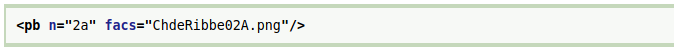
\includegraphics[width=16cm]{images/facs.png}
    \label{facs}
\end{figure}

Dès que l'on change de page de manuscrit au sein du même fichier XML donc de la même lettre, il faut donc à nouveau mettre la balise \citecode{<pb>} pour redonner toutes ces informations, entre la fin de la page précédente et le début de la nouvelle page.

\subsubsection{Le début de la lettre}
La balise \citecode{<opener>} souligne le rituel épistolaire. Elle abrite tous les éléments qui font débuter une lettre, à savoir l'élément \citecode{<dateline>} pour la ligne mentionnant le lieu (\citecode{<placeName>} avec attribut \citecode{@ref}, dont la valeur comprend un \citecode{\#}, pour pointer vers l'index) et la date (\citecode{<date>}) de rédaction de la lettre\footnote{Il faut encore décider si on normalise aussi à cet endroit la date avec un attribut \citecode{@when} ou si c'est inutile étant donné que cela a déjà été fait dans le \citecode{<correspDesc>} du \citecode{<teiHeader>}.}.

Le corps de la lettre nécessite parfois l'emploi d'autres balises pour traiter les cas particuliers\footnote{Encore une fois, ce paragraphe ne concerne que le CRHXIX, étant donné que nous avons affaire à des manuscrits qui n'ont jamais été publiés. La question ne se pose pas pour ELICOM qui travaille sur des éditions imprimées.}. C'est le cas des abréviations. Afin de garder les deux versions\footnote{La question n'a pas encore été tranchée pour le CRHXIX.}, la version originale et la version normalisée, on utilise une balise générale \citecode{<choice>} qui abrite deux balises : la première \citecode{<abbr>} garde l'abréviation originale de l'auteur. La deuxième \citecode{<expan>} donne le mot entier.

Une procédure assez similaire se fait pour la correction des fautes ou la normalisation des lettres. On utilise alors une balise \citecode{<choice>} qui englobe une balise \citecode{<sic>} qui contient le texte original, et une autre \citecode{<corr>} qui contient le texte corrigé.

 \begin{figure}[ht]
    \centering
    \caption{Capture d'écran de l'ODD du CRHXIX, l'\citecode{<opener>}}
    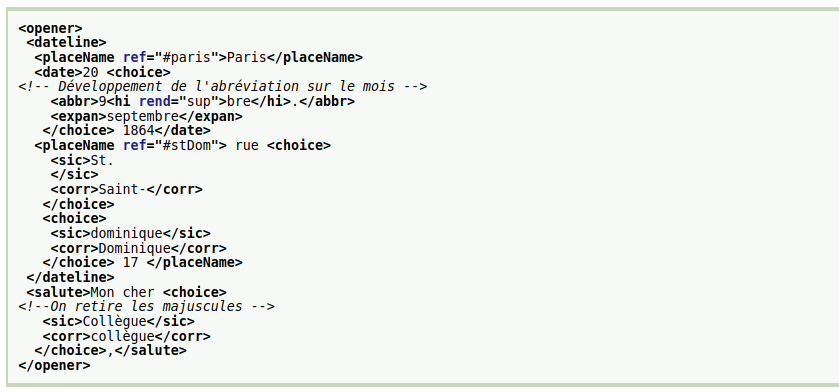
\includegraphics[width=16cm]{images/abbr.png}
    \label{abbr}
\end{figure}

A cela s'ajoute la question du style. Certaines lettres sont en italiques, soulignées etc. Pour manifester ces différents styles, on utilise la balise \citecode{<hi>} avec son attribut \citecode{@rend} qui spécifie la nature du style employé :
\begin{itemize}
    \item \citecode{"italic"} pour les italiques
    \item \citecode{"bold"} si c'est du gras
    \item \citecode{"upper"} pour la mise en capitales du texte sélectionné
    \item \citecode{"small-caps"} pour la mise en petites capitales
    \item \citecode{"sup"} pour la mise en exposant
    \item \citecode{"ul"} pour souligner
    \item \citecode{"line-through"} pour barrer.
\end{itemize}

La balise \citecode{<dateline>} renseignée, il s'agit ensuite de mettre dans la balise \citecode{<salute>} la salutation qui est faite au début de la lettre. Cela fait partie du rituel épistolaire.

Ceci fait, on passe au corps de la lettre.

\subsubsection{Le corps de la lettre}

Le corps de la lettre est contenu dans des balises \citecode{<p>}. Autrement dit, chaque paragraphe est contenu dans une balise \citecode{<p>}. Chaque ligne de ce paragraphe est contenu dans une balise \citecode{<l>}.

Il faut ensuite gérer les cas particuliers. Parfois, l'auteur de la lettre écrit lui-même des notes dans les marges\footnote{Tout ce qui fait référence à la mise en page dans nos dires ne concerne que le CRHXIX. Le reste concerne les deux projets, sauf avis contraire.}. Dans ce cas-là, on peut utiliser une balise \citecode{<note>}. On utilise un attribut \citecode{@resp} pour indiquer que la note a été rédigée par l'auteur de la lettre lui-même, et un attribut \citecode{@place} pour indiquer où la note se trouve dans l'original.

La valeur de l'attribut \citecode{@place} peut varier. Retenons quelques exemples :
\begin{itemize}
    \item \citecode{"above"} : au-dessus de la ligne
    \item \citecode{"below"} : au-dessous de la ligne
    \item \citecode{"bottom} : en bas de page
    \item \citecode{"inline"} : dans le corps du texte
    \item \citecode{"top"} : en haut de page
\end{itemize}

\begin{figure}[ht]
    \centering
    \caption{Capture d'écran de l'ODD du CRHXIX, l'attribut \citecode{@place}}
    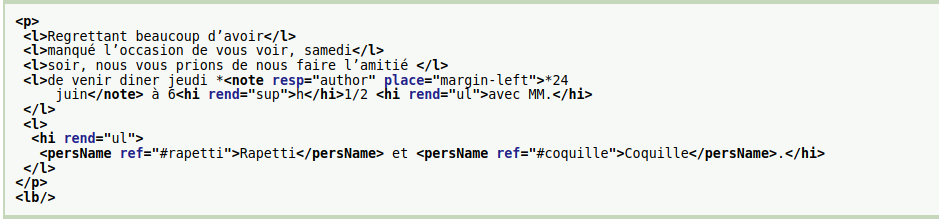
\includegraphics[width=16cm]{images/place.png}
    \label{place}
\end{figure}

Pour le corps de la lettre, nous avons été face à plusieurs questionnements pour ELICOM. En effet, les fichiers XML qui avaient été extraits de l'HTML\footnote{Nous reviendrons tout à l'heure sur cette extraction en parlant rapidement de Python.} comportaient des fautes d'OCR ou d'autres fautes de diverses nature. Par exemple, dans un fichier XML de la correspondance de Félicité de Lamennais, deux fautes sont visibles sur la même page\footnote{Voir Fig. 10.4} : on remarque d'une part un caractère \inquote{i} indiqué à la place d'une marque de crayon à papier. La faute d'interprétation de l'OCR est ici due à la qualité de la numérisation. Un livre usagé a été choisi pour la numérisation ce qui fausse le résultat de l'océrisation. D'autre part, on remarque un problème de guillemets à répétition. En effet, dans l'édition d'origine, les guillemets sont répétés à chaque ligne pour marquer que c'est une citation. Dans notre fichier XML, cela n'a plus de sens car ces guillemets polluent le corps du texte. Certaines modifications et corrections sont donc à apporter au fur et à mesure dans le corps du texte quand cela se présente.

\begin{figure}[ht]
    \centering
    \caption{Des fautes dans un fichier XML (154), Félicité de Lamennais, ELICOM. Capture d'écran d'Oxygen XML Editor et du PDF de l'édition originale.}
    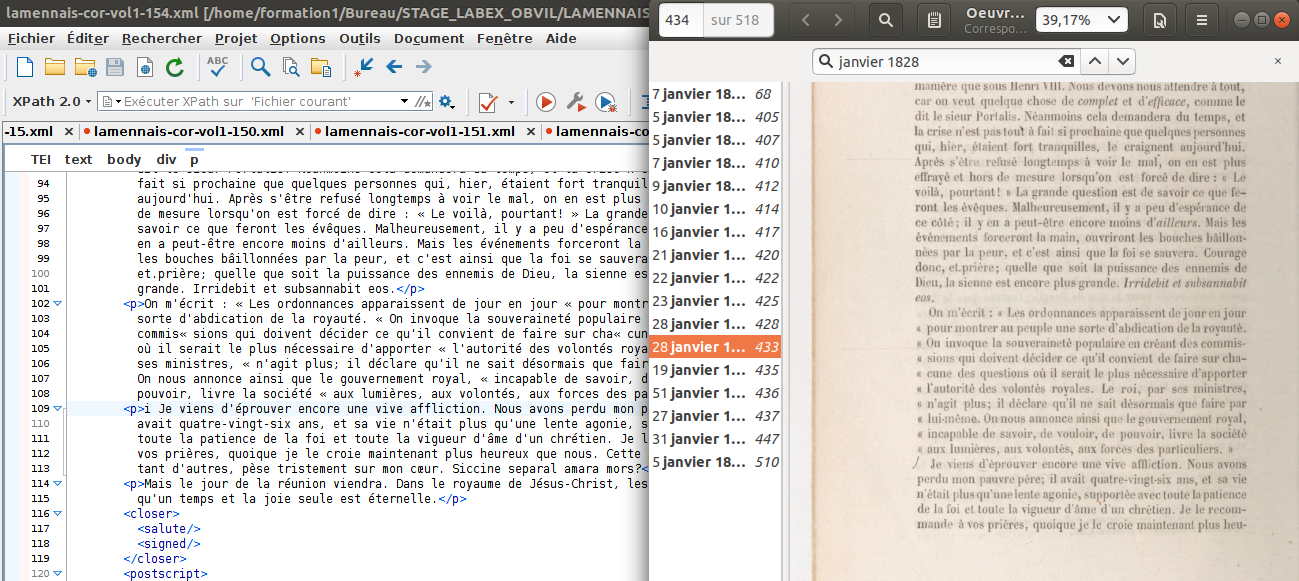
\includegraphics[width=15cm]{images/crayonPapier.png}
    \label{crayonPapier}
\end{figure}

De même, on remarque de faux paragraphes qui se forment ainsi à cause d'un changement de page et qui se doublent d'un tiret séparant le mot. L'ancienne mise en page de l'édition numérique apporte donc des erreurs dans le fichier XML. 

\begin{figure}[ht]
    \centering
    \caption{Faux paragraphes dans un fichier XML (159), Félicité de Lamennais, ELICOM. Capture d'écran d'Oxygen XML Editor et du PDF de l'édition originale.}
    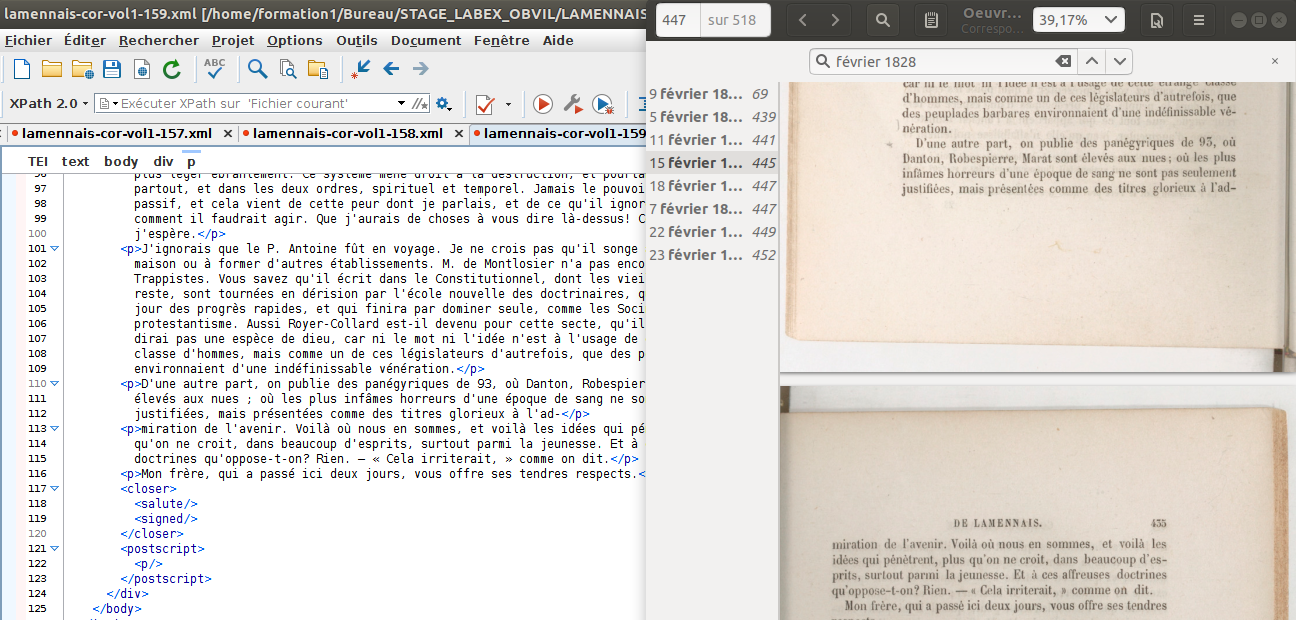
\includegraphics[width=15cm]{images/tirets.png}
    \label{tirets}
\end{figure}

Ainsi, la mise en place et relecture du corps de la lettre a dû être relativement attentive aux problèmes d'océrisation et autres fautes.

\subsubsection{La fin de la lettre}

La balise \citecode{<closer>} marque la fin d'une lettre et fait partie du rituel de correspondance.

Elle-même contient deux balises : d'une part \citecode{<salute>} qui comprend la formule de politesse concluant la lettre, d'autre part \citecode{<signed>} qui englobe la signature. Bien-sûr, la balise \citecode{<salute>} comprend des balises \citecode{<l>} encadrant chaque ligne, c'est toujours le même principe que dans le corps de la lettre. En revanche, les balises \citecode{<p>} ne sont pas admises dans la balise \citecode{<salute>}, probablement parce que les salutations ne font en général pas plus d'un petit paragraphe.

On peut mettre un attribut \citecode{@place} pour indiquer l'emplacement de la signature dans la lettre.

\subsubsection{Le post-scriptum}

La balise \citecode{<postscript>} contient l'éventuel post-scriptum. Elle contient des balises \citecode{<p>} et \citecode{<l>}.
C'est la dernière balise admise dans le corps du texte. Elle achève le fichier XML.

\subsection{Les index}

Par ailleurs, il s'agit de mettre en évidence dans le corps du texte les entités nommées déjà évoquées dans la deuxième partie de notre mémoire\footnote{5.1.2 Cinq dimensions à prendre en compte}. En effet, \inquote{on introduit un balisage dans un document pour l’étiqueter et l’organiser en vue d’un traitement automatisé. Si les paragraphes sont clairement marqués (balisés), alors un logiciel de mise en forme pourra les mettre en page correctement. Si les noms de lieu sont clairement marqués, un programme peut les sélectionner automatiquement pour générer un index géographique\footnote{Lou Burnanrd, \emph{Qu’est-ce que la Text Encoding Initiative~?}, Open Edition Press, 2015, URL~: \url{https://books.openedition.org/oep/1298?lang=fr} (visité le 26/09/2020).}}. Pour ELICOM, nous n'avons pas encore poussé très loin la granularité d'XML : nous avons commencé par transformer les fichiers HTML en fichiers XML sans aller encore très loin dans la description, particulièrement dans le balisage des entités nommées.
En revanche, dans le cadre de l'édition numérique de Le Play, nous nous sommes bien penchée sur la question\footnote{Cette partie sur les index ne concerne donc que le projet d'édition numérique de la correspondance de Frédéric Le PLay.}. Comme annoncé dans la deuxième partie, nous avons choisi d'élaborer six index : index des ouvrages cités, index des événements, index des noms de lieu, des noms de personne, des noms d'organisation, et enfin, index de vocabulaire leplaysien. 


D'une part, dans le corps du texte, à chaque mot indexé, il faut donner la possibilité de pointer vers l'index. Pour les noms de lieu on utilise la balise \citecode{<placeName>}.
\begin{figure}[ht]
    \centering
    \caption{Capture d'écran d'Oxygen XML Editor, pointer vers un index}
    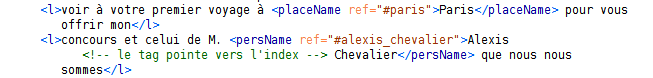
\includegraphics[width=16cm]{images/index.png}
    \label{index}
\end{figure}
Pour les noms de personne ou personnage, on utilise la balise \citecode{<persName>}. Pour les noms d'organisation on utilise la balise \citecode{<orgName>} et pour tous les autres index, on indique la balise \citecode{<name>}. Toutes ces balises ont un attribut \citecode{@ref} qui permet de pointer vers l'index en question avec un tag (\citecode{\#}).



D'autre part, les index en tant que tels se trouvent dans le \citecode{<teiHeader>}. 

\subsubsection{L'index des ouvrages cités}

Dans le \citecode{<sourceDesc>} se trouve un premier index, celui des ouvrages cités dans la correspondance. Tous se situent dans le même index, que ce soient des ouvrages écrits de la main de Le Play ou d'autres contemporains ou antérieurs. Nous avons choisi de renseigner aussi dans cet index les revues et les journaux. Pour les différencier des livres, nous avons pensé à ajouter un attribut \citecode{@type}, qui spécifie si c'est un journal ou une revue.

L'index des ouvrages est englobé dans une balise \citecode{<listBibl>}. Chaque ouvrage (livre, journal ou revue) est contenu dans une balise \citecode{<bibl>}, suivie d'une balise \citecode{<name>} pour le titre, \citecode{<author>} pour l'auteur, \citecode{<date>} normalisée avec l'attribut \citecode{@when}, et une balise \citecode{<note>} est facultative. \begin{figure}[ht]
    \centering
    \caption{Capture d'écran d'Oxygen XML Editor, l'index des ouvrages}
    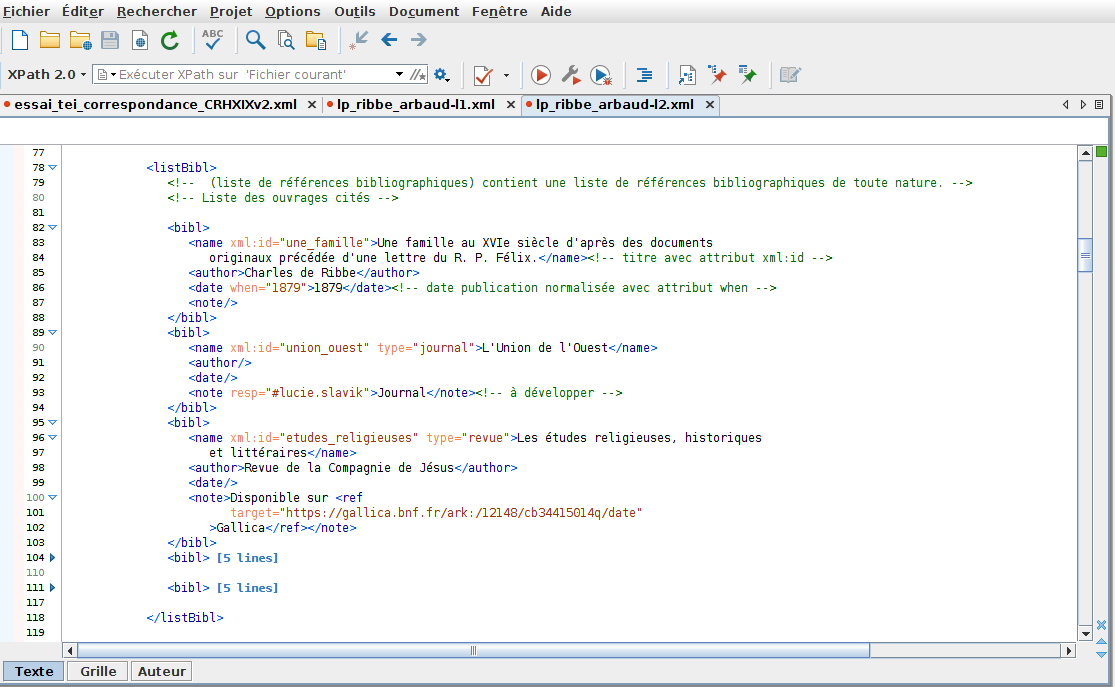
\includegraphics[width=16cm]{images/listBibl.png}
    \label{listBibl}
\end{figure}
À cet endroit, on pourra donner des informations sur l'ouvrage en question. La note pourra comporter un attribut \citecode{@resp} pour indiquer qui en est l'auteur. Cela permettra également de hiérarchiser la qualité des commentaires. Une note rédigée par un étudiant stagiaire sera considérée de moindre valeur que celle d'un spécialiste de Le Play.

La balise \citecode{<name>} doit obligatoirement avoir un attribut \citecode{@xml:id} qui permettra de pointer dans le texte vers l'index.

Par ailleurs, la balise \citecode{<author>} ne sera pas utile pour les journaux. Elle sera donc facultative pour les journaux mais obligatoire pour les ouvrages, distinction qui ne sera pas mentionnée dans l'ODD mais qui est néanmoins importante à avoir en tête.

La balise \citecode{<ref>} avec attribut \citecode{@target} permet de faire un lien vers un site\footnote{À confirmer, nous n'avons pas encore eu l'occasion de le tester.}. 

\subsubsection{L'index des événements}

Toujours dans le \citecode{<sourceDesc>}, après l'index des ouvrages, on trouve l'index des événements, sous la balise \citecode{<listEvent>}. Il recense les événements importants qui sont mentionnés dans la correspondance. Chaque événement marquant est contenu dans une balise \citecode{<event>} avec un attribut \citecode{@when} mentionnant la date normalisée. La balise \citecode{<event>} englobe un \citecode{<label>} contenant le titre de l'événement et comportant un attribut \citecode{@xml:id} indispensable pour qu'on puisse faire référence à l'événement dans le corps du texte. On peut laisser un commentaire sur l'événement dans une balise \citecode{<note>}, avec un attribut \citecode{@resp} indiquant par qui elle a été rédigée.

Les autres index se trouvent dans le \citecode{<profileDesc>}.

\subsubsection{L'index des noms de lieu}
Le \citecode{<settingDesc>} comprend l'index de noms de lieu.
Les informations sur le lieu sont encadrées d'une balise \citecode{<place>} qui a un attribut \citecode{@ xml:id} indispensable pour pointer ensuite du texte vers l'index. Dans le \citecode{<placeName>} est renseigné le nom du lieu, dans \citecode{<country>} le pays, dans la \citecode{<note>}, on peut écrire la description que l'on veut. On peut donc y glisser les notes rédigées par les transcripteurs, ce que nous n'avons pas pris le temps de faire durant les tests d'encodage des premières lettres en XML-TEI. Là encore, il y a possibilité d'y ajouter un attribut \citecode{@resp} pour renseigner qui a écrit la note.


\subsubsection{L'index des noms de personne}

Le \citecode{<particDesc>} (toujours dans le \citecode{<profileDesc>} comprend l'index des noms de personne et personnage mentionnés dans la correspondance. L'index est dans le \citecode{<listPerson>}. 

Pour chaque personne ou personnage, il y a une balise englobante \citecode{<person>} avec un attribut \citecode{@sex} pour indiquer le genre de la personne et un attribut \citecode{@xml:id} indispensable pour lui donner un identifiant qui permettra ensuite dans le texte de pouvoir pointer vers l'index. Le prénom suivi du nom sont indiqués dans la balise \citecode{<persName>}. Une balise \citecode{<note>} permet de présenter la personne en question, mais c'est une présentation générale qui n'est pas liée à une lettre en particulier. Si l'on veut faire une note adaptée à un endroit d'une lettre en particulier, il faut la mettre dans le corps du texte. Pour la \citecode{<note>}, on peut mettre un attribut \citecode{@resp} pour indiquer qui l'a écrite. Pour son contenu, il serait intéressant de réfléchir à une façon plus ou moins normée d'écrire les notes (prénom, nom, titres, dates de naissance et de mort, rôle dans la société en général, avec la sociologie en particulier et lien avec Le Play), ou reprendre tout simplement les normes indiquées par Monsieur Matthieu Brejon de Lavergnée\footnote{Voir 5.2.3 Des choix éditoriaux à faire en amont.}.

\subsubsection{L'index des noms d'organisation}

Le \citecode{<particDesc>} (toujours dans le \citecode{<profileDesc} comprend aussi l'index des noms d'organisation dans le \citecode{<listOrg>}. On peut si l'on veut les regrouper par type d'organisation avec un attribut \citecode{@type}, et faire donc plusieurs index (par exemple, un index d'organisations sociologiques, un index d'organisations politiques, un index d'associations etc.). Mais nous pensons plutôt ne pas faire de distinctions entre les différentes organisations et donc nous limiter à un simple index général pour simplifier au maximum l'encodage, d'autant que le profit retiré ne serait pas si grand.

Le nom de l'organisation est compris dans la balise \citecode{<org>} comprenant l'attribut \citecode{@xml:id} pour son identifiant. La balise \citecode{<orgName>} indique le nom de la société, et la balise \citecode{<note>} (plutôt que \citecode{<desc>}, intialement choisie, mais modifiée dans un souci de simplification) permet de rentrer une note générale sur l'organisation en question.

\subsubsection{L'index leplaysien}

La balise \citecode{<textClass>} comprend tous les autres index. En l'occurrence, il s'agit pour nous de l'index leplaysien. Les mots à indexer sont en cours de choix, la plupart ont été sélectionnés par Messieurs Antoine Savoye, Rémy Hême de Lacotte et Matthieu Brejon de Lavergnée mais il est nécessaire d'y réfléchir encore. Par exemple, nous avons distingué \inquote{ Réforme} de \inquote{Réforme morale} et \inquote{Réforme sociale}. Il serait bon de voir si l'on continue à distinguer ou si l'on met tout sous la même balise, avec le même identifiant \citecode{@xml:id}.

Quoiqu'il en soit, voici comment se présente l'index : on met tout d'abord une balise \citecode{<textClass>} comprenant une balise \citecode{<keywords>} comprenant elle-même une balise \citecode{<list>} avec, pour valeur de l'attribut \citecode{@type}, le nom de l'index dont il est question.

Chaque balise \citecode{<item>} comprend le nom du terme leplaysien avec un attribut \citecode{@xml:id} qui permettra de pointer vers le terme depuis le texte. Une balise \citecode{<note>} permet d'y laisser des commentaires. Il sera possible d'y ajouter un attribut \citecode{@resp} pour indiquer qui en est l'auteur.

Chaque \citecode{<keywords>} ouvrant un index, si l'on avait besoin de faire un autre index, on pourrait le mettre à cet endroit.\\

La réflexion autour de l'indexation a donc été riche. Nous avons d'ailleurs fait appel aux conseils de Monsieur Antoine Savoye, spécialiste de Le Play, pour nous éclairer quant au vocabulaire leplaysien à indexer.

\subsection{La normalisation}

Un des points importants dans XML est la normalisation. Nous l'avons déjà évoqué. Pour ELICOM, nous nous sommes surtout attachée à normaliser, outre les dates (\citecode{AAAA-MM-JJ}), les noms de personne dans le \citecode{<correspAction>}. 

Nous avons repéré en amont les destinataires des différentes correspondances, puis nous avons cherché s'ils étaient présents sur \emph{data.bnf}. En effet, sur \emph{data.bnf}, on trouve des fiches de référence sur les auteurs, les œuvres et les thèmes, et renvoyer à ce site permet l'interopérabilité\footnote{Voir \emph{Accueil}, Site web data.bnf, URL : \url{https://data.bnf.fr/} (visité le 17/06/2020).}.
\begin{figure}[ht]
    \centering
    \caption{La normalisation du \citecode{<correspAction>}, correspondance de Lamartine (\citecode{lamartine-col-vol1-12.xml}), capture d'écran d'Oxygen XML Editor}
    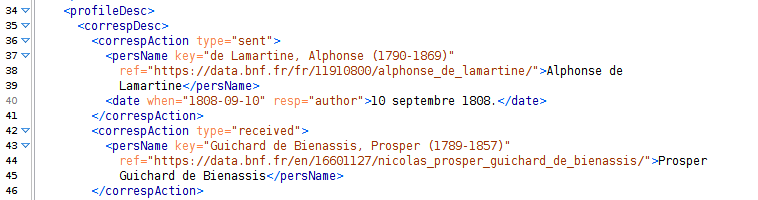
\includegraphics[width=16cm]{images/normalisation.png}
    \label{normalisation}
\end{figure}
Cependant, tous n'étaient pas rencensés dans \emph{data.bnf} notamment parmi les correspondants de Félicité de Lamennais et de Proudhon. Lorsque c'était le cas, nous avons donc supprimé l'attribut \citecode{@ref} renvoyant à \emph{data.bnf} et nous avons mis des parenthèses vides \citecode{(...-...)}, à la place des dates de naissance et de mort, en espérant pouvoir les remplir un jour\footnote{Voir dans les livrables, les dossiers de remarque des différentes correspondances du Labex OBVIL.}.\\


\section{L'ODD et la pérennité des données}

\subsection{Un schéma et une documentation pour la pérennité des données}
Une fois les balises XML définies, il s'agit de créer une documentation dessus pour expliquer nos choix. Or, il existe une technologie qui permet de gérer à la fois le schéma de balises et sa documentation, c'est un document qui fait tout, autrement dit \emph{One document does it all} (ODD).

Tout d'abord, comme le souligne Lou Burnard, \inquote{l'ODD est le langage de définition et de maintenance du système TEI. Il permet la maintenance du code et de sa documentation d’une manière intégrée, à partir d’une seule source XML. Il [...] fournit une manière efficace d’assurer la pérennité [des] données, en [...] obligeant de documenter leur usage d’une manière standardisée}\footnote{Lou Burnard, \emph{Comment maîtriser le tigre TEI}, URL : \url{https://cahier.hypotheses.org/files/2018/08/ODD-diapos.pdf} (visité le 11/06/2020).)}.

En bref, l'ODD comprend : 
\begin{itemize}
    \item Un schéma formel. Pour nous, nous avons choisi un schéma RELAX NG. Il contrôle l'édition, détermine quelles sont les balises disponibles, dans quels contextes, avec quels attributs, avec quelles valeurs, en respectant les contraintes et enchaînements. Nous y avons déjà réfléchi plus haut. 
    \item Une documentation pour expliciter aux utilisateurs et développeurs les principes éditoriaux, les principes de choix de balises etc. Nous l'avons fait dans XML puis nous l'avons édité dans un format HTML.
\end{itemize}
La figure ci-dessous\footnote{Fig. 10.9} permet de mieux saisir ce qu'est l'ODD\footnote{J.B. Camps, \emph{ODD Structuration des données et des documents : balisage XML. Personnaliser la TEI : One Document Does it all}, M2 TNAH, ENC, 2017, p.44 URL : \url{https://halshs.archives-ouvertes.fr/cel-01706530/file/06_TEI_ODD_Camps_20170202.pdf} (visité le 12/06/2020).}. Elle résume nos propos.
\begin{figure}[ht]
    \centering
    \caption{L'ODD}
    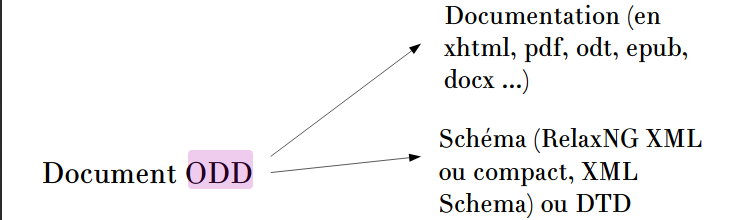
\includegraphics[width=16cm]{images/ODD.png}
    \label{ODD}
\end{figure}

\subsection{Créer l'ODD et l'associer à un document XML-TEI}

Un ODD est un document TEI. Pour ce qui est du projet Le Play, nous l'avons construit avec oXygen XML Editor. Pour faciliter sa construction, nous avons utilisé \emph{ODD By Example}\footnote{Pour plus d'informations sur le scénario \emph{oddbyexample}, voir Ariane Pinche, Séance 11, \inquote{Personnaliser son ODD}, Cours M2 TNAH, URL~: \url{https://github.com/ArianePinche/coursTNAH_XML-TEI/tree/master/seance11} (visité le 18/02/2020).}.

Après avoir installé notre scénario \emph{oddbyexample}, nous avons transformé l'0DD en RELAX NG, puis nous avons associé le schéma RELAX NG au fichier XML-TEI. Ainsi, l'association de l'ODD et du fichier XML-TEI se fait via le fichier RELAX NG. 

Une fois que notre fichier TEI est lié au schéma qui le contraint, il doit lui correspondre. Dès qu'un enchaînement de balises, contraint dans le schéma, n'est pas respecté, le fichier XML-TEI le signale : cela pousse donc à une certaine rigueur. Par ailleurs, si l'on a des doutes sur la façon d'encoder, on peut toujours se reporter à l'ODD qui explique les choix. Ainsi, si la personne qui encode se rend compte d'une erreur, elle peut modifier et mettre à jour l'ODD, en indiquant que c'est elle qui a fait la modification. 

\begin{figure}[ht]
    \centering
    \caption{Extrait de la table des matières de l'ODD pour le projet Le Play}
    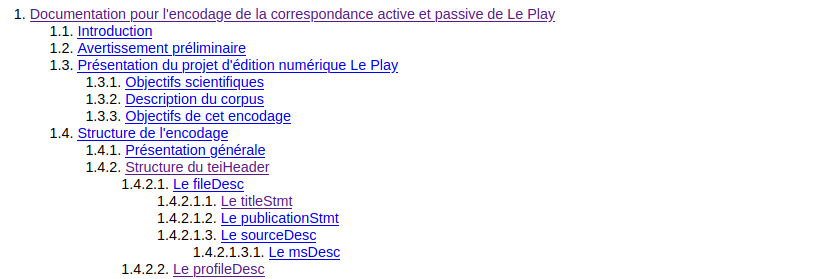
\includegraphics[width=16cm]{images/tableMatiereODD.png}
    \label{tableMatiereODD}
\end{figure}

\subsection{L'ODD dans nos projets}

Nous avons eu un rôle très différent quant à l'ODD pour nos deux projets. Pour ELICOM, l'ODD n'avait pas encore été réalisé. Nous n'avons donc été chargée que du travail en amont. En effet, avant de réaliser l'ODD, il faut avoir une connaissance assez large du corpus. Néanmoins, il a été parfois difficile pour nous de ne pas avoir d'ODD auquel nous pouvions nous référer pour garder une cohérence et une constance dans le choix des balises.

Pour le projet Le Play, c'est nous qui avons été chargée de la mise en place de l'ODD. Nous avons donc été au c\oe ur de certains choix. Néanmoins, il est à noter que cet ODD est encore perfectible. De nombreux cas n'ont pas encore été traités. C'est donc un document susceptible d'être modifié. Nous pensons notamment à l'encodage des documents joints à certaines lettres ainsi que nombre d'autres cas particuliers que nous n'avons pas eu le temps de traiter durant ce stage relativement court.
Il sera donc nécessaire de mettre l'ODD du CRHXIX à jour, au fil des cas particuliers rencontrés\footnote{Notre ODD pour le CRHXIX est joint à nos livrables.}.

L'ODD est donc un incontournable pour qui veut encoder des données en XML-TEI, de façon cohérente et pérenne.

XML a donc été le langage de base dont nous nous sommes servies pour nos éditions numériques de correspondance. Néanmoins, nous avons eu également recours à d'autres technologies.

\section{Au service d'XML}

\subsection{XSLT}

XSLT est un langage basé sur XML, permettant de styliser ou transformer des fichiers XML ou HTML. Comme nous l'avions déjà souligné dans la troisième partie\footnote{Voir 9.6.2 La question des \emph{tags}} nous aurions pu passer par une feuille de transformation pour passer du fichier XML-TEI exporté de Transkribus et criblé de fautes, à un fichier XML-TEI comportant les noms de balises conformes. Cela reste une possibilité mais pour notre part, nous n'avons pas poussé plus loin la réflexion. En revanche, nous avons eu recours au langage de programmation Python. 

\subsection{Python}

\subsubsection{Un \emph{script} Python pour extraire les fichiers XML}

Dans le cadre du projet ELICOM, Python nous a servi à extraire du résultat de l'OCR, le texte des différentes lettres pour les encoder en XML-TEI dans des fichiers séparés\footnote{Le \emph{script} Python sert à la fois à distinguer les lettres les unes des autres et à passer en TEI.}.

Pour cela, nous avons installé un environnement virtuel basé sur Python 3 avec plusieurs \emph{packages} dont \textbf{lxml} qui est un parseur pour les fichiers XML et HTML en Python, utilisé ici pour construire les fichiers XML,  ainsi que \textbf{beautifulsoup4} \inquote{qui permet une interaction simplifiée en Python avec les fichiers XML et HTML parsés}\footnote{Voir Alix Chagué, \emph{Ibidem}, p.85}. Par ailleurs, BeautifulSoup fonctionne sur les fichiers HTML mal formés, ce qui est le cas ici. Nous avons également importé le module \textbf{re} pour faire des regex dans Python.\\

Un \emph{script} Python avait déjà été réalisé par un membre de l'équipe du Labex OBVIL\footnote{Voir Fig. 10.11}. Nous avons donc eu un squelette commun, une base commune traitant les points communs aux différents corpus, mais à adapter à chacun. En effet, chaque corpus est tout de même à traiter différemment car les données n'apparaissent pas toujours de la même manière, à cause des différentes stratégies d'édition.

\begin{figure}[ht]
    \centering
    \caption{Extrait du \emph{script} \citecode{extraction-elicom.py}, capture d'écran de Sublime Text}
    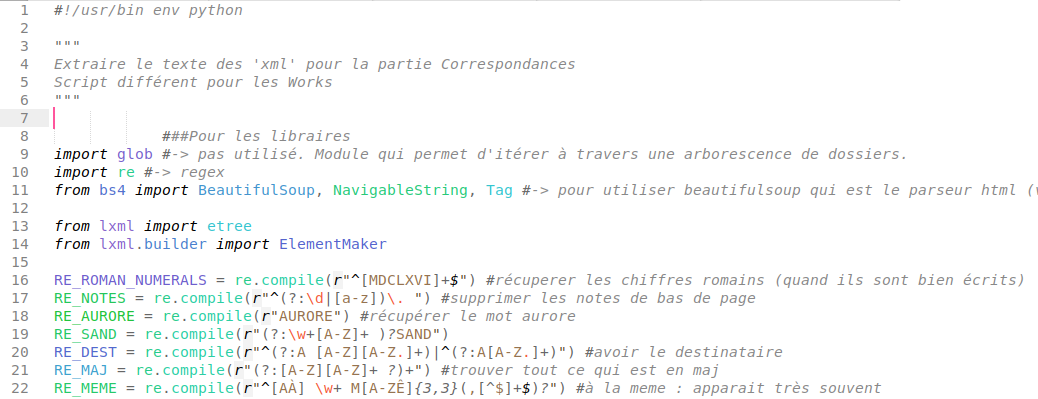
\includegraphics[width=15cm]{images/extraction.png}
    \label{extraction}
\end{figure}

\subsubsection{Les regex dans Python}

Avec les regex dans python, nous nous sommes surtout attachée à matcher les chiffres romains pour Lamartine, les chiffres arabes pour Lamennais, et les signatures pour Proudhon, afin de pouvoir extraire les lettres\footnote{Voir 8.2.5 Premiers repérages des marqueurs : pour Lamartine, les lettres sont toujours introduites par des chiffres romains, pour Lamennais par des chiffres arabes. Pour Proudhon, nous nous sommes servie de sa signature.}.

On peut constater sur la figure ci-dessus\footnote{Fig. 10.11} que les lettres de George Sand (\emph{script} \citecode{extraction-elicom.py}) ont été aussi extraites au moyen du repérage des chiffres romains via une regex.
\begin{figure}[ht]
    \centering
    \caption{Extrait du \emph{script} de Proudhon, capture d'écran de Github}
    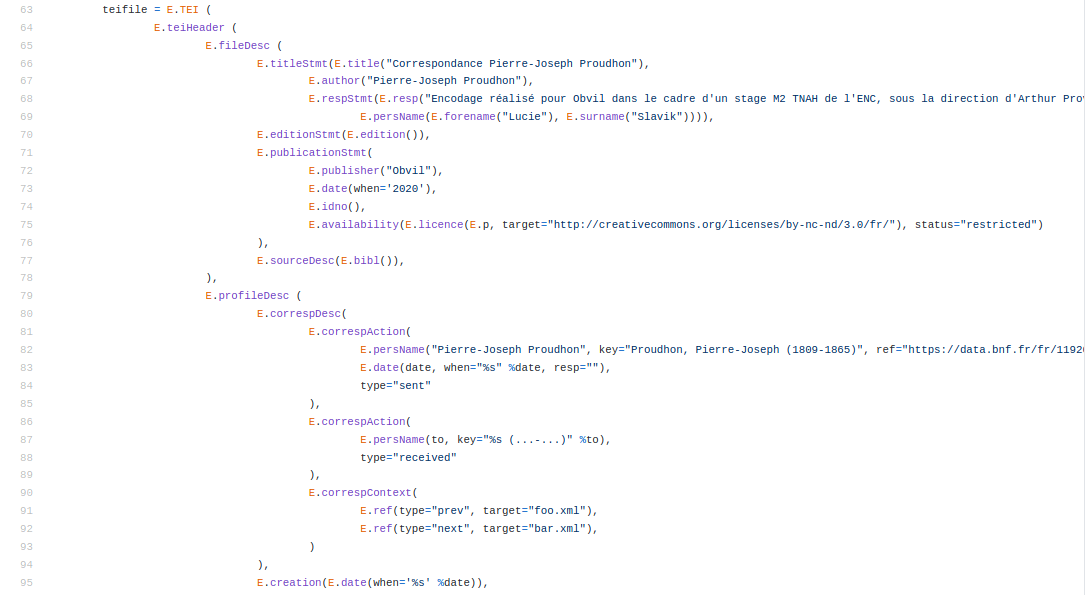
\includegraphics[width=15cm]{images/scriptProudhon.png}
    \label{scriptProudhon}
\end{figure}

Ainsi, à chaque chiffre arabe ou romain ou signature, une lettre était extraite et mise directement en XML-TEI grâce au module \textbf{lxml.builder}. La figure ci-dessous\footnote{Fig. 10.12} montre l'arborescence demandée depuis le \emph{script} Python de Proudhon.\\

Par ailleurs, nous nous sommes également servie des expressions régulières pour extraire les métadonnées et les récupérer ensuite dans le \citecode{<teiHeader>}. Par exemple, pour le \emph{script} de Proudhon, nous avons écrit \citecode{RE\_DEST = re.compile(r"A M\. [A-Z].+")} pour matcher les destinataires de Proudhon, et \citecode{RE\_DATE = re.compile(r"([\^,]+), (.+)\$")} pour matcher la date d'écriture de la lettre, puis nous avons mis ces informations dans le \citecode{<teiHeader>}\footnote{Voir les \emph{scripts} dans leur intégralité dans les livrables.}. 

\subsubsection{Les limites de l'OCR entravent l'efficacité du \emph{script} Python}

Cependant, tout n'est pas parfait du premier coup. Certes, Python nous avance beaucoup et fait gagner beaucoup de temps dans l'extraction des lettres et leur transformation en fichiers XML-TEI en vue de leur édition. Toutefois, certaines choses restent à modifier.

Tout d'abord, certaines modifications doivent parfois être faites en amont pour une meilleure extraction : c'est le cas lorsque des chiffres arabes ou romains ont été mal océrisés et empêchent la regex de les reconnaître : ainsi, les fautes de l'OCR rendent l'extraction difficile.

Par ailleurs, après l'application du \emph{script}, on remarque également certaines défaillances, encore dûes à la mauvaise océrisation. En effet, nous avons élaboré pour la correspondance de Lamennais une regex afin de matcher et supprimer les notes de bas de pages qui étaient disséminées au sein du texte. Des centaines de notes ont été ainsi supprimées. 
\begin{figure}[ht]
    \centering
    \caption{Lettre de Lamennais, notes mal matchées à cause de l'océrisation, \citecode{lamennais-cor-vol1-112.xml}}
    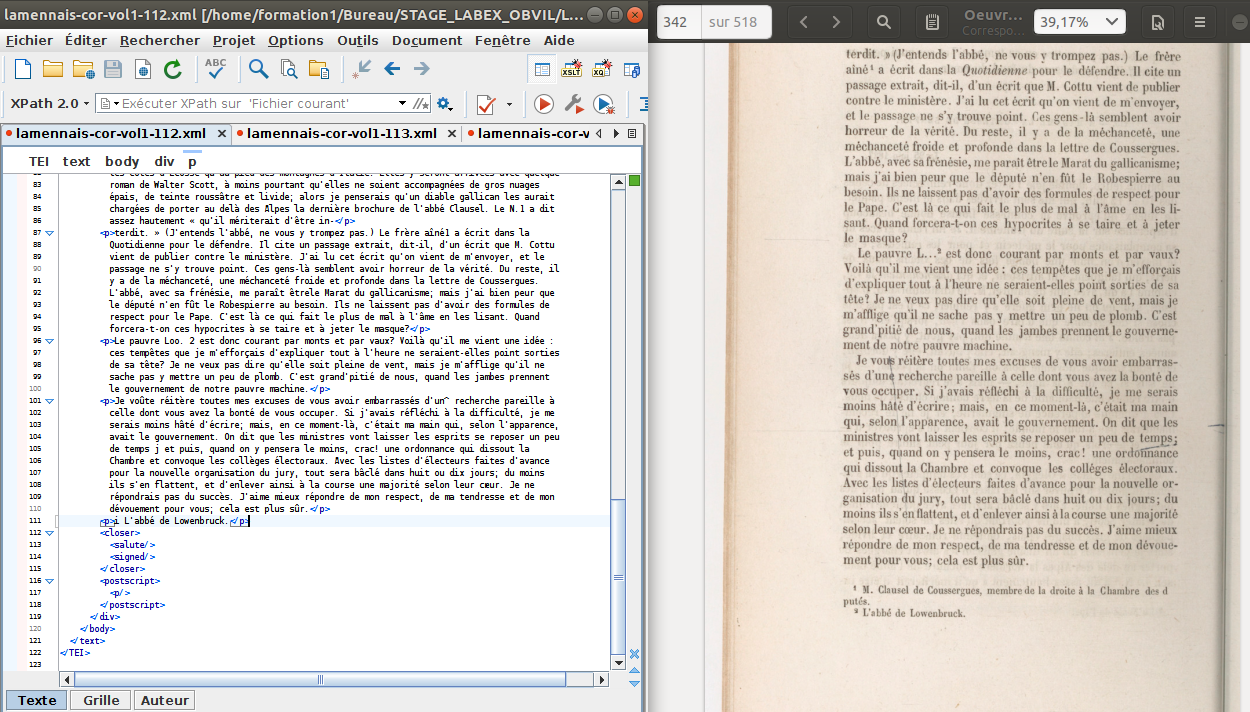
\includegraphics[width=16cm]{images/notesLamennais.png}
    \label{notesLamennais}
\end{figure}
Cependant, de nombreuses notes n'ont pas été matchées par la regex (et ont donc échappé à la suppression) car l'océrisation avait été mauvaise. L'exemple de la figure 10.13 est typique : on constate que la première note a été supprimée mais que la deuxième subsiste : le \inquote{2} a été pris pour un \inquote{i} par l'OCR. La note n'a donc pas été matchée et il faut donc la supprimer autrement\footnote{Pour notre part, nous l'avons fait manuellement.}.

Enfin, le résultat de l'OCR n'étant balisé que par des \citecode{<p>} et des \citecode{<span>}, et qu'aucune autre indication stylistique ou bien de structure n'apparaît, cela empêche un traitement plus fin des données pour la mise en page ou le signalement des vers. Ainsi, l'OCR ne tient pas compte des italiques, mais nous n'avons pas traité ce point. En revanche, pour ce qui est de la mise en page, nous nous sommes penchée sur la question : Lamartine surtout et parfois Lamennais glissaient des vers dans leurs lettres. Pour Lamartine, c'était assez fréquent. Il lui arrivait même parfois d'écrire une lettre intégralement en vers\footnote{La lettre 38 par exemple.}.

Afin de les remettre en valeur, nous avons choisi d'indiquer les strophes par les \citecode{<lg>} et les vers par les \citecode{<l>}, pour améliorer les repérages et la visualisation, dans le but de poursuivre l'objectif de cette édition numérique qui veut permettre une plus grande facilité d'accès au texte pour y effectuer des recherches plein texte et sur la structure, via l'interrogation des balises et des métadonnées.

Pour effectuer ce travail, nous avons dû mettre en regard les numérisations pour voir quelles lettres contiennent des vers. Nous avons donc fait ces ajouts manuellement.
\begin{figure}[ht]
    \centering
    \caption{Mise en place des \citecode{<lg>} et des \citecode{<l>} dans la correspondance de Lamartine}
    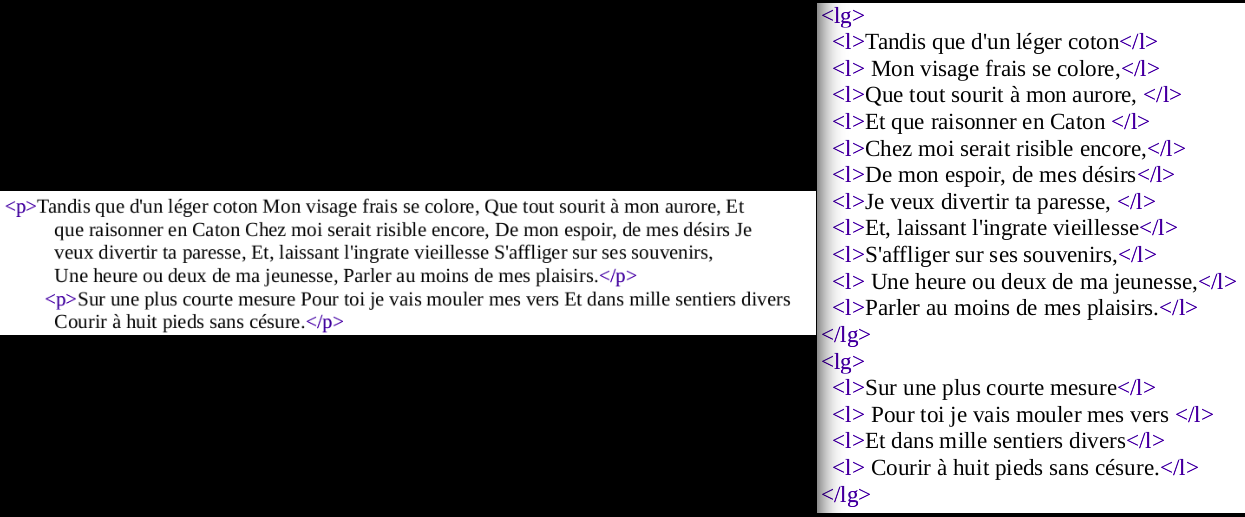
\includegraphics[width=16cm]{images/lamartineLG.png}
    \label{lamartineLG}
\end{figure}
On peut constater sur la figure 10.14 les modifications qui ont été faites. Sur la gauche, on voit le fichier XML qui a été extrait : les deux strophes apparaissent dans deux paragraphes (\citecode{<p>}), sans aucune distinction des vers. Sur la droite, les deux paragraphes sont devenus des strophes reconnues par les \citecode{<lg>}, et au sein des strophes, chaque vers (\citecode{<l>}) est marqué par un retour à la ligne.\\

XML est donc poussé au bout de ses possibilités avec l'apport d'autres technologies telles que Python, XSLT et les regex. Néanmoins, la qualité pas toujours optimale de l'OCR nécessite tout de même de nombreuses reprises à la fois techniques et orthographiques. 

Toutes ces technologies sont donc au service de l'édition numérique de correspondance et elles permettent de traiter les données acquises.



\chapter{Relever les défis du projet numérique}

\section{Des difficultés à surmonter}

Nous avions déjà évoqué plus haut\footnote{6.6 Le cahier des charges} les difficultés que rencontrent nombre de projets numériques, que cela soit dans le public ou le privé : deux tiers rencontrent de gros problèmes au cours de leur élaboration, et un tiers se solde par un échec\footnote{Voir Jean-Louis Foucard, Module de formation \inquote{Manager un projet Numérique} \inquote{Master Archives – Technologies numériques appliquées à l’histoire}, École Nationale des Chartes, mars 2020.}.

Nos deux projets n'échappent donc pas à cette constante. Pour ce qui est du projet au CRHXIX, nous pensons que le manque de subventions pourrait être un des freins au développement du projet, qui toutefois avance peu à peu. 

Pour ELICOM, nous n'avons pas assez de recul pour voir les difficultés que nous pourrions rencontrer. Une fois que l'ODD sera faite, ce sera bien-sûr un grand pas en avant, tant pour éclairer l'encodage que pour la pérennité des données.\\

Pour prévenir les difficultés, notre rôle en tant que stagiaire a été d'être un relais et d'assurer la transmission de notre travail, d'autant que nous avons réalisé la totalité de notre travail sur nos deux projets en télétravail. 

\section{Prévenir le \inquote{facteur d'autobus}}

Pour la réussite d'un projet, il s'agit d'éviter ce que les britanniques appellent le \emph{bus factor}, autrement dit, le \inquote{facteur d'autobus}, expression qui vient de la phrase \inquote{Combien de personnes clés dans votre équipe peuvent se faire renverser par un autobus avant que votre projet échoue ?}. Ainsi, \inquote{le ``facteur d'autobus'' est le nombre minimum de membres de l'équipe qui peuvent disparaître soudainement d'un projet avant que celui-ci ne s'arrête par manque de personnel compétent ou bien informé}\footnote{\emph{Facteur d'autobus}, Wikipédia, URL : \url{https://fr.wikipedia.org/wiki/Facteur_d\%27autobus} (visité le 28/09/2020).}.

Autrement dit, en tant que stagiaire, il faut qu'une fois que nous avons quitté le projet, les membres de l'équipe, que ce soit celle du CRHXIX ou du Labex OBVIL, aient en main tout notre travail et puisse profiter de ce que nous avons appris, compris, repris durant notre stage. Il s'agit d'assurer la transmission des savoirs et le transfert de compétences. 

\subsection{Les avantages de GitHub}

Pour cela, GitHub est un moyen intéressant pour le travail en équipe et la transmission. GitHub est un \inquote{service web d'hébergement et de gestion de développement de logiciels, utilisant le logiciel de gestion de versions Git}\footnote{\emph{GitHub}, Wikipédia, URL : \url{https://fr.wikipedia.org/wiki/GitHub} (visité le 28/09/2020).}. Il permet donc le versionnage\footnote{On entend par versionnage la \inquote{Gestion des différentes versions d'un même document}. Voir \cite{versionnage}} ainsi que le travail en équipe avec le partage de code.
Nous ne l'avons pas utilisé pour le projet Le Play mais pour le projet ELICOM\footnote{Voir OBVIL/Elicom, Github, URL : \url{https://github.com/OBVIL/elicom}}. Nous avons donc pu transmettre notre travail au fur et à mesure et faire des rapports au jour le jour pour une meilleur gestion de projet. À cela se sont ajoutés les appels réguliers avec le tuteur technique pour faire le point, et un rapport général en fin de stage.

Si nous n'avons pas usé de cette stratégie pour notre travail au CRHXIX, des contacts fréquents avec l'équipe, aussi bien par courriel que par téléphone ou encore par visioconférence ont eu lieu. Le transfert du travail se fera sous peu. Par ailleurs, pour le transfert de compétences, nous avons mis en place des tutoriels.

\subsection{Des tutoriels et des fiches de savoir pour assurer la transmission}

Ainsi, pour le CRHXIX, nous avons constitué divers tutoriels selon les technologies utilisées, afin que les membres de l'équipe puissent prendre la suite de la partie numérique.\\

Pour ce qui est de notre travail sur Transkribus, nous avons réalisé quatre tutoriels, pour chaque étape :

\begin{itemize}
    \item Un premier tutoriel pour le chargement des données et leur premier traînement\footnote{Voir dans les livrables \citecode{Tuto1\_preparation\_des\_donnees\_transkribus.pdf}}
    \item Un second dédié à l'entraînement du modèle \footnote{Voir dans les livrables \citecode{Tuto2\_entrainement\_du\_modele.pdf}}
    \item Un troisième consacré à l'application du modèle définitif \footnote{Voir dans les livrables \citecode{Tuto3\_application\_du\_modele.pdf}}
    \item Un quatrième qui traite de l'exportation des données depuis le serveur Transkribus \footnote{Voir dans les livrables \citecode{Tuto4\_exportation\_transkribus.pdf}}
\end{itemize}

Par ailleurs, nous avons réalisé un point sur notre travail pour dire où nous en étions et quelles conclusions nous tirions de cette première expérience\footnote{Voir dans les livrables \citecode{point\_transkribus.odt}}.\\

Pour ce qui est de notre travail sur XML-TEI et ODD, nous avons également travaillé à la transmission, pour le CRHXIX : 
\begin{itemize}
    \item Par la réalisation d'un tutoriel\footnote{Voir dans les livrables \citecode{Tuto\_XML-TEI\_CHRXIX.pdf}} pour la prise en main d'Oxygen XML Editor afin de réaliser les encodages
    \item Par la transmission d'un tutoriel sur l'ODD\footnote{Ce tutoriel n'a pas été réalisé par nos soins en revanche.}.
\end{itemize}
Par ailleurs, la documentation de l'ODD\footnote{L'ODD du CRHXIX est disponible dans les livrables.} est le moyen par excellence pour prévenir le \inquote{facteur d'autobus}. Nos choix y sont justifiés, et nos questionnements son présentés. Celui qui prendra la suite du projet pourra donc comprendre la logique de notre travail, perfectionner l'ODD et résoudre certains problèmes ou questionnements.

Quant à ELICOM, nous avons, au fur et à mesure de notre travail, constitué des fichiers rassemblant nos remarques sur l'HTML et le XML et à l'occasion du \emph{script} Python de chacun des auteurs. Nous y avons entre autres écrit quelques expressions régulières. Ces fichiers sont perfectibles et auraient pu être perfectionnés. Nous avons quand-même choisi de les mettre dans les livrables à titre d'exemple. À la fin de notre travail sur Lamartine, nous avons également réalisé un fichier récapitulatif sur le code Python.\begin{figure}[ht]
    \centering
    \caption{Rapport sur le code Python de Lamartine, capture d'écran de GitHub}
    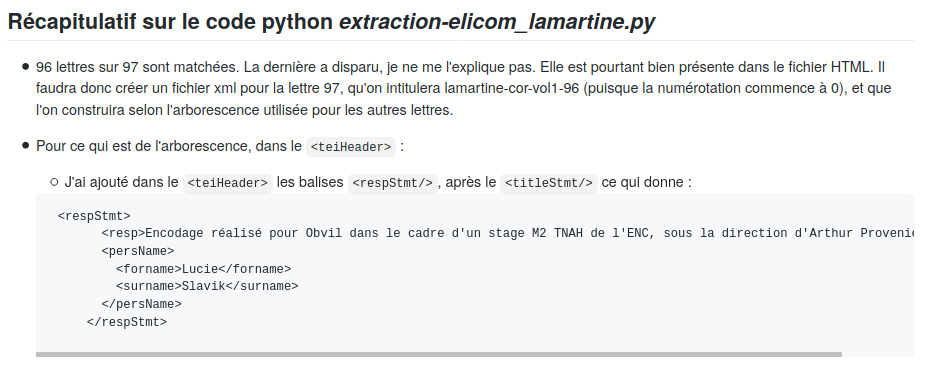
\includegraphics[width=16cm]{images/recapLamartine.png}
    \label{recapLamartine}
\end{figure}
Celui-ci est disponible sur GitHub\footnote{Voir \url{https://github.com/OBVIL/elicom/blob/master/extraction_cor_stage2020/cor_lamartine/remarques/recapitulatif_lamartine.md}}. La figure ci-dessus\footnote{Fig. 11.1} donne un échantillon de ce rapport rédigé au moyen du langage de balisage Markdown.\\

Par ailleurs, le cahier des charges du CRHXIX ayant été un peu détourné de sa fin en se transformant en rapport, il a toutefois permis également de faire un petit bilan de la situation pour voir où nous en étions et quelles étaient les prochaines étapes à suivre. \\

Enfin, nous avons réalisé des fiches pour accélérer certaines normalisations. Ainsi, pour le CRHXIX, nous avons écrit sept fiches pour les normalisations des index, que ce soit pour le recensement des correspondants dans le \citecode{<teiHeader>} ou les six index.

De même, pour ELICOM, nous avons constitué des index de correspondants pour pouvoir normaliser plus facilement chacun des destinataires lors des corrections des fichiers XML.

\subsection{Documenter son code}

Enfin, un des moyens d'assurer la transmission est la documentation du code en direct. En effet, pour ce qui est des \emph{scripts} Python pour ELICOM, nous avons essayé, du moins au début, de bien documenter notre code, à la fois pour mieux le comprendre et aussi pour mieux le faire comprendre. Cela fait partie des bonnes pratiques pour nos projets numériques. De même pour les premiers essais d'encodage en XML-TEI pour le CRHXIX, nous avons commenté chaque balise pour la justifier et l'expliquer. Nous avons été particulièrement attentive à cela dans un souci de transmission, et ceci nous a d'ailleurs aidée nous-même au moment de la rédaction de l'ODD car il n'y avait plus qu'à suivre les indications déjà présentes dans les fichiers XML commentés au fur et à mesure.\\


Nous avons donc tenté de relever au cours de nos stages les défis de ces deux projets d'édition numérique de correspondance sur des corpus du XIX\up{e} siècle. Cette partie de traitement des données s'est réalisée autour du langage XML, avec le souci de transmettre non seulement les réalisations de notre travail mais également les étapes de réflexion par lesquelles nous sommes passée.

\part*{Conclusion}
\addcontentsline{toc}{part}{Conclusion}
\markboth{Conclusion}{Conclusion} 

Nos deux stages nous ont permis d'approfondir les enjeux de l'édition numérique de correspondance par deux approches différentes, sur des corpus du XIX\up{e} siècle. Cette double expérience nous a permis d'avoir une vue plus large et de découvrir différents projets auxquels nous avons pris plaisir à participer.

Dans une première partie, nous nous sommes penchée sur les contextes des projets, les buts qu'ils se proposent, et la matière première si l'on peut dire, sur laquelle ils se basent pour atteindre les objectifs fixés. Ces éléments sont essentiels pour avoir une meilleure vue d'ensemble des projets et cerner ensuite quel rôle sera le nôtre, comment nous nous inscrivons dans ces projets, et quels moyens prendre pour y contribuer et les faire avancer .
Nous avons donc analysé le contexte universitaire et intellectuel des projets : notre but est de faire avancer la recherche historique et culturelle en général. Cependant, ces deux projets, bien que travaillant tous deux à la diffusion de correspondances du XIX\up{e} siècle, diffèrent dans leur but. Certes, ils ont les points commun du genre épistolaire et du cadre dans lequel les lettres ont été produites, le XIX\up{e} siècle, mais le CRHXIX \oe uvre à une édition plus classique, centrée sur une personne autour de laquelle se greffe un réseau de correspondants, le but restant la recherche historique, alors que pour le Labex OBVIL, ELICOM est un moyen de pousser les possibilités du numérique en terme de fouilles de données, d'enrichissement et de visualisation, ainsi que la recherche en humanités numériques, avec un séminaire de recherche consacré au projet et aux avancées de l'édition numérique de correspondance.
Bien sûr, certains outils restent les mêmes, mais l'optique est différente.
Cette différence s'accentue lorsque l'on considère les sources qui servent de point de départ aux deux projets. Pour le CRHXIX, nous avons affaire à des manuscrits originaux, qui ont été numérisés ou devront l'être.
Certes, nous n'avons pas accès directement à la source mais à son fac-similé. Nous sommes néanmoins assez proches de l'original.
Par ailleurs, nous ne nous appuyons aucunement sur des éditions précédentes, en ce sens-là, notre travail d'édition est conséquent puisque nous ouvrons la voie. Pour ELICOM, au contraire, nous travaillons sur des sources indirectes. Nous n'avons pas accès aux manuscrits ni à des fac-similés mais à de précédentes éditions imprimées. Nous prenons de la distance avec elles dans les notes et certains choix, mais elles restent tout de même notre point de départ. Notre rapport à la source est donc différent, dans l'un et l'autre projet. Or, la source a son rôle dans le choix des moyens car on les adapte à elle. Ce sont ces considérations qui nous ont occupée pendant la première partie. 

Après avoir exposé nos projets et leurs différentes facettes, nous avons souhaité prendre un peu de hauteur par rapport à l'édition numérique de correspondance aujourd'hui, et faire un état de l'art : où en sommes-nous, quels sont les moyens mis à notre disposition ? 
Toutes ces réflexions vont influencer notre manière d'agir et d'aborder nos projets. Nous avons donc établi un petit bilan scientifique sur les réflexions de la communauté scientifique autour de l'édition numérique de correspondance, et les divers déploiements d'outils pour favoriser son essor. Nous avons abordé les problématiques propres à l'édition numérique de correspondance, sachant que l'aspect numérique est essentiel. 
Nos considérations sur l'édition numérique de correspondance se sont conclues par la pratique : nous avons donc envisagé notre futur site pour le CRHXIX, concluant ainsi notre deuxième partie.

Après la théorie, nous sommes donc passée à la pratique, tout d'abord pour ce qui est de l'acquisition des données, ce qui a fait l'objet de notre troisième partie. Or, ici, nous avons constaté que pour nos deux projets, la nouvelle technologie de l'apprentissage machine s'est avérée être au c\oe ur de l'acquisition des données, tant pour ELICOM via l'OCR de Gallica, que pour notre projet d'édition numérique de la correspondance de Frédéric Le Play, via l'HTR de Transkribus. Nous avons particulièrement développé ce point de Transkribus, outil de transcription collaborative fort utile. Néanmoins, des interrogations subsistent quant à la rentabilité du modèle, au traitement et au mode d'importation des données. Vaudrait-il mieux passer par XSLT ? Devrait-on penser davantage au \emph{tags} dans Transkribus et les personnaliser ? Ce sont autant de questions qui se posent encore. Quant à l'OCR de Gallica, nous avons pu voir qu'il conditionnait beaucoup le pré-traitement et traitement des données sur lequel nous nous sommes plus attardée en quatrième partie.

Après avoir considéré l'acquisition des données, nous nous sommes penchée sur leur traitement. Dans cette partie, nous avons vu combien le langage XML est utilisé dans les éditions numériques de correspondance. Celui-ci qui a, en soi, de multiples possibilités, est restreint en l'occurrence à nos besoins d'édition de correspondance. Nous avons donc expliqué nos choix de balises, leur documentation via l'ODD, ainsi que les technologies utilisées pour pousser au maximum les possibilités d'XML, à savoir XSLT - qui reste encore un moyen à utiliser éventuellement - et Python. Puis nous avons exposé les difficultés inhérentes aux projets numériques, les défis à relever, et les moyens que nous avons employés dans ce but, pour que les projets soient menés à terme. Nous n'avons été qu'un maillon de la chaîne, mais il ne doit pas manquer, au risque de briser cette chaîne.

Le contexte de télétravail a rendu l'expérience de ces stages particulièrement inédite. Nous avons dû relever le défi de travailler seule et de n'être reliée aux différentes équipes que par le net. Nous avons en quelque sorte travaillé avec des équipes qui nous ont paru un peu virtuelles, quoique toujours là pour répondre à nos questions.

Malgré tout, le bilan reste très positif. Nous avons pu mettre en pratique les connaissances reçues à l'ENC, et nous familiariser toujours plus aux diverses technologies. Nous avons particulièrement apprécié le fait de voir concrètement, dans des projets bien réels, les avantages et les possibilités du numérique. 

Pour ce qui est de notre stage au Labex OBVIL, au total, 388 lettres ont été extraites, dont 264 fichiers ont été corrigés durant ces 20 jours de stage. Nous avons donc eu la satisfaction d'avoir pu participer au projet ELICOM.
Dans l’ensemble, ce stage nous a bien aidée à consolider nos connaissances en XML et nous a indirectement aidée pour le projet Le Play, grâce à leur point commun d'édition de corpus épistolaires du XIX\up{e} siècle. Le plus grand défi de ce stage s'est situé dans la rédaction du code Python que nous avons appris à mieux maîtriser, même si de grands progrès restent à faire.

Quant à notre stage au CRHXIX, il a été extrêmement enrichissant car nous avons été chargée de penser la partie numérique du projet. Durant tout le confinement, nous avons été la seule personne de l'équipe, à quelques exceptions près, à pouvoir nous consacrer totalement à ce projet.
Sans les remarques du chef de projet et de membres de l'équipe, et sans l'aide des professeurs de l'École, particulièrement celle de notre tuteur, ainsi que le soutien de notre tuteur d'OBVIL, nous n'aurions pas pu aller aussi loin dans le projet. Durant une petite trentaine de jours, nous avons dû faire nôtre les enjeux du projet, prendre en main Transkribus qui nous était presque totalement étranger, entraîner un modèle avec plus de 20 000 mots, penser à l'exportation en XML-TEI, se faire une idée du futur site et en fonction, penser l'encodage en TEI. Cela a donc été un stage particulièrement riche par sa diversité. Il n'a pas été exempt de limites : nous n'avons pu réaliser de véritable cahier des charges ni de récits utilisateurs dignes de ce nom. Néanmoins, il était difficile de tout mener de front en si peu de temps.

Ces différentes approches de l'édition numérique de correspondance ont donc été très enrichissantes.
Nous avons pu constater que l’épistolaire à l’ère du numérique se situe réellement entre des perspectives historiques, ou plus largement des perspectives de sciences humaines, d'aide à la recherche et autres, et des innovations technologiques. Nous sommes entre les sciences humaines et le numérique, nous sommes tout simplement dans les humanités numériques, avec peut-être un aspect plus \inquote{humanités} pour le projet Le Play, et plus \inquote{numérique} pour ELICOM. 

Ainsi, ces projets sont l'illustration que les humanités numériques, comme le souligne le \emph{Manifeste des digital humanities}\footnote{\emph{Manifeste des digital humanities}, THATCamp, Paris, 2010 URL : \url{https://tcp.hypotheses.org/318} (visité le 29/09/2020)}, \inquote{ne font pas table rase du passé, mais s'appuient, au contraire, sur l'ensemble des paradigmes, savoir-faire et connaissances propres à ces disciplines, tout en mobilisant les outils et les perspectives singulières du champ du numérique}.


% annexes
\appendix
\part*{Annexes}
\addcontentsline{toc}{part}{Annexes}
\pagestyle{myheadings}
\markboth{Annexes}{Annexes}

Les annexes contiennent certaines illustrations du mémoire ainsi que la description des fichiers disponibles dans les livrables sur Github à cette adresse : \url{https://github.com/LaureRossignol96/MemoireTNAH2020}. 

Nous présentons d'abord les annexes qui illustrent le mémoire et auxquelles nous renvoyons explicitement dans le mémoire : ce sont les annexes A, B et C.

Les annexes D décrivent les livrables du CRHXIX, les annexes E ceux du Labex OBVIL.

\chapter{Édition numérique de correspondance}
\section{Exemples d'éditions déjà existantes}

\begin{figure}[H]
    \centering
    \caption{\emph{D'Alembert en toutes lettres}. Édition numérique de la correspondance de D'Alembert}
    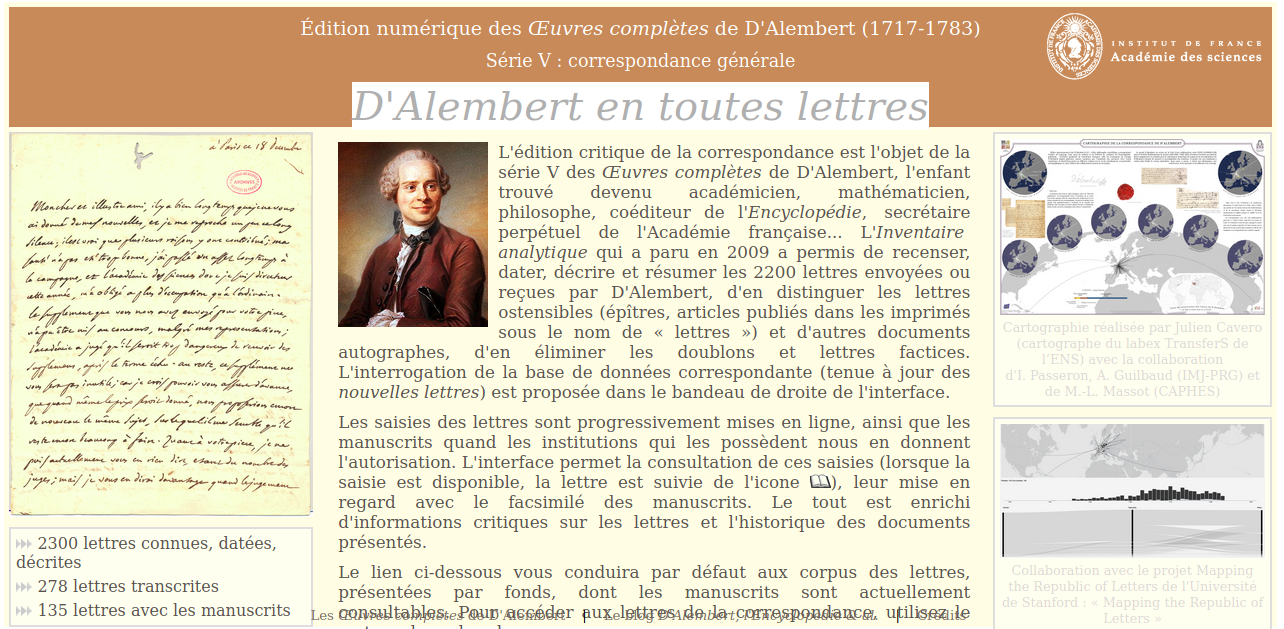
\includegraphics[width=16cm]{images/D_Alembert.png}
    \label{D_Alembert}
\end{figure}

\begin{figure}[ht]
    \centering
    \caption{ Édition numérique de la correspondance de Jean Paulhan, Labex OBVIL}
    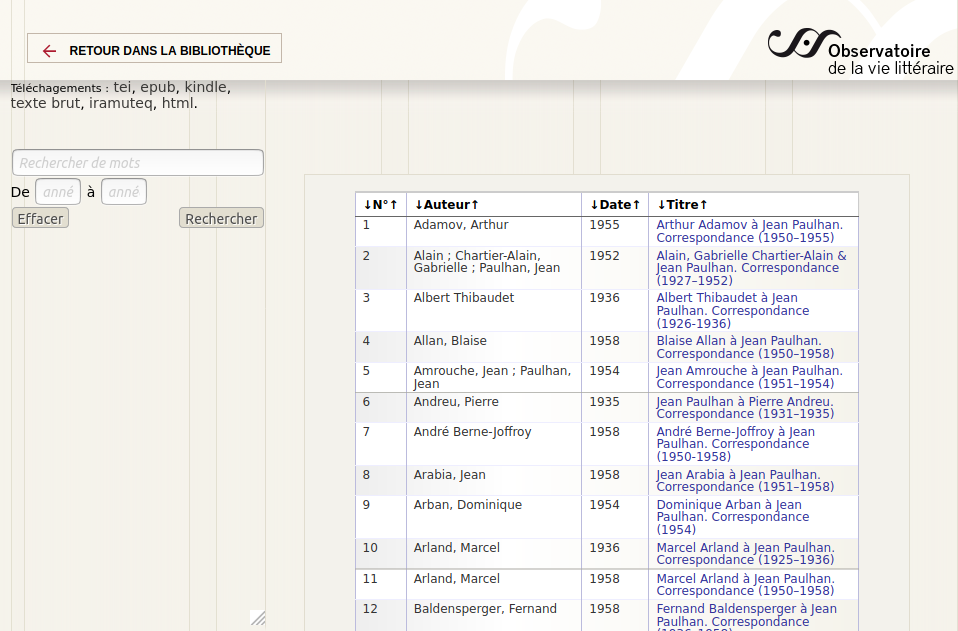
\includegraphics[width=16cm]{images/paulhan_obvil.png}
    \label{paulhan_obvil}
\end{figure}

\begin{figure}[H]
    \centering
    \caption{ Édition numérique de la correspondance de Marc Michel Rey, HUMA-NUM}
    \includegraphics[width=16cm]{images/rey.png}
    \label{rey}
\end{figure}

\begin{figure}[H]
    \centering
    \caption{Accueil de l'édition numérique de la correspondance de Gustave Flaubert, Centre Flaubert}
    \includegraphics[width=16cm]{images/accueil_flaubert.png}
    \label{accueil_flaubert}
\end{figure}

\begin{figure}[ht]
    \centering
    \caption{Lettre à Théophile Gauthier, Édition numérique de la correspondance de Gustave Flaubert, Centre Flaubert}
    \includegraphics[width=16cm]{images/flaubert_lettre.png}
    \label{flaubert_lettre}
\end{figure}

\begin{figure}[H]
    \centering
    \caption{Lettre Lionel Hauser, Édition numérique de la correspondance de Marcel Proust, Corr-Proust}
    \includegraphics[width=16cm]{images/corr-proust_lettre.png}
    \label{corr-proust_lettre}
\end{figure}

\bigskip
\section{Attentes liées à chaque type de publication}

\begin{figure}[H]
    \centering
    \caption{Grille d’évaluation des publications numériques de corpus d’auteurs}
    \includegraphics[width=16cm]{images/evaluation_publ_numiq1.png}
    \label{evaluation_publ_numiq1}
\end{figure}

\begin{figure}[H]
    \centering
    \caption{Grille d’évaluation, suite}
    \includegraphics[width=16cm]{images/evaluation_publ_numiq2.png}
    \label{evaluation_publ_numiq2}
\end{figure}

\section{Ébauche d'une arborescence}

\begin{figure}[H]
    \centering
    \caption{Ébauche de l'accueil du futur site d'édition numérique de la correspondance de Frédéric Le Play, CRHXIX}
    \includegraphics[width=16cm]{images/accueil_site_LP.png}
    \label{accueil_site_LP}
\end{figure}

\chapter{Transcription et Transkribus}

\begin{figure}[ht]
    \centering
    \includegraphics[width=14cm]{images/TRANSKRIBUS.png}
\end{figure}

\section{Les fac-similés}

On peut voir ici quelques exemples des manuscrits que nous avons au CRHXIX. On peut constater les variations d'écriture de Le Play, les différentes qualités de numérisation et les nombreux fonds différents, recélant de la correspondance de Frédéric Le Play.
Nous avons choisi de ne présenter que des lettres écrites par Le Play (excepté celle de Jules Baroche qui illustre nos propos du mémoire). Il faut cependant savoir qu'il existe bien mille lettres de correspondance passive, mais nous n'avons traité que la correspondance active donc c'est celle que nous avons choisi de mettre en valeur.


\begin{figure}[ht]
    \centering
    \caption{Lettre de Jules Baroche à Frédéric Le Play, BIF, Paris)}
    \includegraphics[width=12cm]{images/SIM-MS6062-1Baroche.png}
    \label{SIM-MS6062-1Baroche}
\end{figure}
\begin{figure}[H]
    \centering
    \caption{Lettre de Le Play à Louis de Kergorlay, 1864, Bibliothèque de l'Arsenal, Paris. Exemple typique d'un fac-similé médiocre.}
    \includegraphics[width=15cm]{images/5MS14112_p37_1p_20sept1864.jpg}
    \label{Kergorlay}
\end{figure}
\begin{figure}[H]
    \centering
    \caption{Lettre de Le Play à Ubaldino Peruzzi, 1857, BNC, FLorence. L'écriture de Le Play est plus penchée, liée et arrondie.}
    \includegraphics[width=15cm]{images/u peruzzi xxxi ins 37 (7).jpg}
    \label{peruzzi}
\end{figure}
\begin{figure}[H]
    \centering
    \caption{Lettre de Le Play à M\up{gr} Félix Dupanloup, 1873, BNF, Paris. L'écriture de Le Play est très appliquée, plus vieille également, le papier légèrement strié, la plume plus épaisse.}
    \includegraphics[width=15cm]{images/LPdupanloup2BNF9.jpg}
    \label{dupanloup}
\end{figure}
\begin{figure}[H]
    \centering
    \caption{Lettre de Le Play à Frédéric de Mercey, 1856, BNF, Paris. L'écriture de Le Play est plus hâtive, la plume plus fine.}
    \includegraphics[width=14cm]{images/mercey.JPG}
    \label{mercey}
\end{figure}
\begin{figure}[H]
    \centering
    \caption{Lettre de Le Play son fils Albert, 1865, Château de Ligoure. Le \inquote{A} de Albert s'apparente à un \inquote{a} minuscule.}
    \includegraphics[width=16cm]{images/Frédéric à Albert 001.jpg}
    \label{albertLP}
\end{figure}
\begin{figure}[H]
    \centering
    \caption{Lettre de Le Play Charles de Ribbe, 1869, Musée Arbaud, Aix-en-Provence. L'écriture est plus penchée, moins jeune.}
    \includegraphics[width=16cm]{images/ribbe.png}
    \label{ribbe}
\end{figure}

\hugeskip 

\section{Chargement des données d'entraînement}

\begin{figure}[H]
    \centering
    \caption{Problème de TR, capture d'écran de Transkribus}
    \includegraphics[width=14cm]{images/trTranskribus.png}
    \label{trTranskribus}
\end{figure}

\begin{figure}[H]
    \centering
    \caption{Résolution du problème de TR, deux sens d'écriture, capture d'écran de Transkribus}
    \includegraphics[width=14cm]{images/trCorTranskribus.png}
    \label{trCorTranskribus}
\end{figure}

\section{Schématisation du modèle d’information de Transkribus}

Schéma modèle Transkribus proposé par l'INHA\footnote{\emph{Schéma modèle Transkribus}, Site web de l'INHA, URL : \url{https://skylab.inha.fr/EditionsEnrichies/Documents/Schema-Modele-Transkribus.pdf} (visité le 18/06/2020)}.

\begin{figure}[ht]
    \centering
    \caption{Le modèle de métadonnées Transkribus, INHA}
    \includegraphics[width=11cm]{images/schema_modele_transkribus_inha1.png}
    \label{schema_modele_transkribus_inha1}
\end{figure}

\begin{figure}[ht]
    \centering
    \caption{La transcription diplomatique numérique via Transkribus, INHA}
    \includegraphics[width=16cm]{images/schema_modele_transkribus_inha2.png}
    \label{schema_modele_transkribus_inha2}
\end{figure}

\begin{figure}[ht]
    \centering
    \caption{\inquote{Cheatsheet} métadonnées Transkribus, INHA}
    \includegraphics[width=16cm]{images/schema_modele_transkribus_inha3.png}
    \label{schema_modele_transkribus_inha3}
\end{figure}

\chapter{L'encodage en XML-TEI}
\section{Les index}

\begin{figure}[H]
    \centering
    \caption{L'index de vocabulaire leplaysien, capture d'écran de l'ODD}
    \includegraphics[width=14cm]{images/indexLP.png}
    \label{indexLP}
\end{figure}

\chapter{Livrables du CRHXIX}

Pour mieux se repérer dans les livrables, il est conseillé de consulter le fichier \citecode{arborescence\_detaillee.txt} qui donne une arborescence détaillée des livrables, ou alors, pour embrasser tout dans une rapide vue d'ensemble, on consultera de préférence le fichier intitulé \citecode{arborescence.txt} qui ne fait pas le détail pièce par pièce. 

\section{\citecode{CRHXIX/rapport\_fin\_stage\_CRHXIX.pdf}}

Ces livrables ont été faits au cours de notre stage au CRHXIX qui recouvrait une période de 31,5 jours de travail.
Dans l'ensemble, les 15 premiers jours ont été consacrés à la prise en main du projet et le travail sur Transkribus, les 15 autres ont été employés à l'établissement du cahier des charges et de récits utilisateurs, dans une forme d'ébauche, permettant ainsi d'arriver au schéma XML-TEI et à l'ODD.


Pour avoir une petite vue d'ensemble du travail réalisé au cours de ce stage, il sera bon de lire le fichier \citecode{rapport\_fin\_stage\_CRHXIX.pdf} qui fait une synthèse des tâches accomplies.

\section{\citecode{CRHXIX/1-inventaires}}

\begin{itemize}
    \item Pour mieux comprendre ce qu'a été le travail de prise en main du projet, nous avons mis le fichier excel \citecode{Inventaire\_cor\_LP.xlsx} fait d'après le premier inventaire de 2005-2006 réalisé par Stéphane Baciocchi et Antoine Savoye dans \emph{La correspondance de Le Play, une source pour l'histoire des sciences sociales}, Stéphane Baciocchi in \emph{Les Études Sociales / Cairn.info}, 142-143-144 (II-2005-2006).
    \item Nous y joignons cet inventaire \citecode{Inventaire\_LP\_plain\_text\_gallica.odt} dans lequel nous avons fait mention des archives numériques en notre possession lors de ce stage.
\end{itemize}

A noter : ces documents sont encore à un stade de travail et devraient être perfectionnés. Ils ont surtout servi à la prise en main du projet à court terme.

\begin{figure}[ht]
    \centering
    \caption{Aperçu de l'inventaire de prise en mains du projet, capture d'écran, mai 2020.}
    \includegraphics[width=14cm]{images/inventaire.png}
    \label{inventaire}
\end{figure}
La couleur rouge mentionne les points obscurs et les données incertaines.

\section{\citecode{CRHXIX/2-transcriptions}}

On trouve dans ce dossier un échantillon d'une transcription réalisée par la stagiaire M. F. On peut y lire en note de bas de page les autres suggestions faites à la lecture de certains mots qui ne nous semblaient pas cohérents selon le contexte. 
Nous avons fait cela très occasionnellement, le but de notre stage étant surtout de gérer la partie technique. On voit ici l'avantage de notre formation initiale en sciences humaines qui nous permet de comprendre le fond et d'avoir une réflexion à son sujet (et donc de pouvoir corriger certaines erreurs) alors que nous sommes en train de travailler sur la partie plus technique. Cela peut être également un frein car l'important reste aussi la gestion de la partie technique.
On peut voir un exemple de ces ponctuelles corrections à la page 11 de cette transcription \citecode{LePlay\_Loyson\_MF.pdf}.

\section{\citecode{CRHXIX/3-trankribus}}

Ce dossier comprend les tutoriels que nous avons réalisés pour la prise en main de Transkribus.
Cela permettra à l'équipe du CRHXIX de continuer notre travail après notre départ, afin d'éviter le \inquote{facteur d'autobus} (en anglais \inquote{\emph{bus factor}}) provoqué par l'absence de partage d'informations et de compétences.

\begin{itemize}
    \item Les membres de l'équipe du CRHXIX pourront donc, grâce au fichier\\ \citecode{Tuto1\_préparation\_des\_donnees\_transkribus.pdf} apprendre à préparer les données en vue de l'entraînement d'un modèle expliqué dans le fichier\\ \citecode{Tuto2\_entraînement\_du\_modèle.pdf}.
    \item Le fichier \citecode{Tuto3\_application\_du\_modele.pdf} explique ensuite comment l'appliquer pour transcrire automatiquement.
Ils pourront donc, s'ils estiment que c'est pertinent, outre le fait de continuer à entraîner le modèle Le Play, en créer d'autres sur les correspondants les plus importants.
Et quoi qu'il en soit, ils pourront prendre en main Transkribus pour les simples transcriptions ce qui sera déjà un bon point pour le projet.
\item Enfin, le fichier \citecode{Tuto4\_exportation\_transkribus.pdf} explique comment exporter les données du serveur Transkribus à notre ordinateur. En effet, il est important de garder la main sur nos données.
\end{itemize}


En guise de complément à ce tutoriel, se trouve dans le dossier \citecode{export\_test} un test d'export des données de Transkribus vers l'ordinateur. Il est à noter que les fichiers ne sont pas encore nommés dans la forme qu'ils prendront, telle qu'on a pu la constater dans le dossier numérisation. 
\begin{itemize}
    \item On trouve ainsi dans le dossier \citecode{BNF9enJPG}, comprenant les lettres de Le Play à Monseigneur Félix Dupanloup, un export des fichiers transcrits en XML-TEI avec les numérisations correspondantes. 
    \item De même pour les lettres de Le Play à Charles de Ribbe \citecode{LP\_à\_Charles\_de\_Ribbe1} : on trouve toujours un fichier XML-TEI regroupant l'ensemble des lettres, ici\\ \citecode{LP\_à\_Charles\_de\_Ribbe\_tei.xml}, puis dans le dossier \citecode{page} un fichier XML-TEI par page transcrite (et non par lettre transcrite). Il est intéressant de constater ici le test qui a été fait : nous avons utilisé, notamment à la page 4, les \emph{tags} Transkribus et nous avons ensuite exporté en XML pour voir ce que cela donnerait. Or, ces tags se traduisent par des balises et attributs qui ne sont visibles que dans le fichier XML général et non par page. Par ailleurs, leur nommage est souvent invalide. Tout ceci est développé dans le mémoire.
    \item Le dossier \citecode{LP\_à\_Charles\_de\_Ribbe2} comprend l'export d'une sélection plus restreinte de lettres mais avec des \emph{tags} plus poussés. Il a été fait plus récemment. Il comprend également un export en \citecode{.txt}, ce qui permet une comparaison avec l'export .\citecode{xml}.
    \item Dans le dossier \citecode{Set\_entrainement\_le\_play}, l'export a été fait dans plusieurs formats. Pour les fichiers \citecode{.docx}, \citecode{.pdf}, \citecode{.xlsx}, cela n'a pas fonctionné. En revanche, les formats \citecode{.txt} et \citecode{.xml} ne présentent pas d'anomalie. Or, c'est ce qui nous intéresse donc l'expérience s'avère concluante.
\end{itemize}


Le dossier Transkribus comprend également un rapport réalisé sur l'apport de Transkribus au projet.
Ce rapport \citecode{Point\_Transkribus.pdf}, rédigé à la moitié de notre stage, a été transmis au CRHXIX en juin. Il a été partiellement repris dans notre mémoire avec des réflexions mises à jour selon le recul que nous avons actuellement.


\section{\citecode{CRHXIX/4-cahier\_des\_charges}}

Une partie importante de la mise en pratique du projet a été l'établissement d'un cahier des charges. C'est un bien grand mot étant donné que nous n'avons pas eu le temps de le mener à terme. 
C'est donc plutôt un rapport menant à la réalisation d'un futur cahier des charges qui sera vraiment réalisé par la suite.

En complément de cette ébauche de cahier des charges, on trouve un fichier excel nommé \citecode{users\_stories\_LP\_V3.ods} dans lequel sont écrits des récits utilisateurs ou \emph{users stories} permettant de mieux cerner les attentes des futurs visiteurs et utilisateurs de l'édition numérique et donc d'adapter notre édition à leurs besoins. 
Là encore, ces US gagneraient à être améliorés.

Nota : à chaque fois, on trouve le nommage V2 ou V3 à la fin des noms de fichiers. Cela signifie que nous avons fait plusieurs versions et que nous mettons la dernière (V1~= version 1, V2~= version 2, V3~= version 3 et ainsi de suite).

\section{\citecode{CRHXIX/5-site}}

Il a fallu penser le site de l'édition numérique.
C'est encore une ébauche de réflexion qui sera continuée par un membre de l'équipe du CRHXIX.

On trouve ici :
\begin{itemize}
    \item Dans le dossier \citecode{pages} les pages du site telles qu'elles ont été pensées pour l'édition numérique de la correspondance de Le Play.
    \item Le fichier \citecode{architecture\_site\_LP.JPG} présente l'architecture. Les numéros qui y sont inscrits renvoient aux fichiers du dossier \citecode{page}
\end{itemize}


\section{\citecode{CRHXIX/6-index}}

Une fois que l'on s'est fait une idée plus précise des attentes des utilisateurs et des besoins du site, il s'agit d'entreprendre la mise en oeuvre technique pour répondre à ces attentes.
Un des points importants est la réalisation d'index.
Il a été convenu pour les choix éditoriaux que nous ferions plusieurs index~: un index pour les noms de personnes, un pour les noms de lieux, un pour les grands événements, un pour les noms d'organisation, un pour les ouvrages cités, un pour les termes leplaysiens ou tout au moins sociologiques.
Pour ce dernier, il a été nécessaire de mener une réflexion plus importante pour savoir en amont quels termes nous indexerions. Pour cela, nous avons sélectionné certains mots qui nous paraissaient importants dans les lettres que nous avions déjà croisées, et nous avons soumis cet index au Professeur Antoine Savoye.
Le fichier nommé \citecode{Vocabulaire leplaysien - mots à ajouter.doc} contient les mots que nous lui avons soumis et qui ont été retenus. 
Il ne nous a pas paru intéressant de mettre les autres index dans les livrables.
En revanche, nous les avons mis dans leur forme provisoire, tels qu'ils seront utiles pour l'encodage TEI dans le dossier suivant.


\section{\citecode{CRHXIX/7-index\_tei}}

Ce dossier comprend les index en cours de constitution, tels qu'ils apparaîtront dans les lettres encodées en XML-TEI.
À chaque index correspond un fichier recensant les noms dans leur forme finale en XML-TEI. Cela permettra à la personne qui prendra la suite, d'une part d'avoir un modèle à suivre, d'autre part de pouvoir lister chaque nom rencontré et de se contenter de faire un copier/coller lors de l'encodage suivant.

On trouve donc ici :
\begin{itemize}
    \item l'index des noms d'événement~: \citecode{index\_evenements\_tei.pdf}
    \item l'index des termes leplaysiens et sociologiques~: \citecode{index\_leplaysien\_tei.pdf}
    \item l'index des noms de lieu~: \citecode{index\_lieux\_tei.pdf}
    \item l'index des noms d'organisation~: \citecode{index\_organisations\_tei.pdf} 
    \item l'index des noms d'ouvrages : \citecode{index\_ouvrages\_tei.pdf}
    \item l'index des noms de personnes et personnages : \citecode{index\_personnes\_tei.pdf} 
\end{itemize}

En outre, une recension des formes normalisées de correspondants à renseigner dans le \citecode{<teiHeader>} se trouve dans le fichier intitulé \citecode{index\_correspondants\_teiHeader.pdf}.

On aurait pu faire un index pour aider les transcripteurs à remplir les informations sur les origines du document, mais nous avons estimé que le fichier\citecode{ xxxx\_base.xml} (voir le point 8 sur la tei ) fait pour chacun des documents suffisait.

\section{\citecode{CRHXIX/8-tei}}

Dans ce dossier se trouvent les premiers essais d'encodage qui ont permis de réaliser ensuite l'ODD. 
\begin{itemize}
    \item le dossier \citecode{lp\_dupanloup\_xml} comprend les premiers essais d'encodage en XML-TEI.
  Ils sont nommés respectivement \citecode{lp\_dupanloup\_bnf-l1.xml} et \citecode{lp\_dupanloup\_bnf-l2.xml} (\citecode{lp} pour leplay, on indique toujours l'auteur des lettres en premier ; \citecode{dupanloup} pour le destinataire, \citecode{bnf} pour le lieu de conservation du fonds, \citecode{lxxx} pour le numéro de la lettre. Ici, les lettres 1 et 2).
  Le fichier \citecode{lp\_dupanloup\_bnf\_base.xml} comprend tous les éléments communs aux manuscrits écrits de Le Play à Dupanloup. Il sert de base à l'encodage de chacune des lettres.
    \item même principe pour le dossier \citecode{lp\_ribbe\_arbaud\_xml}
    \item le fichier \citecode{essai\_tei\_correspondance\_CRHXIXv2.xml} est un essai (très perfectible) d'encodage qui a aidé à la réflexion d'encodage en vue de l'ODD.
    \item  le fichier \citecode{Tuto\_XML-TEI\_CHRXIX.pdf} est un tutoriel qui a été réalisé pour le CRHXIX par nos soins, afin d'aider l'équipe du Centre dans les futurs encodages.
\end{itemize}



\section{\citecode{CRHXIX/9-odd}}

Les réflexions sur l'encodage en XML-TEI aboutissent à l'ODD (\emph{One Document Does it all}).
Ce dossier comprend :
\begin{itemize}
    \item l'ODD en html \citecode{ODD\_LEPLAY\_V1.html}
    \item un dossier \citecode{LP\_testODD} qui contient les test réalisés sur un fichier XML lié à l'ODD par un schéma relaxNG. 
\end{itemize}

L'ODD est perfectible. En quinze jours travaillés, nous n'avons pas eu le temps d'avoir une vue assez complète des milliers de lettres en notre possession, mais c'est déjà un bon point de départ pour l'encodage, et nous pensons qu'il ne devra pas être beaucoup modifié. Mais il devra l'être un peu, c'est inévitable.

\chapter{Livrables du Labex OBVIL}


Le stage au Labex Obvil recouvre une totalité de 20 jours travaillés.

Le fichier \citecode{rapport\_fin\_stage\_OBVIL.pdf} est le rapport qui a été écrit en fin de stage dans le but d'informer le chef de projet, Monsieur Glenn Roe, du travail accompli.

On trouvera sur Github les rapports qui ont été faits au quotidien à partir d'une certaine date, et une bonne partie des fichiers réalisés : \url{https://github.com/OBVIL/elicom/tree/master/extraction\_cor\_stage2020}. 
Néanmoins, il nous a paru plus clair d'en faire une sélection ici et de l'expliquer de la même manière que nous l'avons fait pour le CRHXIX, afin de garder une cohérence de moyens.

\section{Les fichiers XML-TEI}

Le dossier intitulé \citecode{extraction\_cor\_stage2020} rassemble l'ensemble des livrables d'Obvil.
\begin{itemize}
    \item \citecode{extraction\_cor\_stage2020/cor\_lamartine} : les fichiers en lien avec la correspondance d'Alphonse de Lamartine. Total de 97 fichiers XML-TEI extraits et corrigés.
    \item \citecode{extraction\_cor\_stage2020/cor\_lamennais} : ceux qui traitent de la correspondance de l'Abbé Félicité de Lamennais. Total de 204 fichiers. Certains sont nommés a, b, c car ils ont dû être divisés a posteriori. Nous avons corrigé 80 fichiers. Il faut encore corriger 124 fichiers, à savoir les fichiers 164 à 195, 2 à 9, 17 à 99.
    \item \citecode{extraction\_cor\_stage2020/cor\_proudhon} : ceux concernant Pierre-Joseph Proudhon. Total de 87 fichiers extraits et corrigés.
\end{itemize}



\section{Organisation des dossiers}

Les dossiers sont toujours organisés de la même manière au sein de chaque dossier \citecode{cor\_nomDuCorrespondant}, reflet de ce travail plus systématique.
Dans chacun on trouve les dossiers suivants :

\subsection{\citecode{corpus}}

Il rassemble d'une part le PDF extrait sur Gallica et dont nous nous servons pour repérer la mise en page et les passages versifiés afin de bien encoder, d'autre part l'extraction de l'OCR de ce même volume, en HTML. L'HTML a été corrigé par nos soins pour en assurer la validité.


\subsection{\citecode{\emph{script}}}

Comme son nom l'indique, il renferme le \emph{script} Python qui permet de passer de l'OCR HTML à un fichier XML par lettre. Le squelette est commun pour les auteurs, mais adapté aux variations de chacun.
Il est de qualité inégale. Le temps nous a manqué pour parfaire le premier \emph{script} réalisé (Lamartine).


\subsection{\citecode{dump}}

Il contient les extractions XML corrigées (sauf pour Lamennais où seulement une partie est corrigée, comme indiqué dans le rapport).

\subsection{\citecode{remarques}}
Sur Github, on peut voir les rapports écrits au jour le jour mais qui n'ont pas grand intérêt. 
Nous avons mis ici les fiches faites au fur et à mesure de notre travail, mais qui ont un aspect souvent de réflexion et d'ébauche, car ils ont été faits selon le cours de nos réflexions, qui sont peut-être plus avancées aujourd'hui. Certains des questionnements ont été résolus.
On trouve également des index de noms normalisés pour permettre de faire par la suite des copier/coller et avancer plus vite dans la correction des fichiers XML-TEI.

\backmatter

% bibliographie
\part*{Bibliographie}
\addcontentsline{toc}{part}{Bibliographie}
\markboth{Bibliographie}{Bibliographie}
\nocite{*}
\pagestyle{myheadings}
%\printbibliography[keyword=,title={}]

% Biblio sur la présentation des institutions
\printbibliography[keyword=OC,title={Le Labex OBVIL et le CRHXIX}]

% Biblio sur Le Play
\printbibliography[keyword=LP,title={Frédéric Le Play}]

% Biblio sur l'édition numérique de correspondance
\printbibliography[keyword=numerique,title={L'édition numérique de correspondance}]

% Biblio sur le ML
\printbibliography[keyword=ML,title={L'apprentissage machine, OCR et HTR}]

% Biblio sur transkribus
\printbibliography[keyword=transkribus,title={Transkribus}]

% Biblio sur XML-TEI et encodage
\printbibliography[keyword=TEI,title={L'encodage, XML-TEI et ODD}]

% Biblio sur le CDC, Site et SEO
\printbibliography[keyword=CDC,title={Le cahier des charges, la conception du site et le SEO}]

% Biblio numérique en général
\printbibliography[keyword=numiq,title={Les humanités numériques et le numérique en général}]

% Biblio sur packages python
\printbibliography[keyword=PC,title={\emph{Packages} Python utilisés}]

% Biblio sur logiciels et services
\printbibliography[keyword=LS,title={Logiciels, services et outils utilisés}]

% glossaire
\chapter*{Glossaire}
\addcontentsline{toc}{chapter}{Glossaire}
\markboth{Glossaire}{Glossaire}
\pagestyle{myheadings}

\begin{itemize}
    \item \textbf{Bibliothèque numérique} : Ensemble organisé de documents nativement numériques ou numérisés accessibles à distance par internet.
    \item \textbf{Format} : Manière normalisée de représenter des données ou des fichiers sous la forme d'informations binaires.
    \item \textbf{ID} : \emph{IDentifier}, abréviation anglaise de identification ou identifiant, il sert à identifier un objet précis dans un ensemble d'objets.
    \item \textbf{Interface graphique} : Par opposition à l'interface en ligne de commande, l'interface graphique désigne la manière dont est présenté un logiciel à l'écran pour l'utilisateur, permettant l'interaction entre l'humain et la machine. Une interface graphique bien conçue est ergonomique et intuitive afin que l'utilisateur la comprenne tout de suite.
    \item \textbf{Module} : En Python, un fichier pouvant contenir des fonctions, des classes et des données, et pouvant être importé dans un script.
    \item{\textbf{ODD}\textit{(One Document Does it all)}}:  Langage de définition et de maintenance dusystème TEI. Il permet la maintenance du code et de sa documentationd’une manière intégrée, à partir d’une seule source XML. Il se compose d'un schéma formel (utilisant un langage informatique tel que DTD, RELAX NG, W3C Schema, Schematron) pour contrôler l’édition et d'une documentation explicant aux utilisateurs ou développeurs les principes éditoriaux et choix de balises.
    \item \textbf{Python} : Langage de programmation informatique à usage général, multi-plateforme et \emph{open-source}.
    \item \textbf{\emph{Package}, \emph{library}} : Un ensemble de modules contenant des outils tels que des fonctions. Pour être utilisé, il doit être importé entièrement ou partiellement, par module.
    \item \textbf{Parser} : Processus d'analyse d'un élément textuel le rendant intelligible par la machine, sous la forme d'un encodage numérique.
    \item \textbf{\emph{Script}} : Un script désigne un programme, entier ou extrait, chargé d'exécuter une action prédéfinie quand un utilisateur réalise une action ou qu'une page web est en cours d'affichage sur un écran. Il s'agit d'une suite de commandes simples et souvent peu structurées qui permettent l'automatisation de certaines tâches successives dans un ordre donné. 
    \item \textbf{Standard} : Texte de référence reconnu, documenté et élaboré par un groupe de travail spécialisé, visant à harmoniser l'activité d'un secteur donné. Pour XML, les standards prennent la forme de schémas et de règles de balisage permettant de créer des documents de structures comparables au sein d'un même standard.
    \item \textbf{TEI} : \emph{Text Encoding Initiative} - Standard de description de documents textuels pour XML. Développé par le TEI Consortium.
    \item{\textbf{Transkribus}} : Plateforme de transcription automatique de textes manuscrits. Fondé sur l’intelligence artificielle, le moteur de reconnaissance de texte manuscrit (Handwritten Text Recognition ou HTR) doit être préparé avec des donnéesd’apprentissage, obtenues par la transcription d’une centaine de pages minimum, en établissant la correspondance ligne à ligne entre l’image du texte numérisé et sa transcription.
    \item{\emph{\textit{\textbf{User Story}}}} : Un récit utilisateur, ou «\textit{ user story} »  en anglais, est une description simple d’un besoin ou d’une attente exprimée par un utilisateur et utilisée dans le domaine du développement de logiciels et de la conception de nouveaux produits pour déterminer les fonctionnalités à développer.
    \item \textbf{VIAF} : \emph{Virtual International Authority File} ou Fichier d'autorité international virtuel, est un fichier d'autorité international servant à identifier les personnes ou les collectivités contenues dans d'autres fichiers d'autorité
    \item \textbf{Wiki} : Application web dont le contenu peut être édité par les visiteurs, ce qui permet la création et la modification des pages de manière collaborative. Il est généralement dédié à un projet ou à une thématique précise.
    \item \textbf{XML} : \emph{eXtensible Markup Language} -  Un langage de balisage générique permettant de décrire des informations de manière organisée et standardisée. Le XML est une recommandation du W3C [\url{https://www.w3.org/XML/}].
    \item \textbf{XSLT} : \emph{Extensible Stylesheet Language Transformations} - Un langage basé sur XML permettant de styliser ou transformer des fichiers XML ou HTML.
\end{itemize}

% table des figures
\listoffigures

% table des matières
\tableofcontents

\end{document}